\documentclass[a4paper, 12pt]{report}

%%%%%%%%%%%%
% Packages %
%%%%%%%%%%%%

\usepackage[english]{babel}
\usepackage[noheader]{packages/sleek}
\usepackage{packages/sleek-title}
\usepackage{packages/sleek-theorems}
\usepackage{packages/sleek-listings}

% Custom colors
\usepackage{color}
\definecolor{deepblue}{rgb}{0,0,0.5}
\definecolor{deepred}{rgb}{0.6,0,0}
\definecolor{deepgreen}{rgb}{0,0.5,0}

%Per scrivere codice
\usepackage{listings}

\usepackage{pythonhighlight}

% Per figure nel testo
\usepackage{wrapfig}

% Per aggiungere ``Page 1 of 100''
\usepackage{lastpage}

\usepackage{mathtools}


\lstset{
	frame = single,
	numbers=left,                   % where to put the line-numbers
	numberstyle=\footnotesize,  % the style that is used for the line-numbers
	stepnumber=1,                   % the step between two line-numbers. If it is 1, each line
	numbersep=8pt                  % how far the line-numbers are from the code  
}

%\cfoot{\thepage\ of \label{LastPage}}
\cfoot{Page \thepage \hspace{1pt} of \pageref{LastPage}}

%%%%%%%%%%%%%%
% Title-page %
%%%%%%%%%%%%%%

\logo{./resources/img/logo.png}
\institute{Ca' Foscari University}
\faculty{Faculty of Computer Science}
%\department{Department of Anything but Psychology}
\title{Cryptography}
\subtitle{Afternotes}
\author{\textit{Author}\\Francesco \textsc{Vivian}}
%\supervisor{Linus \textsc{Torvalds}}
%\context{Well, I was bored...}
\date{A.Y. 2020-2021}

%%%%%%%%%%%%%%%%
% Bibliography %
%%%%%%%%%%%%%%%%

\addbibresource{./resources/bib/references.bib}

%%%%%%%%%%
% Others %
%%%%%%%%%%

\lstdefinestyle{latex}{
    language=TeX,
    style=default,
    %%%%%
    commentstyle=\ForestGreen,
    keywordstyle=\TrueBlue,
    stringstyle=\VeronicaPurple,
    emphstyle=\TrueBlue,
    %%%%%
    emph={LaTeX, usepackage, textit, textbf, textsc}
}

\FrameTBStyle{latex}

\def\tbs{\textbackslash}

%%%%%%%%%%%%
% Document %
%%%%%%%%%%%%

\newtheorem{definition}{\textbf{Definition}}
\newtheorem{property}{\textbf{Property}}
\newtheorem{example}{\textbf{Example}}
\newtheorem{exercise}{\textbf{Exercise}}
\newtheorem{theorem}{\textbf{Theorem}}
\newtheorem{lemma}{\textbf{Lemma}}

\begin{document}
    \maketitle
    %\romantableofcontents
\chapter*{Lecture 1}
\begin{definition}
	Security: it generically refers to the possibility of "protecting" information, which is either stored in a computer system or transmitted on a network.
\end{definition}
Whatever will be shown works in both situations.\\
To decide whether a computer system is "secure", you must first decide what secure means to you, then identify the threats you care about. Some threats are: cyberterrorism, denial of service, modified databases, virus, identity theft, stolen customer data, equipment theft, espionage.

\vspace{5mm}
There are different aspects to protect through security properties:
\begin{property}
	Authenticity: an entity should be correctly identified.
\end{property}
\begin{example}
	Some examples of authenticity:
	\begin{itemize}
		\item login process for authenticating a user (User Identification)
		\item a digital signature allows for authenticating the entity originating a message (Message Authentication)
	\end{itemize}
\end{example}
\vspace{5mm}
\begin{property}
	Confidentiality (secrecy): information should only be accessed (read) by authorized entities.
	\begin{itemize}
		\item Confidential information is not disclosed to unauthorized individuals (Data confidentiality)
		\item Individuals control what information related to them may be collected and stored and by whom that information may be disclosed (Privacy)
	\end{itemize}
\end{property}
\begin{example}
	Some examples of confidentiality:
	\begin{itemize}
		\item the person that accesses a database should be authorized to access the data
		\item personal privacy, my private data should be protected while browsing the web
	\end{itemize}
\end{example}
The "access control" for confidentiality:
\begin{itemize}
	\item use the "need to know" basis for data access. How do we know who needs what data? (Approach: access control specifies who can access what). How do we know a user is the person she claims to be? We need her identity and we need to verify this identity (Approach: identification and authentication).
	\item Analogously, the "need to access/use" is the basis for access to physical assets (access to a computer room, use of a desktop)
\end{itemize}
Confidentiality is difficult to ensure and easy to assess in terms of success: it is binary in nature (Yes/No).
\vspace{5mm}
\begin{property}
	Integrity: information should only be modified by authorized entities.
	\begin{itemize}
		\item information and programs are changed only in a specified and authorized manner (Data integrity)
		\item a system performs its intended function, free from unauthorized manipulation (System integrity)
	\end{itemize}
\end{property}
\begin{example}
	We should not alter bank accounts and IoT device firmware.
\end{example}
If we don't have integrity, we also don't have confidentiality (with integrity I want only authorized users to be able to modify information, with confidentiality I want only authorized users to be able to see information, modifying includes seeing).
Integrity is more difficult to to measure than confidentiality, it is non binary (it has degrees of integrity) and it is content-dependent (it means different things in different context)
\begin{example}
	A quotation from a politician, we can preserve the quotation (data integrity) but mis-attribute (origin integrity), like \textit{Y said that} instead of \textit{X said that}. 
\end{example}
\vspace{5mm}
\begin{property}
	Availability: information should be available/usable fastly by authorized users.
\end{property}
\begin{example}
	It is important to guarantee reliability and safety. Apart from attacks, availability might be loss in case of faults (we need to use fault-tolerant techniques). We need availability in case of a remote surgery for example (good QoS).
\end{example}
We can say that an asset (a resource) is available if:
\begin{itemize}
	\item it provides a timely request response
	\item it provides fair allocation of resources (no starvation)
	\item it is fault tolerant (no total breakdown)
	\item it is easy to use in the intended way
	\item it provides controlled concurrency (concurrency control, deadlock control, ..)
\end{itemize}
\vspace{5mm}
\begin{property}
	Non-repudiation: an entity should not be able to deny an event. 
\end{property}
\begin{example}
	Having sent/received a message. This property is crucial for e-commerce, where "contracts" should not be denied by parties.
\end{example}
\vspace{5mm}
Other properties that are not addressed in detail are: fairness of contract signing, privacy, anonimity and unlinkability, accountability, ..
\subsubsection{Typical attacks}
We will now see some typical attacks. We assume that information is flowing from a source to a destination (e.g.: reading data is a flow from the data container to a user, writing is a flow from a user to the file system).\\

\begin{wrapfigure}[9]{l}{0.4\textwidth}
	%\centering
	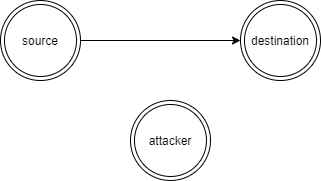
\includegraphics[width=0.37\textwidth]{images/attacks1.png}
	\caption{Expected information flow}
	\label{fig:attacks1}
\end{wrapfigure}
Malicious users might try to subvert the properties previously mentioned in many different ways. We will now give a general classification depending on how an attacker might interfere on the expected flow of information (Figure \ref{fig:attacks1}).

\begin{wrapfigure}[5]{r}{0.4\textwidth}
	%\centering
	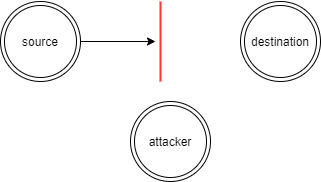
\includegraphics[width=0.37\textwidth]{images/attacks2.png}
	\caption{The attacker interrupts the flow of information}
	\label{fig:attacks2}
\end{wrapfigure}

\begin{definition}
	Interruption: the attacker stops the flow of information (Figure \ref{fig:attacks2}). The attacker interrupts a service, it breaks system integrity and availability.
\end{definition}

\vspace{5mm}
Some examples of interruption:
\begin{example}
	\leavevmode
	%Some examples of interruption:
	\begin{itemize}
		\item the destruction of a part of the hardware
		\item canceling of programs or data files
		\item the destruction of a network link
		\item a denial of service (DoS) that makes the system/network unusable 
	\end{itemize}
\end{example}

\begin{wrapfigure}[6]{l}{0.4\textwidth}
	%\centering
	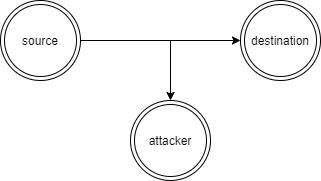
\includegraphics[width=0.37\textwidth]{images/attacks3.png}
	\caption{The attacker intercepts information}
	\label{fig:attacks3}
\end{wrapfigure}

\begin{definition}
	Eavesdropping (interception): the attacker gets unauthorized access to the information (depicted as an additional flow towards the attacker).
\end{definition}

\vspace{5mm}
Interception is an attack to confidentiality, these attacks are hard to detect.
\begin{example}
	\leavevmode
	\begin{itemize}
		\item unauthorized copies of files or programs;
		\item interception of data flowing in the network (a credit card number).
	\end{itemize}
\end{example}
\vspace{15mm}
Interception attacks are hard to detect because source and destination don't notice any change (differently from interruption, where destination don't receive the flow).


\begin{wrapfigure}[6]{l}{0.4\textwidth}
	%\centering
	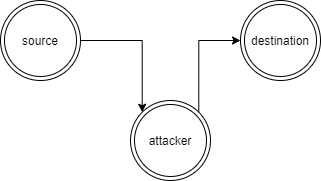
\includegraphics[width=0.37\textwidth]{images/attacks4.png}
	\caption{The attacker modifies information}
	\label{fig:attacks4}
\end{wrapfigure}

\begin{definition}
	Modification: the attacker intercepts the information and make unauthorized modification.
\end{definition}

In this case destination might notice that something is wrong.
\begin{example}
	\leavevmode
	\begin{itemize}
		\item unauthorized change of values (e.g.: of a database);
		\item unauthorized change of a program;
		\item unauthorized change of data flowing in a network;
		\item \texttt{A} redirects \texttt{S}'s bank transfer to herself (either in the browser or in the network, man in the middle).
	\end{itemize}
\end{example}

\begin{wrapfigure}[5]{r}{0.4\textwidth}
	%\centering
	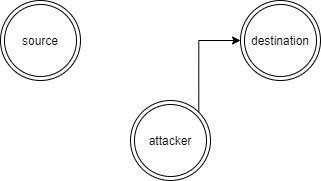
\includegraphics[width=0.37\textwidth]{images/attacks5.png}
	\caption{The attacker forges new information}
	\label{fig:attacks5}
\end{wrapfigure}

\begin{definition}
	Forging (falsification): the attacker inserts new information in the system (usually related to impersonation since the attacker lets the destination believe the information is coming from the honest source). 
\end{definition}

Forging is an attack to \textit{authenticity, accountability} and \textit{integrity}.

\begin{example}
	\leavevmode
	\begin{itemize}
		\item addition of messages in the network;
		\item addition of a record in the database.
	\end{itemize}
\end{example}

\vspace{35mm}

\begin{figure}[H]
	\centering
	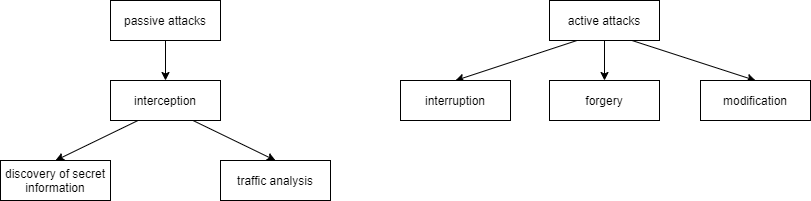
\includegraphics[scale=0.55]{images/typeofattacks.png}
	\caption{Classification of different types of attacks}
	\label{fig:typeofattacks}
\end{figure}
\newpage
\begin{example}
	Suppose a bank B is using the following simple protocol to allow a bank transfer from user Alice (A):\\
	\begin{center}
	\texttt{A $\rightarrow$ B: sign\_A("}please pay Bob 1000€\texttt{")}
	\end{center}
	\texttt{sign\_A} is some "signature" mechanism to ensure that the message really comes from Alice (thus the attacker cannot generate valid signed messages from Alice).
	
	Let's suppose Bob is the attacker, he intercepts the whole message and repeats it as many times as he want, without modifying it. This attack (called replay) consists of an interception plus forging (in this case the message is just re-sent as it is). Bob obtains many bank transfers by just re-sending message M.
\end{example}

\begin{example}
	Program modification: It is an attack to confidentiality, Bob modifies a program that is used by Alice, such a program apparently works normally, however it changes (e.g. the access rules of the users that are executing it, in this case it is called \textit{Trojan horse}). Bob waits that Alice uses the program and copies all the files of Alice in his home directory.
\end{example}

\subsubsection{Cryptography}
The term \textit{cryptography} comes from the greek and means "hidden writing". It is a way to protect the information when the environment is insecure.
For example it is used when the information is sent on a network such as internet or when the system does not support sufficient protection mechanisms.

\begin{definition}
	Encryption: a \textit{plaintext} (message) is transformed using some rules (encryption algorithm) in a ciphertext.
\end{definition}

\begin{definition}
	Decryption: the plaintext is reconstructed starting from a ciphertext.
\end{definition}

The decryption has to be simple for the receiver and unfeasible for an attacker.
The information is encrypted in the source and travels to the destination where it will be decrypted.
In order to do this there are two possible solutions:
\begin{enumerate}
	\item only the sender (Alice) and the receiver (Bob) know the encryption algorithm. If the attacker, by looking at the flow of information, is able to guess which algorithm is used, then he will be able to decrypt all the messages sent;
	\item the encryption algorithm is public and Alice and Bob share some information (the encryption key) non accessible by the attacker. If the attacker doesn't have the encryption key, it is unfeasible to decrypt the messages.
\end{enumerate}

The second solution is better because it is simpler to distribute only one key and if there is an attack it is easier to change key instead of a whole algorithm.

\begin{figure}[H]
	\centering
	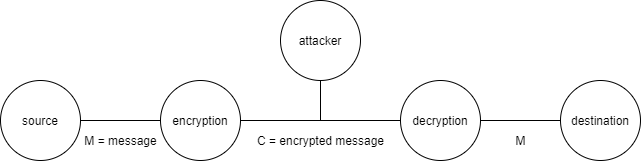
\includegraphics[scale=0.6]{images/enc1.png}
	\caption{Encryption with a shared key}
	\label{fig:enc1}
\end{figure}

We want to build a secure channel to be able to exchange the encryption key.

\begin{figure}[H]
	\centering
	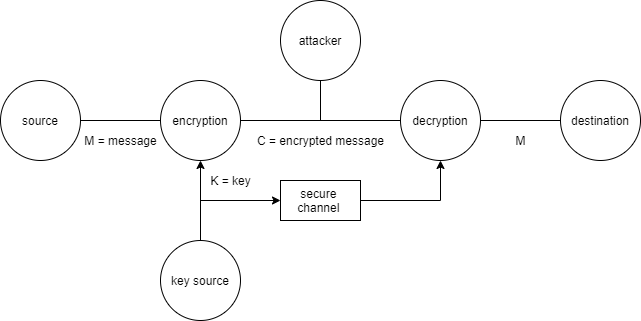
\includegraphics[scale=0.6]{images/enc2.png}
	\caption{Encryption with a shared key and the secure channel}
	\label{fig:enc2}
\end{figure}

This is called \textit{symmetric key cipher} (symmetric because source and destination use the same key).

One of the first encryption algorithms was used by Julius Caesar. In the Caesar Cipher all the letters are permuted using a certain rule (each letter is substituted by the one 3 positions ahead in the alphabet)

\begin{center}
	\texttt{A $\rightarrow$ D\\
	B $\rightarrow$ E\\
	C $\rightarrow$ F\\
	...\\
	Z $\rightarrow$ C}
\end{center}

In this case the algorithm is the Caesar Cipher and the key is 3.

\chapter*{Lecture 2}
The idea behind this course is to build step-by-step a system that is stronger and stronger until we'will arrive to systems that are used in practice.\\

Defining a cipher means to define an encryption algorithm and a decryption algorithm.\\
A \textbf{cryptosystem} (or \textbf{cipher}) can be defined as a quintuple \texttt{(P,C,K,E,D)} where:
\begin{itemize}
	\item \texttt{P} is the set of plaintexts (i.e. all the Italian words);
	\item \texttt{C} is the set of ciphertexts;
	\item \texttt{K} is the set of keys (we can have more than one key);
	\item \texttt{E:K$\times$P$\rightarrow$C} is the encryption function;
	\item \texttt{D:K$\times$C$\rightarrow$P} is the decryption function.
\end{itemize}
Let \texttt{x$\in$P, y$\in$C, k$\in$K}, we will write $E_k$(x) and $D_k$(y) to denote E(k,x) and D(k,y), the encryption and the decryption under the key k of x and y respectively.\\

We require two properties for each cipher that uses a shared key:
\begin{property}
	$D_k(E_k(x)) = x$, decrypting a ciphertext with the right key gives the original plaintext.
\end{property}
\begin{property}
	computing k or x given a ciphertext is infeasible, so complex that cannot be done in a reasonable time.
\end{property}

All the ciphers we will discuss have the first property, only "secure" ciphers have the second one (Caesar cipher doesn't). If someone, one day, will prove that P=NP, then most of the ciphers won't be secure anymore.

\begin{example}
	Referring to the Caesar cipher, we can define the encryption function as "the letter three positions ahead (of our letter x) in the alphabet" or \texttt{(x+3) mod26} and the decryption function as "the letter three position behind (of the letter to be decrypted)" or \texttt{(x-3) mod26}. Our key k=3.
\end{example}

If we find the message \texttt{"BHV BRX PDGH LW"} and we know that it is encrypted with the Caesar cipher we can easily decrypt it into \texttt{"YES YOU MADE IT"} just going back 3 positions. We can notice that we have two "B" and they correspond to the same decrypted letter "Y", in monoalphabetic ciphers this is a strong weakness.

\begin{proof}[Proof of the first property applied to the Caesar cipher]
	We have to prove that:
	\begin{align}
	x &= D_k(E_k(x)) \\
	&=((x+3) \ \textrm{mod}26 - 3) \ \textrm{mod}26 \\
	&=((x+3) - 3) \ \textrm{mod}26 \\
	&=x \ \textrm{mod}26 \\
	&=x
	\end{align}
	Since we have the modules repeated twice we can keep only the external one.
\end{proof}
To prove this property we can apply this reasoning to every cipher.\\

\begin{definition}
	Kerckhoffs' principle: a cipher should remain secure even if the algorithm becomes public.
\end{definition}

Kerckhoffs rules (1883):
\begin{itemize}
	\item The system should be, if not theoretically unbreakable, unbreakable in practice;
	\item The design of a system should not require secrecy, and compromise of the system should not inconvenience the correspondents (Kerckhoffs' principle);
	\item the key should be memorable without notes and should be easily changeable;
	\item the cryptograms should be transmittable by telegraph;
	\item the apparatus or documents should be portable and operable by a single person;
	\item the system should be easy, neither requiring knowledge of a long list of rules nor involving mental strain.
\end{itemize}


The Caesar cipher is clearly insecure (it will be proved later) since once the cipher has been broken any previous exchanged message is also broken (as the cipher works the same way), the key should be changed and it is assumed to be the only secret.

\subsubsection{Shift cipher}
We can extend the Caesar cipher to a shift cipher with a generic key k, we can choose any key in the range $0\leq k\leq 25$. For simplicity we will consider letters as numbers (\texttt{A=0, B=1, .., Z=25}), this means that $P=C=K=Z_{26}$ ($Z_{26}$ is for all the integers between 0 and 25). For the encryption and decryption function we have:
\begin{center}
	$\textrm{E}_k(x) = (x+k) \textrm{mod}26$\\
	$\textrm{D}_k(y) = (y-k) \textrm{mod}26$
\end{center}
The Caesar cipher is a subcase of a shift cipher with k=3.
In  a shift cipher is useless to have k=0 because we would end up with equals plaintexts and ciphertexts.

\begin{example}
	Considering k=10, it gives the following substitution:
	\begin{center}
		\texttt{ABCDEFGHIJKLMNOPQRSTUVWXYZ}\\
		$\downarrow$\\
		\texttt{KLMNOPQRSTUVWXYZABCDEFGHIJ}
	\end{center}
\end{example}

\begin{proof}[Proof of the first property applied to a shift cipher]
	We have to prove that:
	\setcounter{equation}{0}
	\begin{align}
		x &= D_k(E_k(x)) \\
		&=D_k((x+k) \ \textrm{mod}26) \\
		&=((x+k) \ \textrm{mod}26 - k) \ \textrm{mod}26 \\
		&=((x+k) - k) \ \textrm{mod}26 \\
		&=x \ \textrm{mod}26 \\
		&=x
	\end{align}
\end{proof}
Note that $\textrm{Z}_{26}$ is a group under the addition (but not under the multiplication).

\begin{definition}
	A \textbf{group} $\langle\textrm{G},*\rangle$ is a set G together with a (closed) binary operation * on G such that:
	\begin{itemize}
		\item the operator is associative ($(x*y)*z =x*(y*z)$ for all x,y,z in $\langle\textrm{G},*\rangle$);
		\item there is an element e$\in$G such that $a*e = e*a = a$ for all a$\in$G. Such an element is the identity element;
		\item for every a$\in$G, there is an element b$\in$G such that $a*b=e$. This b is said to be the inverse of a with respect to *. The inverse of a is sometimes denoted as $\textrm{a}^{-1}$.
	\end{itemize}
\end{definition}
\vspace{5mm}
The set $\langle\textrm{Z},+\rangle$, which is the set of integers under addition, forms a group:
\begin{itemize}
	\item addition is associative ($(x+y)+z = x+(y+z)$ for all x,y,z in $\langle\textrm{Z},+\rangle$);
	\item the identity element is 0, since $0+a = a+0 = a$ for any a$\in$Z;
	\item the inverse of any a$\in$Z is -a.
\end{itemize}
A group that is commutative with an additive operator is said to be an abelian group.

\vspace{5mm}
The set $\langle\textrm{Z},\cdot\rangle$, the set of all integers under multiplication, does not form a group. There is a multiplicative identity 1 but there is no multiplicative inverse for every element in Z.\\

From now on we will work with abelian groups.

\subsubsection{Possible attack to shift ciphers}
If I can attack a shift cipher, I can implicitly attack the Caesar cipher.
\begin{example}
	If I am an attacker, I see the message \texttt{NGPPS} and I know that it is encrypted using a shift cipher but I don't know which key k is used I can try to get it by trial and error. I start with \texttt{k=1} and if decrypting the message I obtain something nonsense, I try with k=2 and so on. with k=4 I will reach that \texttt{NGPPS=HELLO}. Is it feasible? Yes because we only have 26 possible to keys to try. This type of attack is called \textbf{Brute force}.
\end{example}

In this case the problem with our encryption algorithm is the very small number of keys. Thus the second property doesn't hold (Kerckhoffs' principle: a cipher should remain secure even if the algorithm becomes public). The weakness is that we know that each letter is moved by the same distance.

\subsubsection{Substitution cipher}
A substitution cipher is a generalization to overcome the previous limitation: instead of moving all the letters by the same distance, now we use a generic permutation of the alphabet to map the letters. For example:
\begin{center}
	\texttt{ABCDEFGHIJKLMNOPQRSTUVWXYZ}\\
	$\downarrow$\\
	\texttt{SWNAMLXCVJBUYKPDOQERIFHGZT}
\end{center}
"\texttt{HOME}" becomes "\texttt{CPYM}". In this case the key is the complete permutation, otherwise the receiver is not able to decrypt our message. As for the previous ciphers, to decrypt we just apply the inverse substitution.\\
We have P=C=$\textrm{Z}_{26}$ and K=\{p|p is a permutation of 0,..,25\} with:
\begin{itemize}
	\item $\textrm{E}_k$(x)=$\rho$(x);
	\item $\textrm{D}_k$(y)=$\rho^{-1}$(y).
\end{itemize}

Can we "Brute force" also this type of ciphers? No, we would have to try 26! keys, which is approximately $4\times10^{26}>2^{88}$. This number of keys is very heavy to brute force, even with powerful parallel computers. We have to find something different to attack substitution ciphers. How can we do it?\\

It is a monoalphabetic cipher (it maps a letter to the very same letter), this preserves the statistics of the plaintext and makes it possible to reconstruct the key by observing the statistics in the ciphertext. For example, in Italian, almost all the words end with a vowel, and the vowels (a,e,i,o,u) are easy to identify as they are much more frequent than the other letters.\\

Let us assume a cryptoanalyst knows the used cipher (e.g. a monoalphabetic substitution cipher) and the language used in plaintext (e.g Italian), but he doesn't know the plaintext and the key.

\begin{example}
	Given a ciphertext C, let us compute the frequency of letters, for example lette S appears 0 times and letter C appears 15 times. Is it possible that the cipher transforms A into S, and Z into C (A is never found and Z is found 15 times)? It is possible but very unlikely.
\end{example}

To compute the statistics for letters in Italian language it has been used a text of 14.998 letters, 1/3 from the book "Pinocchio" and 2/3 from the book "Il nome della rosa". The letters frequency are reported in the following table.
\newpage
\begin{table}[h!]
	\centering
	\begin{tabular}{||c | c | c||} 
		\hline
		\textbf{Letter} & \textbf{Absolute frequency} & \textbf{Percentage frequency} \\ 
		\hline\hline
		A & 1714 & 0.114 \\ 
		\hline
		B & 160 & 0.011 \\ 
		\hline
		C & 637 & 0.042 \\ 
		\hline
		D & 566 & 0.038 \\ 
		\hline
		E & 1658 & 0.111 \\ 
		\hline
		F & 141 & 0.009 \\ 
		\hline
		G & 272 & 0.018 \\ 
		\hline
		H & 160 & 0.011 \\ 
		\hline
		I & 1563 & 0.104 \\ 
		\hline
		L & 966 & 0.064 \\ 
		\hline
		M & 436 & 0.029 \\ 
		\hline
		N & 966 & 0.064 \\ 
		\hline
		O & 1486 & 0.099 \\ 
		\hline
		P & 421 & 0.028 \\ 
		\hline
		Q & 85 & 0.006 \\ 
		\hline
		R & 978 & 0.065 \\ 
		\hline
		S & 771 & 0.051 \\ 
		\hline
		T & 1024 & 0.068 \\ 
		\hline
		U & 528 & 0.035 \\ 
		\hline
		V & 343 & 0.023 \\ 
		\hline
		Z & 123 & 0.008 \\ 
		\hline
		\textbf{Total} & \textbf{14998} & \textbf{0.998} \\ 
		\hline
	\end{tabular}
	\label{tab:italianstats}
	\caption{Letters statistics for Italian language.}
\end{table}

The most used letter is A and the less used is Q. We can also build the graph in figure \ref{fig:itastatsgraph} to represent this statistic.
\begin{figure}[H]
	\centering
	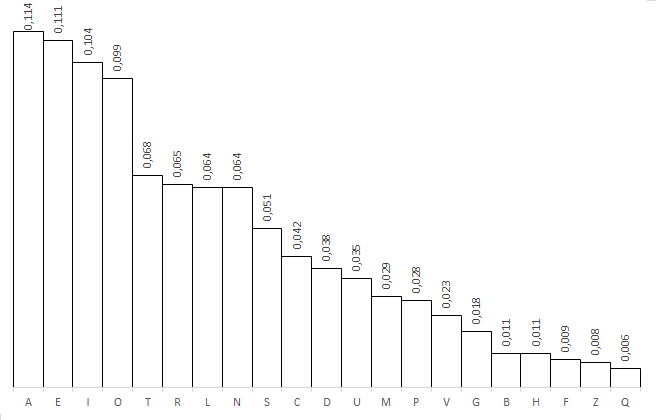
\includegraphics[scale=0.7]{images/Lec2/itastatsgraph.png}
	\caption{Percentage frequencies of letters in Italian language.}
	\label{fig:itastatsgraph}
\end{figure}
Knowing this, we can study the frequency of each letter in my ciphertext and map them using the frequency of my language.
\begin{itemize}
	\item In Italian the frequency of letters I and L increases at the beginning of the sentences (articles "il", "lo", "la"), and the frequency of "A", "E", "I", "O" at the end of the words;
	\item there are words that may appear more frequently (e.g. the word "airplane" in a  military message);
	\item there exist digraph and trigraph that are more frequent. 
\end{itemize}

How can we decrypt a message?
\begin{itemize}
	\item we order the letters of the ciphertext into decreasing frequencies;
	\item we substitute with letters in decreasing order as in the corresponding tables (depending on the language);
	\item there might be mistakes with letters that have the same frequency ("N" and "L" or "H" and "B" in Italian).
\end{itemize}

We need a long ciphertext in order to obtain reasonable frequencies.
It is possible that at the first try we obtain some nonsense words but similar to some words of complete meaning, we can then change letters to correct these words. Repeating some times this step we would end up with the correct plaintext.

We have seen that we can easily break monoalphabetic ciphers applying this method, so the second property doesn't hold. Attacks to substitution ciphers are called \textbf{Statistical attacks}

\begin{proof}[Proof of the first property applied to a substitution cipher]
	We have to prove that:
	\setcounter{equation}{0}
	\begin{align}
		x &= D_k(E_k(x)) \\
		&=D_k(\rho(x)) \\
		&=\rho^{-1}(\rho(x)) \\
		&=x\\
	\end{align}
\end{proof}

We have seen that monoalphabetic ciphers are prone to statistical attacks, since they preserve the statistical structure of the plaintext. A solution are the polyalphabetic ciphers in which the same symbol is not always mapped to the same encrypted symbol.

\subsubsection{Polyalphabetic ciphers}
An example of polyalphabetic cipher is the \textbf{Vigenére cipher} (XVI century). It works on "blocks" of \textit{m} letters with a key of length \textit{m}.
\begin{example}
	The key is \texttt{FLUTE} (m=5). The plaintext is split into blocks of length 5 and the key \texttt{FLUTE} is repeated as necessary and used to encrypt each block.
	\begin{center}
		\texttt{THISISAVERYSECRETMESSAGE}\\
		+\\
		\texttt{FLUTEFLUTEFLUTEFLUTEFLUT}\\
		=\\
		\texttt{YSCLMXLPXVDDYVVJEGXWXLAX}
	\end{center}
	\vspace{5mm}
	Each letter of the ciphertext is given by the sum of the position of the letter in the plaintext plus the position of the letter in the key.
\end{example}
This type of ciphers works better than monoalphabetic ciphers because one letter is not always mapped to the same one unless they are at a distance that is multiple of m.\\

Formally, P=C=K=Z$^m_{26}$, where Z$^m_{26}$ is Z$_{26}\times$Z$_{26}\times$..$\times$Z$_{26}$, m times.
\begin{itemize}
	\item E$_{k1,..,km}$(x$_1$,..,x$_m$) = (x$_1$+k$_1$,..,x$_m$+k$_m$) mod26;
	\item D$_{k1,..,km}$(y$_1$,..,y$_m$) = (x$_1$-k$_1$,..,x$_m$-k$_m$) mod26.
\end{itemize}

If an attacker knows m, he has to try 26$^m$ possible keys, if m is big enough, it is impossible to brute force it.

\chapter*{Lecture 3}

Vigenére cipher cause an almost "flat" distribution of letters frequency, for this reason we would make many mistakes if we try do decrypt a ciphertext in the same way as we do for monoalphabetic ciphers.

As said in the last part of the previous lesson, if we want to brute force this cipher, (assuming we know m) we would have to try 26$^m$ possible keys and that's infeasible, if we don't know m, it would we even worse. It is sufficient to choose m big enough to prevent brute force attacks, note that the number of keys grows exponentially with respect to the length.

\subsubsection{Breaking Vigenére cipher}
Even if the Vigenére cipher hides the statistic structure of the plaintext better than monoalphabetic ciphers, it still preserve most of it.

There are two famous methods to break this cipher, the first is due to Friedrick Kasiski (1863) and the second to Wolfe Friedman (1920). We will see the latter since it is more suitable to be mechanized. Both are based in \textbf{recover the length m of the key} and then \textbf{recover the key}.

The Friedman method uses statistical measures to recover the length m of the key. We consider the index of coincidence:
\setcounter{equation}{0}
\begin{equation}
	I_c(x)=\frac{\sum_{i=1}^{26} f_i(f_i-1)}{n(n-1)} \approx \sum_{i=1}^{26}p_i^2
\end{equation}
where $f_i$ is the frequency of the i-th letter in a text of length n, i.e., the number of times it occurs in such text and $p_i = f_i/n$ is the probability of the i-th letter. Intuitively, this measure gives the probability that two letters, chosen at random from the text, are the same. I compute this probability over all the letters.

\begin{example}
	The IC of \textbf{"the index of coincidence"} is given by:\\
	c(3*2) + d(2*1) + e(4*3) + f(1*0) + h(1*0) + i(3*2) + n(3*2) + o(2*1) + t(1*0) + x(1*0) = \textbf{34}\\
	divided by n(n-1)=21*20 = \textbf{420}\\
	which gives us an IC of 34/420 = \textbf{0.0809}
	
	\vspace{5mm}
	The IC of \textbf{"bmqvszfpjtcsswgwvjlio"} is given by:\\
	b(1*0) + c(1*0) + f(1*0) + g(1*0) + i(1*0) + j(2*1) + l(1*0) + m(1*0) + o(1*0) + p(1*0) + q(1*0) + s(3*2) + t(1*0) + v(2*1) + w(2*1) + z(1*0) = \textbf{12}\\
	divided by n(n-1)=21*20 = \textbf{420}\\
	which gives us an IC of 12/420 = \textbf{0.0286} 
\end{example}

Once I have the IC of my ciphertext, I have to compare it to the ICs of various languages to discover to which it corresponds.

The value of the index is maximum (value 1) for texts composed of just a single letter repeated n times.  The value of the index is minimum (value 1/26 $\approx$ 0.038) for texts composed of letters chosen with uniform probability 1/26.
 
The index of coincidence is thus a measure of how non uniformly letters are distributed in a text, each natural language has a characteristic index of coincidence, some examples:
\begin{center}
	English $\rightarrow$ 0.065\\
	Russian $\rightarrow$ 0.0529\\
	German $\rightarrow$ 0.0762\\
	Spanish $\rightarrow$ 0.0775
\end{center}

We can also use the Friedman method to find moro or polyalphabetic ciphers. We know that if we use frequencies analysis, if frequencies are flat, we have a polyalphabetic cipher, if we have peaks and valleys of frequencies, we have a monoalphabetic cipher. Considering the Friedman method, if the value of the index is minimum $\approx$ 0.038, we have a polyalphabetic cipher, if it is $\approx$ 0.065, we have a monoalphabetic cipher (same IC as English, just a permutation of letters).

With the Friedman method we can estimate m, the length of the key in a Vigenére cipher. The idea is to recover m by brute forcing, following this algorithm (in Python):

\begin{python}
	m=1
	LIMIT = 0.06 #this is to check that ICs are above 0.06 and thus close to 0.065 (assuming the text is in English)
	found = False
	while (not found):
		sub = subciphers() #takes the m subciphertexts sub[m] obtained by selecting one letter every m
		found = True
		for i in range(0,m): #compute the IC of all subtexts
			if IC(sub[i]) < LIMIT:
				#if one of the IC is not as expected try to increase the length
				found = False
				m += 1
				break
	#survived the check, all ICs are above LIMIT
	output (m)
\end{python}
It works because, once we reach the correct m, all the letters we are considering will be encrypted using the same key, "F" in the below example. So, computing the IC, we will obtain a value similar to the English IC value.
\begin{center}
	\texttt{\textcolor{red}{T}HISI\textcolor{red}{S}AVER\textcolor{red}{Y}SECR\textcolor{red}{E}TMES\textcolor{red}{S}AGE}\\
	+\\
	\texttt{\textcolor{red}{F}LUTE\textcolor{red}{F}LUTE\textcolor{red}{F}LUTE\textcolor{red}{F}LUTE\textcolor{red}{F}LUT}\\
	=\\
	\texttt{\textcolor{red}{Y}SCLM\textcolor{red}{X}LPXV\textcolor{red}{D}DYVV\textcolor{red}{J}EGXW\textcolor{red}{X}LAX}
\end{center}

In order to obtain suitable results, we need to have a long enough ciphertext, otherwise we could not be able to succeed.

Now that we have m, we need to find the key. We already said that we cannot brute force it, it would be infeasible. What should we do?
\begin{itemize}
	\item we divide the text into blocks of length m, as the length of the key (we just found it);
	\item we need to build new cryptograms with the first letter of each block, one with the second letter and so on;
	\item we analyse the new cryptograms as before and we find the shift in each position.
\end{itemize}

We are considering texts composed of letter at distance m from the first one, the second one, and so on. They have different shifts, we need to find the relative right shift.

The idea is to shift one subcipher until the mutual index of coincidence with the first subcipher becomes close to the one of the plaintext language, when this happens, we know that the applied shift is the relative shift between the two subciphers and , consequently, between the corresponding letters of the key.

The mutual index of coincidence is defined as:

\setcounter{equation}{0}
\begin{equation}
MI_c(x,x') = \frac{\sum_{i=1}^{26}f_if'_i}{nn'} = \sum_{i=1}^{26} p_ip'_i
\end{equation}
It represents the probability that two letters taken from two texts x and x' are the same.

The following algorithm selects the relative shift that maximizes the mutual index of coincidence.
\begin{python}
	key = [] #empty list
	for i in range(0,m): #for any letter of the key
		k = 0 #current relative shift
		mick = 0 #maximum index so far (we start with 0)
		for j in range(0,26): #for any possible relative shift
			#compute the mutual index of coincidence between the first subcipher
			#sub[0] and the i-th subcipher shifted by j
			mic = MIc(sub[0], shift(j,sub[i]))
			if mic > mick: #if it is the biggest so far
				k = j 		#we remember the relative shift
				mick = mic 	#.. and the maximum
		key.append(k) 		#we append to the list the shift we have found
\end{python}

We repeat this for every letter of the key and we obtain the list of relative shifts, for example, if we obtain [0,4,6,3,9], it means that the second letter of the key is equal to the first plus 4, the third is equal to the first plus 6 and so on. But what is the first letter? The final step is to try all the possible 26 letter of the key, that gives us 26 possible keys.

\subsubsection{Known-plaintext attacks}
Until now we have considered attackers that only know the ciphertext y and try to find either the plaintext x or the key k. It is often the case that an attacker can guess part of the plaintext (e.g., the "standard" header of a message), if a message is split into blocks which are encrypted under the same key, it is reasonable to assume that an attacker can deduce part of the plaintext. For example if the attacker is trying to decrypt an email, he can guess the initial par that often starts with "Dear ...".
If the attacker knows some plaintexts, this gives him the knowledge of some pairs (x,y) plaintext, ciphertext. Given this, the attacker should be able to decrypt other messages or to recover the key k (no matter which cipher is used).

The \textbf{Hill} cipher is a polyalphabetic cipher and it is a generalization of the Vigenére by introducing linear transformations of blocks of plaintext. We have P=C=Z$_m^{26}$, while K=\{K|K is an invertible mod26 matrix m$\times$m\}. The encryption and decryption are the following:
\begin{itemize}
	\item E$_K$(x$_1$,..,x$_m$) = (x$_1$,..,x$_m$)K mod26;
	\item D$_K$(y$_1$,..,y$_m$) = (y$_1$,..,y$_m$)K$^{-1}$ mod26.
\end{itemize}

\begin{example}
	Let us assume M=(x$_1$,x$_2$)=(5,9) and 
		K =$
		\begin{bmatrix}
			5 & 11\\
			8 & 3	
		\end{bmatrix}$
	(we will only consider 2$\times$2 matrices for simplicity). Thus, E$_K$(5,9) = $(5,9)\times
	\begin{bmatrix}
		5 & 11\\
		8 & 3	
	\end{bmatrix}$ mod26 = $(5\times5+9\times8,5\times11+9\times3)$ mod26 = $(25+72,55+27)$ mod26 = $(97,82)$ mod 26 = $(19,4)$
\end{example}

In order to decrypt a message, we need to compute the inverse of the matrix that is our key.
\begin{example}
	We have (y$_1$,y$_2$) = (19,4) and K=$
	\begin{bmatrix}
		5 & 11\\
		8 & 3	
	\end{bmatrix}$. To compute K$^{-1}$:\\
	K$^{-1} = $det$^{-1}$(K) $\begin{bmatrix}
		3 & -11\\
		-8 & 5	
	\end{bmatrix}$ mod26 = det$^{-1}$(K)$
	\begin{bmatrix}
		3 & 15\\
		18 & 5	
	\end{bmatrix}$ mod26.\\
\end{example}

We assume our matrix K is invertible. In the last step we changed the negative numbers to positive ones considering the mod26.

Now we can calculate det(K) = $(5\times3-11\times8)$mod26 = $(15-88)$mod26 = -73 mod26 = 5.
How do we compute det$^{-1}$(K)? To find the inverse mod26 of 5, we need to find a number in the interval [0,25] that multiplied by 5 mod26 gives 1. The number we are searching is 21, $5\times21$ mod26 = 105 mod26 = 1. Thus det$^{-1}$(K) = 21.\\
Note that it is not always the case that the multiplicative inverse modulo exists, we will discuss this more in detail later on, introducing the public key cryptography and RSA.

Now we can solve K$^{-1}$ = det$^{-1}$(K)$
\begin{bmatrix}
	3 & 15\\
	18 & 5	
\end{bmatrix}$ mod26$ = 21
\begin{bmatrix}
	3 & 15\\
	18 & 5	
\end{bmatrix}$ mod26 $=
\begin{bmatrix}
	63 & 315\\
	378 & 105	
\end{bmatrix}$ mod 26 $=
\begin{bmatrix}
	11 & 3\\
	14 & 1	
\end{bmatrix}$. Thus D$_K$(19,4)  = (19,4)$
\begin{bmatrix}
	11 & 3\\
	14 & 1	
\end{bmatrix} = (19\times11+4\times14,19\times3+4\times1)$ mod26 $=(265,61)$ mod26 $=(5,9)$.

\begin{exercise}
	Encrypt and decrypt message (2,5) using a Hill cipher with K = $
	\begin{bmatrix}
		5 & 11\\
		8 & 3	
	\end{bmatrix}$
	
	\vspace{5mm}
	\textbf{Encryption}\\
	E$_K$(2,5) = $(2,5) \times 
	\begin{bmatrix}
		5 & 11\\
		8 & 3	
	\end{bmatrix}$ mod26 $= (2\times5+5\times8,2\times11+5\times3)$ mod26 $=(10+40,22+15)$ mod26 $=(50,37)$ mod26 $=(24,11)$.
	
	\vspace{5mm}
	\textbf{Decryption}\\
	K$^{-1} = $det$^{-1}$(K) $\begin{bmatrix}
		3 & -11\\
		-8 & 5	
	\end{bmatrix}$ mod26 = det$^{-1}$(K)$
	\begin{bmatrix}
		3 & 15\\
		18 & 5	
	\end{bmatrix}$ mod26.\\
	det(K) = $(5\times3-11\times8)$mod26 = $(15-88)$mod26 = -73 mod26 = 5.\\
	det$^{-1}$(K) = 21, $5\times21$ mod26 = 105 mod26 = 1.\\
	K$^{-1}$ = det$^{-1}$(K)$
	\begin{bmatrix}
	3 & 15\\
	18 & 5	
	\end{bmatrix}$ mod26$ = 21
	\begin{bmatrix}
	3 & 15\\
	18 & 5	
	\end{bmatrix}$ mod26 $=
	\begin{bmatrix}
	63 & 315\\
	378 & 105	
	\end{bmatrix}$ mod 26 $=
	\begin{bmatrix}
	11 & 3\\
	14 & 1	
	\end{bmatrix}$.\\
	D$_K$(24,11)  = (24,11)$
	\begin{bmatrix}
	11 & 3\\
	14 & 1	
	\end{bmatrix} = (24\times11+11\times14,24\times3+11\times1)$ mod26 $=(418,83)$ mod26 $=(2,5)$.
\end{exercise}

\chapter*{Lecture 4}

\begin{figure}[H]
	\centering
	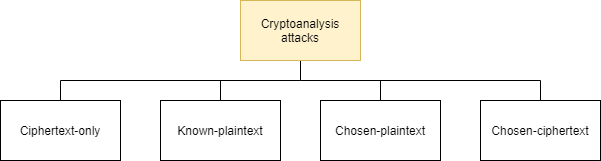
\includegraphics[scale=0.7]{images/Lec4/typesofattacks.png}
	\caption{Types of Cryptonalysis attacks.}
	\label{fig:typesofattacks}
\end{figure}

Up to now we have seen \textbf{ciphertext-only} attacks and \textbf{known-plaintext} attacks (in the last part of the previous lecture).\\
In a ciphertext-only attack, the attacker is assumed to have access only to a set of ciphertexts (e.g., monoalphabetic ciphers, polyalphabetic ciphers), the limit is that it is easy to find the correspondence between letters in the plaintext and in the ciphertext.\\
In a known-plaintext attack, the attacker knows some pairs (x',y'), (x'',y''), .. of plaintexts/ciphertexts (e.g., Hill ciphers), the limit in this case is that it is a linear transformation of plaintext block into a cipher block.

A chosen-plaintext attack (CPA) is an attack model for cryptoanalysis which presumes that the attacker can ask and obtain the ciphertexts for given plaintexts.\\
A chosen-ciphertext attack (CCA) is an attack model for cryptoanalysis where the cryptoanalyst can gather information by obtaining the decryption of chosen ciphertexts.

\begin{exercise}
	Encrypt and decrypt message (1,3) using a Hill cipher with K = $
	\begin{bmatrix}
	1 & 2\\
	4 & 3	
	\end{bmatrix}$
	
	\vspace{5mm}
	\textbf{Encryption}\\
	E$_K$(1,3) = $(1,3) \times 
	\begin{bmatrix}
	1 & 2\\
	4 & 3	
	\end{bmatrix}$ mod26 $= (1\times1+3\times4,1\times2+3\times3)$ mod26 $=(1+12,2+9)$ mod26 $=(13,11)$ mod26 $=(13,11)$.
	
	\vspace{5mm}
	\textbf{Decryption}\\
	K$^{-1} = $det$^{-1}$(K) $\begin{bmatrix}
	3 & -2\\
	-4 & 1	
	\end{bmatrix}$ mod26 = det$^{-1}$(K)$
	\begin{bmatrix}
	3 & 24\\
	22 & 1	
	\end{bmatrix}$ mod26.\\
	det(K) = $(1\times3-2\times4)$mod26 = $(3-8)$mod26 = -5 mod26 = 21.\\
	det$^{-1}$(K) = 5, $21\times5$ mod26 = 105 mod26 = 1.\\
	K$^{-1}$ = det$^{-1}$(K)$
	\begin{bmatrix}
	3 & 24\\
	22 & 1	
	\end{bmatrix}$ mod26$ = 5
	\begin{bmatrix}
	3 & 24\\
	22 & 1	
	\end{bmatrix}$ mod26 $=
	\begin{bmatrix}
	15 & 120\\
	110 & 5	
	\end{bmatrix}$ mod 26 $=
	\begin{bmatrix}
	15 & 16\\
	6 & 5	
	\end{bmatrix}$.\\
	D$_K$(13,11)  = (13,11)$
	\begin{bmatrix}
	15 & 16\\
	6 & 5	
	\end{bmatrix} = (13\times15+11\times6,13\times16+11\times5)$ mod26 $=(261,263)$ mod26 $=(1,3)$.
\end{exercise}

\subsubsection{Attack to the Hill cipher}
If I am an attacker and I have a specific number of pairs (plaintext, ciphertext), I can attack the Hill cipher. With a m$\times$m matrix, I need m pairs, if I have a 2$\times$2 matrix, I will need 2 pairs (plaintext, ciphertext) to be able to extract the key. Once I have the key, I can decrypt all the messages that will be sent later on.

We know that:
\begin{center}
	($y_1^1$, ..., $y_m^1$) = ($x_1^1$, ..., $x_m^1$)K mod26\\
	...\\
	($y_1^m$, ..., $y_m^m$) = ($x_1^m$, ..., $x_m^m$)K mod26\\
\end{center}
which can be written as Y = XK mod26 with:
\begin{center}
	X = $\begin{bmatrix}
		x_1^1 & .. & x_m^1\\
		.. & .. & ..\\
		x_1^m & .. & x_m^m	
	\end{bmatrix}$ and Y = $
	\begin{bmatrix}
		y_1^1 & .. & y_m^1\\
		.. & .. & ..\\
		y_1^m & .. & y_m^m	
	\end{bmatrix}$
\end{center}

If X$^{-1}$ exists, we can write X$^{-1}$Y mod26 = X$^{-1}$XK mod26 and then K = X$^{-1}$Y mod26.

\begin{example}
	Let's define:
	\begin{center}
		x$_1$=(5,9) $\rightarrow$ y$_1$=(19,4)\\
		x$_2$=(2,5) $\rightarrow$ y$_2$=(24,11)
	\end{center}
	We can write (19,4) = (5,9)K mod26 and (24,11) = (2,5)K mod26.\\
	We can construct X and Y matrices as follows:
	\begin{center}
		X = $\begin{bmatrix}
		5 & 9\\
		2 & 5	
		\end{bmatrix}$ and Y = $
		\begin{bmatrix}
		19 & 4\\
		24 & 11	
		\end{bmatrix}$.
	\end{center}
	Now, if X$^{-1}$ exists, we can recover the key K. We compute X$^{-1}$ in the same way we did previously for K$^{-1}$.\\
	X$^{-1}$ = det$^{-1}$(X) $\begin{bmatrix}
		5 & -9\\
		-2 & 5	
	\end{bmatrix}$ mod26 = det$^{-1}$(X) $\begin{bmatrix}
	5 & 17\\
	24 & 5	
	\end{bmatrix}$ mod26.
	
	det(X) = ($5\times5-9\times2$) = (25-18) = 7.\\
	det$^{-1}$(X)  is a number $a$ such that 7$\times a = 1$ mod26, this number $a = 15$.
	
	Thus X$^{-1}$ = det$^{-1}$(X)$\begin{bmatrix}
		5 & 17\\
		24 & 5
	\end{bmatrix}$ mod26 = 15 $\begin{bmatrix}
		5 & 17\\
		24 & 5	
	\end{bmatrix}$ mod26 = $\begin{bmatrix}
	75 & 255\\
	360 & 75	
	\end{bmatrix}$ mod26 = $\begin{bmatrix}
		23 & 21\\
		22 & 23	
	\end{bmatrix}$.
	
	\vspace{5mm}
	Then, K = X$^{-1}$Y mod 26 = $\begin{bmatrix}
		23 & 21\\
		22 & 23	
	\end{bmatrix} \begin{bmatrix}
	19 & 4\\
	24 & 11	
	\end{bmatrix}$ mod26 = $\begin{bmatrix}
		23\times19+21\times24 & 23\times4+21\times11\\
		22\times19+23\times24 & 22\times4+23\times11	
	\end{bmatrix}$ mod26 = $\begin{bmatrix}
		941 & 323\\
		970 & 341	
	\end{bmatrix}$ mod 26 = $\begin{bmatrix}
		5 & 11\\
		8 & 3	
	\end{bmatrix}$.\\
	
	So, our key K = $\begin{bmatrix}
		5 & 11\\
		8 & 3	
	\end{bmatrix}$.
\end{example}

Modern ciphers always contain a non-linear component to prevent this kind of attacks.

If th matrix X is not invertible, if the attacker has no more pairs of (plaintext, ciphertext) he lose, otherwise he can try constructing other X matrices that maybe are invertible.

\subsubsection{Block ciphers}
\textbf{Block ciphers} are cryptosystems that "reuse" the same key to encrypt letters or blocks of the plaintext. For example shift ciphers are part of block ciphers. They are weak because if an attacker know that it is always used the same key, he could recover the key and decrypt al the messages.

\begin{figure}[H]
	\centering
	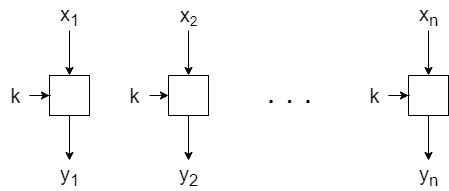
\includegraphics[scale=0.6]{images/Lec4/blockciphers.png}
	\caption{Example of block ciphers.}
	\label{fig:blockciphers}
\end{figure}
\subsubsection{Stream ciphers}
\begin{definition}
	\textbf{Stream ciphers} are cryptosystems that use a stream of key $z_1, z_2, ..., z_n$ instead of a single one.
\end{definition}
The idea is to encrypt the first letter of the plaintext with $z_1$, the second with $z_2$ and so on, it doesn't matter if we encrypt a letter or a block of text, what matters is that the key used is always different.
\begin{figure}[H]
	\centering
	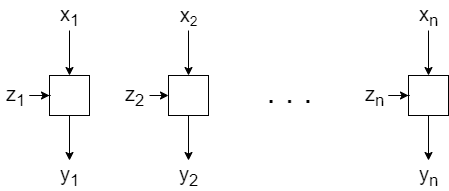
\includegraphics[scale=0.6]{images/Lec4/streamciphers.png}
	\caption{Example of stream ciphers.}
	\label{fig:streamciphers}
\end{figure}

Having a different key for each letter or block of the plaintext is of course appealing but not much practical. The stream of keys is thus usually derived starting from an initial key k, but it can also depend on previous parts of the plaintext. In general we say that
\begin{center}
	z$_i$ = f$_i$(k,x$_i$, ..., x$_{i-1}$).
\end{center}
That means that the i-th key depends on k and on the previous i-1 letters or blocks. So z$_1$ = f$_1$(k), we can compute it without knowledge of the plaintext, to compute z$_2$, instead, we need to know x$_1$ because z$_2$ = f$_2$(k,x$_1$). The values are thus computed in the following sequence: z$_1$, x$_1$, z$_2$, x$_2$, ...\\
This slow down a bit the procedure because I can't do anything in parallel.

Block ciphers are a subset of stream ciphers in which i have z$_i$=k for each i. 

A stream cipher is \textbf{periodic} if its key stream has the form:
\begin{center}
	\texttt{z$_1$, z$_2$, .., z$_d$,z$_1$, z$_2$, .., z$_d$,z$_1$, ...}
\end{center}
So if it repeats after \textbf{d} steps. This form of cipher reminds us to the \textbf{Vigenére cipher}. It can be seen as a stream cipher acting on single letters and with a periodic key stream.

\begin{exercise}
	Formalize the cipher giving (P,C,K,E,D) and defining the key stream z$_i$.
	\begin{itemize}
		\item P=C=K=Z$_{26}$;
		\item E$_{zi}$(x$_i$) = (x$_i$+z$_i$) mod26;
		\item D$_{zi}$(y$_i$) = (y$_i$-z$_i$) mod26;
		\item z$_i$ = k$_{(i \ \text{mod} \ m)}$.
	\end{itemize}
\end{exercise}

A stream cipher is \textbf{synchronous} if its key stream does not depend on the plaintexts (for example z$_i$ = f$_i$(k) for all i). So the key stream can be generated starting from k and independently on the plaintext. It is useful to improve efficiency because we do not need to obtain x$_i$ to compute z$_{i+1}$, so the key stream can be generated offline, before the actual ciphertext is received. We can consider Caesar cipher Hill cipher and also Vigenére cipher part of synchronous ciphers.

\subsubsection{Asynchronous stream ciphers}
In general asynchronous stream ciphers generate keys that depends either from k and from the previous plaintexts:
\begin{center}
	z$_i$ = f$_i$(k, x$_1$, ..., x${i-1}$)
\end{center}
This means that, if we are decrypting, we need to decrypt and, at the same time, compute the keys stream as a key can depend on previous plaintexts. An example is the \textbf{Autokey cipher}. We define it in the same way of a shift cipher, so P=C=K=Z$_{26}$ and
\begin{itemize}
	\item E$_{zi}$(x$_i$) = (x$_i$ + z$_i$) mod26;
	\item D$_{zi}$(y$_i$) = (y$_i$ - z$_i$) mod26.
\end{itemize}
We define the key stream as:
\[ z_i = \begin{cases*}
k & if  i=0  \\
x_{i-1} & if i$\ge$2
\end{cases*} \]%

The first key is the initial key k and the next keys are the same as the previous plaintext.

\begin{figure}[H]
	\centering
	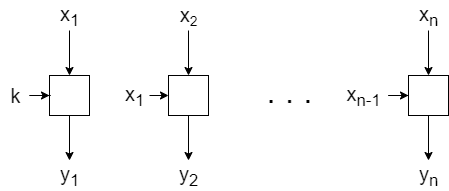
\includegraphics[scale=0.6]{images/Lec4/encautokey.png}
	\caption{Encryption in an autokey cipher.}
	\label{fig:encautokey}
\end{figure}

\begin{exercise}
	Let's assume the plaintext is the word "networksecurity", what is the encryption using k=5?\\
	First of all we need to substitute our word with the corresponding position in the alphabet and it is: "13 4 19 22 14 17 10 18 4 2 20 17 8 19 24". We will encrypt our string as follows:\\
	
	E(13) = (13+5) mod26 = 18\\
	E(4) = (4+13) mod26 = 17\\
	...\\
	E(24) = (24+19) mod26 = 17\\
	
	At this point we just need to transform back our numbers into letters and we obtain the ciphertext.
\end{exercise}

\begin{exercise}
	Try to extract the plaintext from this word encoded using Autokey. We do not know the key k.
	\begin{center}
		\texttt{FTPNIH}
	\end{center}

	Since we do not know the key k, we have to try all the 26 possible k to see which decryption produces a meaningful word.
	
	\begin{itemize}
		\item k=0 will produce \texttt{FOBMWL}, nonsense;
		\item k=1 will produce \texttt{EPANVM}, nonsense;
		\item k=2 will produce \texttt{DQZOUN}, nonsense;
		\item k=3 will produce \texttt{CRYPTO}, it has sense!
	\end{itemize}
\end{exercise}

\begin{exercise}
	Suppose that we know that \texttt{FRIDAY} has been encrypted as \texttt{PQCFKU} using the Hill cipher, What is K? Assume K is a 2$\times$2 matrix.
	
	We can consider the pairs:\\
	\texttt{(F,R) $\rightarrow$ (P,Q) = (5,17) $\rightarrow$ (15,16)}\\
	\texttt{(I,D) $\rightarrow$ (C,F) = (8,3) $\rightarrow$ (2,5)}\\
	\texttt{(A,Y) $\rightarrow$ (K,U) = (0,24) $\rightarrow$ (10,20)}\\
	
	We can construct X and Y matrices as follows:
	\begin{center}
		X = $\begin{bmatrix}
		5 & 17\\
		8 & 3	
		\end{bmatrix}$ and Y = $
		\begin{bmatrix}
		15 & 16\\
		2 & 5	
		\end{bmatrix}$.
	\end{center}
	Now, if X$^{-1}$ exists, we can recover the key K. We compute X$^{-1}$ in the same way we did previously for K$^{-1}$.\\
	X$^{-1}$ = det$^{-1}$(X) $\begin{bmatrix}
	3 & -17\\
	-8 & 5	
	\end{bmatrix}$ mod26 = det$^{-1}$(X) $\begin{bmatrix}
	3 & 9\\
	18 & 5	
	\end{bmatrix}$ mod26.
	
	det(X) = ($5\times3-17\times8$) = (15-136) = -121 mod26 = -17 mod26 = 9.\\
	det$^{-1}$(X)  is a number $a$ such that 9$\times a = 1$ mod26, this number is $a=3$.\\
	
	Thus X$^{-1}$ = det$^{-1}$(X)$\begin{bmatrix}
	3 & 9\\
	18 & 5
	\end{bmatrix}$ mod26 = 3 $\begin{bmatrix}
	3 & 9\\
	18 & 5	
	\end{bmatrix}$ mod26 = $\begin{bmatrix}
	9 & 27\\
	54 & 15	
	\end{bmatrix}$ mod26 = $\begin{bmatrix}
	9 & 1\\
	2 & 15	
	\end{bmatrix}$.
	
	\vspace{5mm}
	Then, K = X$^{-1}$Y mod 26 = $\begin{bmatrix}
	9 & 1\\
	2 & 15	
	\end{bmatrix} \begin{bmatrix}
	15 & 16\\
	2 & 5	
	\end{bmatrix}$ mod26 = $\begin{bmatrix}
	9\times15+1\times2 & 9\times16+1\times5\\
	2\times15+15\times2 & 2\times16+15\times5	
	\end{bmatrix}$ mod26 = $\begin{bmatrix}
	137 & 149 \\
	60 & 107	
	\end{bmatrix}$ mod 26 = $\begin{bmatrix}
	7 & 19\\
	8 & 3	
	\end{bmatrix}$.\\
	
	So, our key K = $\begin{bmatrix}
	7 & 19\\
	8 & 3	
	\end{bmatrix}$.
\end{exercise}

\chapter*{Lecture 5}

\begin{definition}
	A \textbf{perfect cipher} is a cipher that can never be broken, even after an unlimited time.
\end{definition}
But do perfect ciphers exist? Yes, but they are only theoretically (they can be implemented), in practice they are unpractical.

The theory behind perfect ciphers has been developed by \textbf{Claude Shannon}. It assumes an only-ciphertext model of the attacker, this means that the attacker only knows the ciphertext y and tries to find the plaintext x or the key k.

We can provide another definition for perfect ciphers:
\begin{definition}
	A cipher system is said to offer \textbf{perfect secrecy} if, on seeing the ciphertext, the interceptor gets no extra information about the plaintext than he had before the ciphertext was observed. In a cipher system with perfect secrecy, the interceptor is forced to guess the plaintext.
\end{definition}

To formalize them we need to introduce a bit of probability:
\begin{itemize}
	\item p$_p$(x) is the probability of plaintext x to occur;
	\item p$_K$(k) is the probability of certain key k to be used as encryption key.
\end{itemize}
Given a plaintext and a key there exists a unique corresponding ciphertext.

The two probability distributions p$_p$(x) and p$_K$(k) induce a probability distribution on the ciphertexts.
\setcounter{equation}{0}
\begin{equation}
	p_c(y) = \sum_{k \in K, \exists x |E_k(x)=y}^{} p_K(k)\times p_p(D_k(y))
\end{equation}

This means that, given a ciphertext y, we look for all the keys that can give such a ciphertext from some plaintext x. Then we sum the probability of all such keys times the probability of the corresponding plaintext.
\begin{example}
	Let's consider the following toy-cipher with P={a,b}, K={k$_1$,k$_2$}, C{1,2,3}. The encryption is defined in the following table:

	\begin{table}[h!]
		\centering
		\begin{tabular}{|c | c c|} 
			\hline
			\textbf{E} & \textbf{a} & \textbf{b} \\ 
			\hline
			\textbf{k$_1$} & 1 & 2 \\ 
			\textbf{k$_2$} & 2 & 3 \\ 
			\hline
		\end{tabular}
		\label{tab:exmpPerfciph}
	\end{table}

	Let p$_p$(a)=3/4, p$_p$(b)=1/4, p$_K$(k$_1$)=p$_K$(k$_2$)=1/2.
	
	Now we want to compute p$_C$(1), p$_C$(2), p$_C$(3).
	
	p$_C$(1) = p$_p$(a) $\times$ p$_{K}$(k$_1$) = 3/4 $\times$ 1/2 = 3/8\\
	p$_C$(2) = p$_p$(a) $\times$ p$_{K}$(k$_2$) + p$_p$(b) $\times$ p$_{K}$(k$_1$) = 3/4 $\times$ 1/2 + 1/4 $\times$ 1/2 = 3/8 + 1/8 = 1/2\\ 
	p$_C$(3) = p$_p$(b) $\times$ p$_{K}$(k$_2$) = 1/4 $\times$ 1/2 = 1/8\\
\end{example}

\begin{definition}
	The \textbf{conditional probability of a ciphertext} y with respect to a plaintext x, computes how likely is a certain y once we fix x.
	\setcounter{equation}{0}
	\begin{equation}
		p_c(y|x) = \sum_{k\in K, E_K(x)=y}^{} p_K(x)
	\end{equation}
	More simply is just the sum of the probability of all keys giving y from x.
\end{definition}

\begin{example}
	The conditional probability of ciphertext 1 with respect to the two plaintexts a and b is:
	
	\setcounter{equation}{0}
	\begin{align}
		p_c(1|a) &= \sum_{k\in K, E_K(x)=y}^{} p_K(x) = p_K(k_1) = 1/2 \\
		p_c(1|b) &= \sum_{k\in K, E_K(x)=y}^{} p_K(x) = 0		
	\end{align}
	We can notice that 1 can never be obtained from b. Furthermore we can see that if an attacker sees a 1, he can deduce that it is an a, this means that this is not a perfect cipher.
\end{example}

The conditional probability of a plaintext with respect to a ciphertext is related to the security of the cipher. It is a measure of how likely is a plaintext once a ciphertext is observed (which is what the attacker is usually interested to know).

With Pr(y)>0, we can define the \textbf{Bayes' Theorem} as:
\setcounter{equation}{0}
\begin{equation}
	Pr(x|y) = \frac{Pr(x) \times Pr(y|x)}{Pr(y)}
\end{equation}

We can apply this theorem to our case to get the conditional probability of a plaintext x with respect to a ciphertext y:
\setcounter{equation}{0}
\begin{equation}
	p_p(x|y) = \frac{p_p(x) \times p_c(y|x)}{p_c(y)}
\end{equation}

\begin{example}
	At this point we can compute p$_p$(a|1) and p$_p$(b|1) as follows:
	\setcounter{equation}{0}
	\begin{align}
	p_p(a|1) &= \frac{p_p(a) \times p_c(1|a)}{p_c(1)} = \frac{3/4 \times 1/2}{3/8} = 1\\
	p_p(b|1) &= \frac{p_p(b) \times p_c(1|b)}{p_c(1)} = \frac{1/4 \times 0}{3/8} = 0
	\end{align}
\end{example}
Thus, when observing a 1 as a result of a conditional probability of a plaintext x with respect to a ciphertext y, we are sure it is plaintext x, and this means that the cipher is completely insecure.

\begin{exercise}
	What will be the probabilities of plaintexts a and b with respect to ciphertext 3?
	
	First of all we need to find the conditional probabilities of ciphertext 3 with respect to the plaintexts a and b:
	
	\setcounter{equation}{0}
	\begin{align}
		p_c(3|a) &= \sum_{k\in K, E_K(x)=y}^{} p_K(x) = 0 \\
		p_c(3|b) &= \sum_{k\in K, E_K(x)=y}^{} p_K(x) = p_K(k_2) = 1/2		
	\end{align}
	
	We can now compute the conditional probabilities of plaintexts a and b with respect to the ciphertext 3:
	
	\setcounter{equation}{0}
	\begin{align}
		p_p(a|3) &= \frac{p_p(a) \times p_c(3|a)}{p_c(3)} = \frac{3/4 \times 0}{1/8} = 0\\
		p_p(b|3) &= \frac{p_p(b) \times p_c(3|b)}{p_c(3)} = \frac{1/4 \times 1/2}{1/8} =  1
	\end{align}
\end{exercise}

\begin{exercise}
	What if we compute the probabilities of a and b when observing 2?
	
	First of all we need to find the conditional probabilities of ciphertext 2 with respect to the plaintexts a and b:
	
	\setcounter{equation}{0}
	\begin{align}
	p_c(2|a) &= \sum_{k\in K, E_K(x)=y}^{} p_K(x) = p_K(k_1) = 1/2 \\
	p_c(2|b) &= \sum_{k\in K, E_K(x)=y}^{} p_K(x) = p_K(k_2) = 1/2		
	\end{align}
	
	We can now compute the conditional probabilities of plaintexts a and b with respect to the ciphertext 2:
	
	\setcounter{equation}{0}
	\begin{align}
	p_p(a|2) &= \frac{p_p(a) \times p_c(2|a)}{p_c(2)} = \frac{3/4 \times 1/2}{1/2} = 3/4\\
	p_p(b|2) &= \frac{p_p(b) \times p_c(2|b)}{p_c(2)} = \frac{1/4 \times 1/2}{1/2} =  1/4
	\end{align}
\end{exercise}

At this point we can provide an extra definition for perfect ciphers:
\begin{definition}\label{defperfcipher}
	A cipher is perfect iff p$_p$(x|y)=p$_p$(x) for all x in P and for all y in C.
\end{definition}

Intuitively, a cipher is perfect if observing a ciphertext y gives no information about any of the possible plaintexts x.

The cipher in the example is far from being perfect, but it satisfies the above definition for ciphertext 2.

A cipher is perfect if there is some key that maps any message to any ciphertext with equal probability.

\chapter*{Lecture 6}
To prove that a cipher is not perfect, we just need to find a x in P and a y in C that does not satisfy definition \ref{defperfcipher}

\begin{exercise}
	Prove that the shift cipher with p$_K$(k) = 1/|K| = 1/26 (i.e., with keys picked at random for each letter of the plaintext), is a perfect cipher. If we change key at any time we encrypt a letter, the shift cipher becomes perfect (unbreakable).
	
	We can define the cipher as follows:
	\begin{itemize}
		\item P=C=K=Z$_{26}$;
		\item E$_k$(x) = (x+k) mod26;
		\item D$_k$(y) = (y-k) mod26;
		\item k changes at each encryption.
	\end{itemize}
	We want to prove that definition \ref{defperfcipher} holds for this cipher.
	
	We compute the probability of a generic ciphertext y as:
	\setcounter{equation}{0}
	\begin{align}
	p_C(y) &= \sum_{k\in K, \exists x.E_k(x)=y}^{}p_K(k)\times p_p(D_k(y))\\
	&= \frac{1}{26} \sum_{k\in K, \exists x.E_k(x)=y}^{} p_p(D_k(y))\\
	&= \frac{1}{26}\sum_{k\in K}^{}p_p((y-k) mod26)\\
	&= \frac{1}{26}\sum_{x \in P}^{} p_p(x) = \frac{1}{26}
	\end{align}
	
	Note that for each key k, we always have the plaintext (y-k) mod26 that gives y when encrypted under k, and that for all possible keys gives all possible plaintexts x and sums to 1.
	
	\setcounter{equation}{0}
	\begin{align}
	p_c(y|x) &= \sum_{k\in K, E_k(x)=y}^{}p_K(k)\\
	&= p_K((y-x) mod26) =\frac{1}{26}
	\end{align}
	We get that k = (y-x) mod26 from the decryption formula, given x and y, there exists a unique key k that encrypts x as y and it is (y-x)mod26.
	
	Finally we can say that:
	\setcounter{equation}{0}
	\begin{align}
	p_p(x|y) &= \frac{p_p(x)\times p_c(y|x)}{p_c(y)}\\
	&= \frac{p_p(x)\times \frac{1}{26}}{\frac{1}{26}} = p_p(x)
	\end{align}
	We have demonstrated that $p_p(y|x) = p_p(x)$ for all x in P and for all y in C, thus the cipher is perfect.
\end{exercise}

\begin{theorem}\label{theoKP}
	Let $p_c(y)>0$ for all y. A cipher is perfect only if |K|$\ge$|P|.
\end{theorem}

This means that a necessary condition for a cipher to be perfect is that the number of keys is at least the same as the number of plaintexts.
\begin{proof}
	For Bayes' theorem:
		\[p_p(x|y) = \frac{p_p(x)\times p_c(y|x)}{p_c(y)}\]
	Thus, given $p_p(x|y) = p_p(x)$ (the cipher is perfect), we have $p_c(y|x) = p_c(y)$ (these two quantities erase) for all x in P and for all y in C.
	
	As an assumption $p_c(y)>0$.\\
	If we fix x, we obtain that for each y, $p_c(y|x) = p_c(y)>0$. This means that there exists at least one key k such that E$_k$(x)=y (otherwise $p_c(y|x)=0$).
	
	All such keys are different since E$_k$ is a function and we have fixed x, and x cannot be mapped to two different ciphertexts by the same key. Thus, we have at least one key for each ciphertext (|K|$\ge$|C|).
	
	Since, for any cipher (not necessarily perfect), E$_k$ injects the set of plaintexts into the set of ciphertext, we also have |C|$\ge$|P|, thus |K|$\ge$|C|$\ge$|P|, i.e.,
	\begin{center}
		\textbf{|K|$\ge$|P|}
	\end{center}
\end{proof}

\begin{exercise}
	Prove that the ciphertext defined as E$_k$(x$_1$,...,x$_d$)=(x$_1$+k,...,x$_d$+k)mod26 is not perfect.
	
	We can prove this in two ways:
	\begin{enumerate}
		\item using the theorem \ref{theoKP}, proving that |K|<|P|.\\
		Our set K=\{0, 1, 2, .., 25\}, so |K|=26, we need to find |P|. Since x=\{x$_1$,..,x$_d$\} and each x$_i$ can assume 26 values, we have that |P|=26$^d$. Thus 26<26$^d$, so |K|<|P| (with d$\ge$2). 
		\item using definition \ref{defperfcipher}. Let's assume x=\{x$_1$,..,x$_d$\} is an English word and let's also assume d=5. We are looking for an English word of length 5, for example \textit{GOOFY}. Since it is a real word, $p_p$(GOOFY)>0. We want to find a y such that $p_p$(GOOFY|y)$\ne p_p$(GOOFY)>0. For example with y=AAAAA, $p_p$(GOOFY|AAAAA)=0 and we are done. We could have used other y, such as y=ABCDE.
	\end{enumerate}
\end{exercise}

\begin{theorem}\label{theoperfcipher}
	Let |P|=|C|=|K|. A cipher is perfect iff
	\begin{enumerate}
		\item $p_K(k)=1/|K|$ for all k in K;
		\item for each x in P and y in C, there exists exactly one key k such that E$_k$(x)=y.
	\end{enumerate}
\end{theorem}
The theorem states that, for a cipher to be perfect (given that the size of P, C and K is the same), keys should be picked at random for any encryption and each plaintext is mapped into each ciphertext through a unique key.

\begin{proof}
	We will prove the $\rightarrow$ direction of the theorem.
	
	For theorem \ref{theoKP}, in a perfect cipher |K|$\ge$|C| if $p_c$(y)>0 for all y. If we fix x, we obtain that for each y $p_c$(y|x)=$p_c$(y)>0, i.e., there exists at least one key k such that E$_k$(x)=y and all of the other keys are different.
	
	Here (by assumption) |K|=|C|, meaning that all of these keys k are unique (otherwise we would have |K|>|C|). Since this holds for each x and y, we have proved condition 2, i.e., that for each x in P and y in C, there exists exactly one key k such that E$_k$(x)=y.
	
	To prove condition 1, it is enough to notice that given
	\[p_c(y|x) = \sum_{k\in K,E_k(x)=y}^{}p_K(k)\]
	$p_c$(y|x)=$p_p$(y), i.e., the probability of y given x is equal to the probability of the unique key k that encrypts x into y.
	
	Thus, $p_K$(k)=$p_c$(y|x)=$p_c$(y).\\
	If we fix y and we consider all possible plaintexts x we obtain all possible keys k and for all of them it holds $p_K$(k)=$p_c$(y). Since the number of keys is |K|, and since they all have the same probability ($p_c$(y)), and given that the sum of the probabilities of all keys must be 1 and |P|=|C|=|K|, we obtain condition 1, $p_K$(k)=1/|K|.\\
\end{proof}

We can use this theorem to prove that a cipher is (or is not) perfect.
\subsubsection{The one time pad}
This perfect cipher has been used for the telegraph and is a binary variant of Vigenére with keys picked at random.

More precisely we have P=C=K=Z$_{2^d}$ with $p_K$(k)=1/|K|=1/2$^d$ for all k in K. 2$^d$ means sequences of binary numbers of length d.

The encryption function is the following: E$_{k_1,...,k_d}$(x$_1$,...,x$_d$) = (x$_1$ xor k$_1$,...,x$_d$ xor k$_d$), where xor is a bitwise xor operation.

Is it a perfect cipher? Condition 2 of theorem \ref{theoperfcipher} is satisfied by definition. Condition 2 holds too because we are using xor operations.

\subsubsection{Lesson learned}
Shannon theory on perfect ciphers shows that they exist but require as many keys as the possible plaintexts, and keys need to be picked at random for each encryption.

Even if this makes such ciphers unpractical, the one-time-pad has been used for real transmission. The setup consisted of two identical books with thousands of "random" keys. Each key was used only once. Once the book has been used completely, new shared books were necessary.

\chapter*{Lecture 7}
\begin{exercise}
	Consider the following cipher with P=\{a,b\}, K=\{k$_1$,k$_2$,k$_3$\}, C=\{1,2,3,4\}. Encryption is defined by the following table:
		\begin{table}[H]
		\centering
		\begin{tabular}{|c | c c|} 
			\hline
			 & \textbf{a} & \textbf{b} \\ 
			\hline
			\textbf{k$_1$} & 1 & 2 \\ 
			\textbf{k$_2$} & 2 & 3 \\ 
			\textbf{k$_3$} & 3 & 4 \\ 
			\hline
		\end{tabular}
		\label{tab:exerciselec7}
	\end{table}
	We now let $p_p$(a)=1/4, $p_p$(b)=3/4, $p_K$(k$_1$)=1/2, $p_K$(k$_2$) = $p_K$(k$_3$)=1/4.\\
	Compute $p_p$(a|1), $p_p$(a|2), $p_p$(a|3), $p_p$(a|4), $p_p$(b|1), $p_p$(b|2), $p_p$(b|3), $p_p$(b|4).
	
	First of all let's compute all the $p_c$ for 1,2,3,4:
	\[p_c(1) = p_p(a)\times p_K(k_1) = 1/4\times 1/2 = 1/8\]
	\[p_c(2) = p_p(b)\times p_K(k_1)  + p_p(a)\times p_K(k_2)= 3/4\times 1/2 + 1/4\times 1/4 = 7/16\]
	\[p_c(3) = p_p(b)\times p_K(k_2)  + p_p(a)\times p_K(k_3)= 3/4\times 1/4 + 1/4\times 1/4 = 1/4\]
	\[p_c(4) = p_p(b)\times p_K(k_3) = 3/4\times 1/4 = 3/16\]
	
	Then we can compute
	\[p_c(1|a) = p_K(k_1) = 1/2\]
	\[p_c(2|a) = p_K(k_2) = 1/4\]
	\[p_c(3|a) = p_K(k_3) = 1/4\]
	\[p_c(4|a) = 0\]
	
	\[p_c(1|b) = 0\]
	\[p_c(2|b) = p_K(k_1) = 1/2\]
	\[p_c(3|b) = p_K(k_2) = 1/4\]
	\[p_c(4|b) = p_K(k_3) = 1/4\]
	
	Finally:
	\[p_p(a|1) = \frac{p_c(1|a)\times p_p(a)}{p_c(1)} = \frac{1/2\times 1/4}{1/8}= 1\]
	\[p_p(a|2) = \frac{p_c(2|a)\times p_p(a)}{p_c(2)} = \frac{1/4\times 1/4}{7/16}= 1/7\]
	\[p_p(a|3) = \frac{p_c(3|a)\times p_p(a)}{p_c(3)} = \frac{1/4\times 1/4}{1/4}= 1/4\]
	\[p_p(a|4) = \frac{p_c(4|a)\times p_p(a)}{p_c(4)} = \frac{0\times 1/4}{3/16}= 0\]
	
	\[p_p(b|1) = \frac{p_c(1|b)\times p_p(b)}{p_c(1)} = \frac{0\times 3/4}{1/8}= 0\]
	\[p_p(b|2) = \frac{p_c(2|b)\times p_p(b)}{p_c(2)} = \frac{1/2\times 3/4}{7/16}= 6/7\]
	\[p_p(b|3) = \frac{p_c(3|b)\times p_p(b)}{p_c(3)} = \frac{1/4\times 3/4}{1/4}= 3/4\]
	\[p_p(b|4) = \frac{p_c(4|b)\times p_p(b)}{p_c(4)} = \frac{1/4\times 3/4}{3/16}= 1\]
	
\end{exercise}

\subsubsection{Composition of ciphers}
A one-time-pad provides absolute security in theory, but difficult to implement in practice. Modern ciphers are based on very simple operations, such as substitution, xor, etc., that are combined in a smart way so to make the overall algorithm strong and really hard to cryptoanalyse.

Combining simple ciphers does not always improve security. Let's consider the shift cipher composed twice: we first shift by k$_1$ and then by k$_2$ modulo 26. But this is equivalent to shift by k$_1$+k$_2$ modulo 26.

\begin{example}
	Shift of 3 and then of 2:
	\begin{center}
		\texttt{ABCDEFGHIJKLMNOPQRSTUVWXYZ}\\
		\texttt{DEFGHIJKLMNOPQRSTUVWXYZABC}\\
		\texttt{FGHIJKLMNOPQRSTUVWXYZABCDE}\\
	\end{center}
	
	but this is equivalent to a shift of 5:
	\begin{center}
		\texttt{ABCDEFGHIJKLMNOPQRSTUVWXYZ}\\
		\texttt{FGHIJKLMNOPQRSTUVWXYZABCDE}\\
	\end{center}
\end{example}

\begin{definition}
	\textbf{Composition:} we consider two ciphers S$^1$=(P$^1$, C$^1$, K$_1$, E$^1$, D$^1$) and S$^2$=(P$^2$, C$^2$, K$_2$, E$^2$, D$^2$).
	
	We let P$^1$=C$^1$=P$^2$=C$^2$, that we note as P and C in the following. In this way, the output of one cipher is for sure a possible plaintext for the second cipher.
	
	We can now define the composition as S$^1\times$S$^2$=(P, C, K$_1\times$K$_2$, E, D) with:
	\begin{itemize}
		\item E$_{k_1,k_2}$(x) = E$^2_{k_2}$(E$^1_{k_1}$(x));
		\item D$_{k_1,k_2}$(y) = D$^1_{k_1}$(D$^2_{k_2}$(y));
	\end{itemize}
\end{definition}

\begin{exercise}
	Formally apply the composition of the two shift ciphers previously mentioned.
	
	Formally we have E$_k^1$(x)=E$_k^2$(x)=(x+k)mod26\\
	and\\
	E$_{(k_1,k_2)}$(x) = E$_{k_2}^2$(E$_{k_1}^1$(x)) = ((x+k$_1$) mod26+k$_2$) mod26 = (x+(k$_1$+k$_2$)mod26)mod26 = E$_{k_1+k_2mod26}^1$(x)
	
	This proves that composing the shift cipher twice is equivalent to applying it once using as a key the sum of the two keys k$_1$ and k$_2$.
\end{exercise}

\begin{exercise}
	Show that the composition of the shift cipher with the substitution cipher is still a substitution cipher with a different key. Give a constructive way to derive the new key. What happens if substitution is applied before shift? 
	
	Let's consider an example of substitution:
	\begin{center}
		\texttt{ABCDEFGHIJKLMNOPQRSTUVWXYZ}\\
		\texttt{VCFIORBMPLYUQXJHNDWSKETZAG}
	\end{center}
	If we shift of 5 (for example) and then we substitute it becomes:
		\begin{center}
		\texttt{ABCDEFGHIJKLMNOPQRSTUVWXYZ}\\
		\texttt{RBMPLYUQXJHNDWSKETZAGVCFIO}
	\end{center}
	This is nothing more then a substitution cipher with a different key. To decrypt we need to apply first the substitution and then the shift back.
	
	If we do the opposite, so first we substitute and then we shift we would have something similar to the following example:
		\begin{center}
		\texttt{ABCDEFGHIJKLMNOPQRSTUVWXYZ}\\
		\texttt{VCFIORBMPLYUQXJHNDWSKETZAG}\\
		\texttt{AHKNTWGRUQDZVCOMSIBXPJYEFL}
	\end{center}
	Once again it corresponds to a substitution cipher with a different key. Of course to decrypt we would have first to shift back and then substitute.
\end{exercise}

\begin{exercise}
	Consider the composition of a Vigenére cipher with key \texttt{ALICE} with the shift cipher with key 8. Is the resulting cipher equivalent to a known one? If so, what is the resulting key?
	
	The Vigenère cipher with key \texttt{ALICE} encryption can be represented as:
	\begin{center}
		E$_{k_1,...,k_m}$(x$_1$,...,x$_m$) = (x$_1$+0, x$_2$+11, x$_3$+8, x$_4$+2, x$_5$+4, ..) mod26
	\end{center}
	
	A shift cipher with key 8 can be represented as:
	\begin{center}
		\texttt{ABCDEFGHIJKLMNOPQRSTUVWXYZ}\\
		\texttt{IJKLMNOPQRSTUVWXYZABCDEFGH}
	\end{center}

	Then the composition is:
	E$_{k_1,k_2}$(x) = (x$_1$+0+8, x$_2$+11+8, x$_3$+8+8, x$_4$+2+8, x$_5$+4+8, ..) mod26 = (x$_1$+8, x$_2$+19, x$_3$+16, x$_4$+10, x$_5$+12, ..) mod26
	
	This is nothing more then a Vigenére cipher with key \texttt{ITQKM}
\end{exercise}

\subsubsection{Idempotent ciphers}
We have seen that the shift cipher, when repeated twice is equivalent to itself with a different key. When this happens, the cipher is said to be \textbf{idempotent}, written S$\times$S=S. In this case we know that iterating the cipher will be of no use to improve its security, even if we repeat it n times, we will still get the initial cipher, i.e., S$^n$=S.

We have mentioned that modern ciphers are based on simple operations composed together. Almost any modern cipher repeats a basic core of operations for a certain number of rounds (iteration). It is thus necessary that such core operations do not constitute an idempotent cipher.

It can be proved that if we have two idempotent ciphers that commute, i.e., such that S$^1\times$S$^2$=S$^2\times$S$^1$, then their composition is also idempotent. In this case we know that iterating their composition is useless.

\begin{proof}
	Consider one iteration of their composition
	\setcounter{equation}{0}
	\begin{align}
		&(S^1\times S^2)\times(S^1\times S^2)\\
		&=S^1\times (S^2\times S^1)\times S^2 &\text{associative property}\\
		&=S^1\times (S^1\times S^2)\times S^2 &\text{commutative property}\\
		&=(S^1\times S^1)\times (S^2\times S^2) &\text{associative property}\\
		&=S^1\times S^2 &\text{idempotence of the initial ciphers}
	\end{align}
\end{proof} 

\begin{exercise}
	Apply the above result to show that the composition of Vigenére cipher S$^1$ and the shift cipher S$^2$ is idempotent.
	
	The composition is a Vigenére cipher S$^3$ with key k$_1$+k$_2$ mod26, ..., k$_d$+k$_2$ mod26, S$^1\times$S$^2$=S$^3$.
	
	Thus (S$^1\times$S$^2$)$\times$(S$^1\times$S$^2)$ = S$^3\times$S$^3$=S$^3$ which is again a Vigenére cipher with a new key. This holds iterating many times. 
\end{exercise}

We have seen examples of how algebraic properties, such as commutativity, can help simplifying the analysis of a cipher. When developing a robust cipher, we need to avoid as much as possible that operations can be rearranged, swapped, simplified.

\section*{The Advanced Encryption Standard (AES) cipher}
AES has been selected by the National Institute of Standards and Technology (NIST) after a five-year long competition. The original name is Rijndael from the names of the two inventors, Joan Daemen and Vincent Rijmen.

As any modern cipher, AES is the composition of simple operations and contains a non-linear component to avoid known-plaintexts attacks. The composed operation give a non-idempotent cipher that is iterated for a fixed number of rounds.
\newpage
It has been selected since it provides:
\begin{itemize}
	\item high security guarantees;
	\item high performance;
	\item flexibility (different key length)
\end{itemize}
All of these features are, in fact, crucial for any modern cipher.

The Data Encryption Standard (DES) is still in use after almost 40 years, in a variant called Triple DES (3DES), which aims at improving the key length (168 bits). In fact, DES key of only 56 bits(64-8 control bits) is too short to resist brute-forcing on modern, parallel computers.

\subsubsection{Mathematical background of AES}
AES works on the Galois Field with 2$^8$ elements, noted GF(2$^8$). Intuitively it is the set of all 8-bits digits with sum and multiplication performed by interpreting the bits as (binary) coefficients of polynomials. For example 11010011 can be seen as x$^7$+x$^6$+x$^4$+x+1 and 00111010 is x$^5$+x$^4$+x$^3$+x.

The sum of x$^7$+x$^6$+x$^4$+x+1 and x$^5$+x$^4$+x$^3$+x will thus be x$^7$+x$^6$+x$^5$+x$^3$+1 since two 1's coefficient becomes 0 modulo 2=0, and the term disappears. We see that sum and subtraction are just the bit-wise XOR of the binary numbers, 11010011 XOR 00111010 = 11101001 which is x$^7$+x$^6$+x$^5$+x$^3$+1.

The product is done modulo the irreducible polynomial x$^8$+x$^4$+x$^3$+x+1, irreducible means that it cannot be written as the product of two other polynomials, it is, intuitively, the equivalent of primality.
\begin{example}
	(x$^7$+x$^6$+x$^4$+x+1)$\times$ (x$^5$+x$^4$+x$^3$+x) = x$^{12}$ + x$^{11}$ + x$^{10}$ + x$^8$ + x$^{11}$ + x$^{10}$ + x$^9$ + x$^7$ + x$^9$ + x$^8$ + x$^7$ + x$^5$ + x$^6$ + x$^5$ + x$^4$ + x$^2$ + x$^5$ + x$^4$ + x$^3$ + x = x$^{12}$ + x$^6$ + x$^5$ + x$^3$ + x$^2$ + x
	
	Now we need to divide x$^{12}$+x$^6$+x$^5$+x$^3$+x$^2$+x by the irreducible polynomial x$^8$+x$^4$+x$^3$+x+1 and find the reminder. x$^{12}$/x$^8$=x$^4$, thus (x$^8$+x$^4$+x$^3$+x+1)*x$^4$ = x$^{12}$+x$^8$+x$^7$+x$^5$+x$^4$.
	
	At this point we need to subtract this polynomial (to get the remainder), we obtain x$^8$ + x$^7$ + x$^6$ + x$^4$ + x$^3$ + x$^2$ + x and we repeat the process obtain the final remainder: x$^7$ + x$^6$ + x$^2$ + 1.  
\end{example}

\begin{exercise}
	Multiply (x$^4$+x$^3$+1)$\times$(x$^5$+1)
	
	= x$^9$+x$^4$+x$^8$+x$^3$+x$^5$+1 = x$^9$+x$^8$+x$^5$+x$^4$+x$^3$+1
	
	We divide it by the irreducible polynomial: x$^9$/x$^8$ = x, thus (x$^8$+x$^4$+x$^3$+x+1)*x = x$^{9}$+x$^5$+x$^4$+x$^2$+x.
	
	We subtract this polynomial from the result of the multiplication to obtain the reminder: x$^8$+x$^3$+x$^2$+x+1.
	
	We repeat the process and we obtain the final reminder x$^4$+x$^2$.
\end{exercise}

\chapter*{Lecture 8}
An example of optimization on numbers (on polynomial we will use XOR instead of SUM) is the following:
\begin{example}
	Let's multiplicate 11 and 1011.
	\begin{table}[H]
		\centering
		\begin{tabular}{|c|c|c|}
			\hline
			\textbf{a} & \textbf{b} & \textbf{p} \\ \hline
			11 & 1011 & 0\\
			110 & 101 & 0$\oplus$11=11\\
			1100 & 10 & 11$\oplus$110=101\\
			11000 & 1 & 101\\
			110000 & & 101$\oplus$11000 = 11101\\
			\hline
		\end{tabular}
	\end{table}
	Once we have an empty space in the \textbf{b} column, we will have the result of the multiplication in the \textbf{p} column.
\end{example}

The method seen at the end of the last lecture is, on average, quadratic with respect to the number of bits (8). Instead, the method just seen takes a number of steps equals to the length of the number in the \textbf{b} column.

\begin{python}
	def AESmult(a,b):
		p=0										#p is 0 at  the beginning
		for i in range(0,8):	#for the 8 bits of a and b do:
			if b&1 != 0:				#the least significant bit of b is set
				p = p^a						#sum a to p (xor)
			b>>=1								#shift b to the right
			hbit = (a&0x80)!=0	#true if the most significant bit of a is set
			a<<=1								#shift a to the left
			if hbit:						#if the most significant bit of a was set
				a=a^0x11b					#sum 100011011 to a xor, this always  returns a 8-bits number
		return p
\end{python}
This method works only if the resulting number smaller than x$^7$.

To test the above code it is sufficient to open a python shell (by running python from the terminal) and copy-paste the function into the shell, giving enter at the end.\\
\texttt{AESmult(0b11010011,0b00111010)} will produce 197 as result, \texttt{bin (AESmult (0b11010011, 0b00111010))} will produce 0b11000101.
\newpage
The correctness of the optimization of the product derives from invariant after each loop:
\begin{itemize}
	\item ab+p is the product of the initial a and b (all operations are done in the Galois Field);
	\item since b is 0 at the end, we have that p contains the product.
\end{itemize}

Some observations:
\begin{itemize}
	\item b is shifted to the right and a is shifted to the left, meaning that we respectively divide and multiply by x the two polynomials;
	\item if b is odd, the polynomial is not divisible by x, so we throw away the least significant bit (this is what the right shift does) and we accumulate one a in p to compensate and keep the invariant;
	\item when a becomes more than 2$^8$, we need to sum to it the modulus 100011011 (the irreducible polynomial), i.e. 0x11b, to keep it 8-bits long.
\end{itemize}

\section*{The AES cipher}
Advanced Encryption Standard (AES) is a symmetric key algorithm that uses the same key for both encryption and decryption processes, it operates on a 4$\times$4 matrix of bytes. We have that 16 bytes are 128 bits which is, in fact, the block size. Plaintext bytes b$_1$,...,b$_{16}$ are copied in the matrix by columns following this scheme:
\begin{center}$
	\begin{bmatrix}
		b_1 & b_5 & b_9 & b_{13}\\
		b_2 & b_6 & b_{10} & b_{14}\\
		b_3 & b_7 & b_{11} & b_{15}\\
		b_4 & b_8 & b_{12} & b_{16}\\
	\end{bmatrix}$
\end{center}

Cipher keys have lengths of 128, 192 and 256 bits. AES has 10 rounds for 128-bits keys, 12 rounds for 192-bits keys and 14 rounds for 256-bits keys. Rijndael was designed to handle additional block sizes and key lengths, however they are not adopted in the AES standard.

A round is composed of different operations, all of which are invertible:
\begin{itemize}
	\item bitwise xor;
	\item fixed non-linear substitution;
	\item shifting of matrix rows;
	\item matrix column multiplications.
\end{itemize}

\subsubsection{AddRoundKey}
The round key is bitwise xor-ed with the block. A round key is thus 128 bits, independently of the chosen key size. 

\begin{wrapfigure}[12]{l}{0.47\textwidth}
	%\centering
	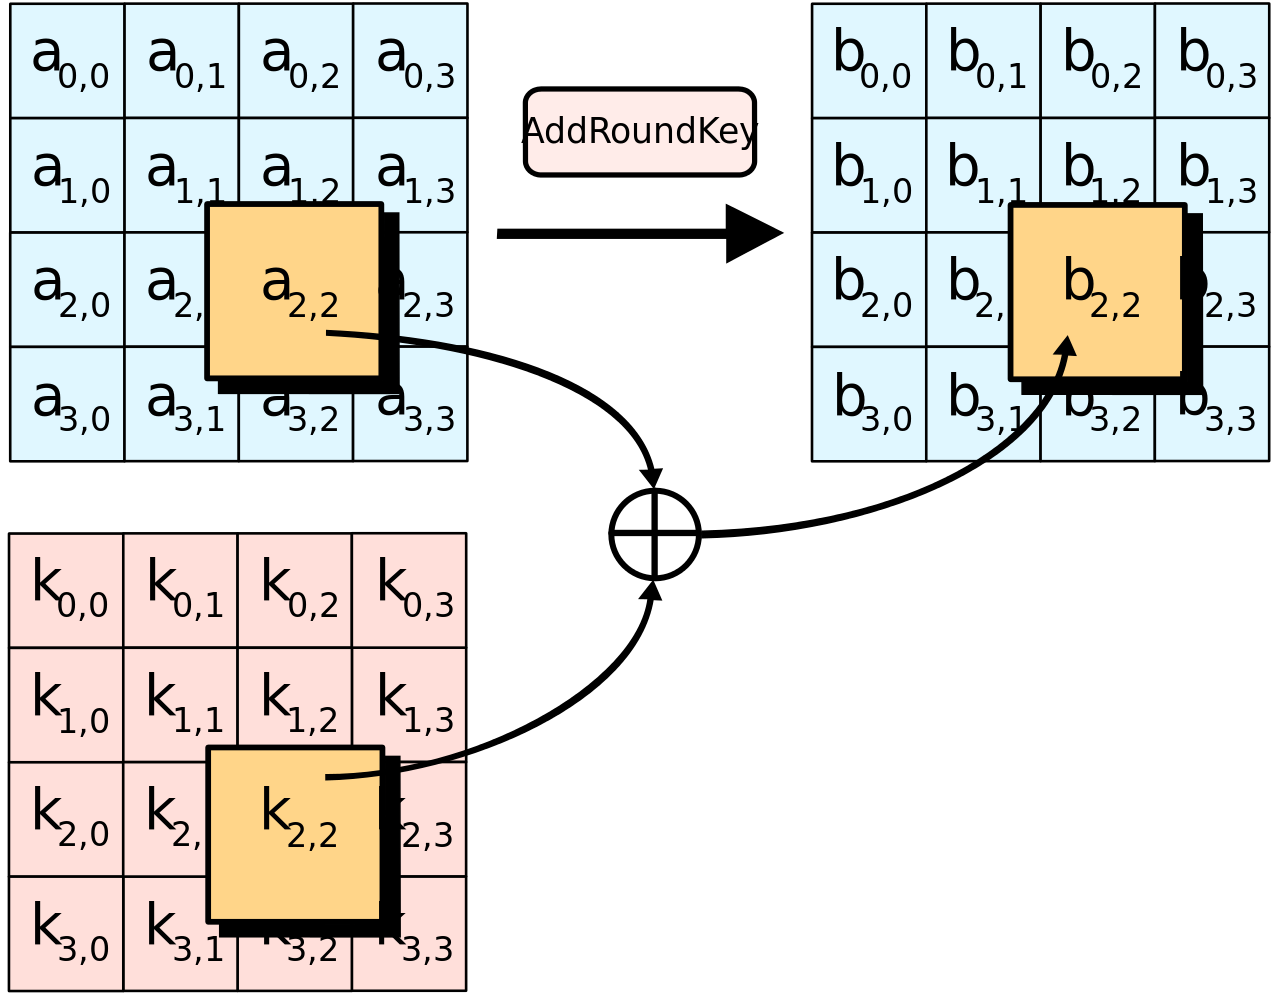
\includegraphics[width=0.45\textwidth]{images/Lec8/AddRoundKey.png}
	\caption{AddRoundKey.}
	\label{fig:addroundkey}
\end{wrapfigure}
\subsubsection{SubBytes}
A fixed non-linear substitution, called S-box, is applied to each byte of the block. Given a byte in hexadecimal notation, the first digit is used to select a row and the second one to select a columns. For examle 0x25 would be the third row (2) and the sixth column (5), giving 0x3f. The standard AES S-box is reported in Figure \ref{fig:sbox}. This S-box hs been obtained by taking, for each byte, its multiplicative inverse in the field. This can bencomputed efficiently via an algorithm that we will see later on, noted b$_7$,...,b$_0$, and applying the affine transformation.
\[b_i=b_i \oplus b_{i+4 \ mod8}\oplus b_{i+5 \ mod8}\oplus b_{i+6 \ mod8}\oplus b_{i+7 \ mod8}\oplus c_i\]
with $c_i$ representing the i-th bit of 01100011.\\

\begin{wrapfigure}[4]{r}{0.47\textwidth}
	%\centering
	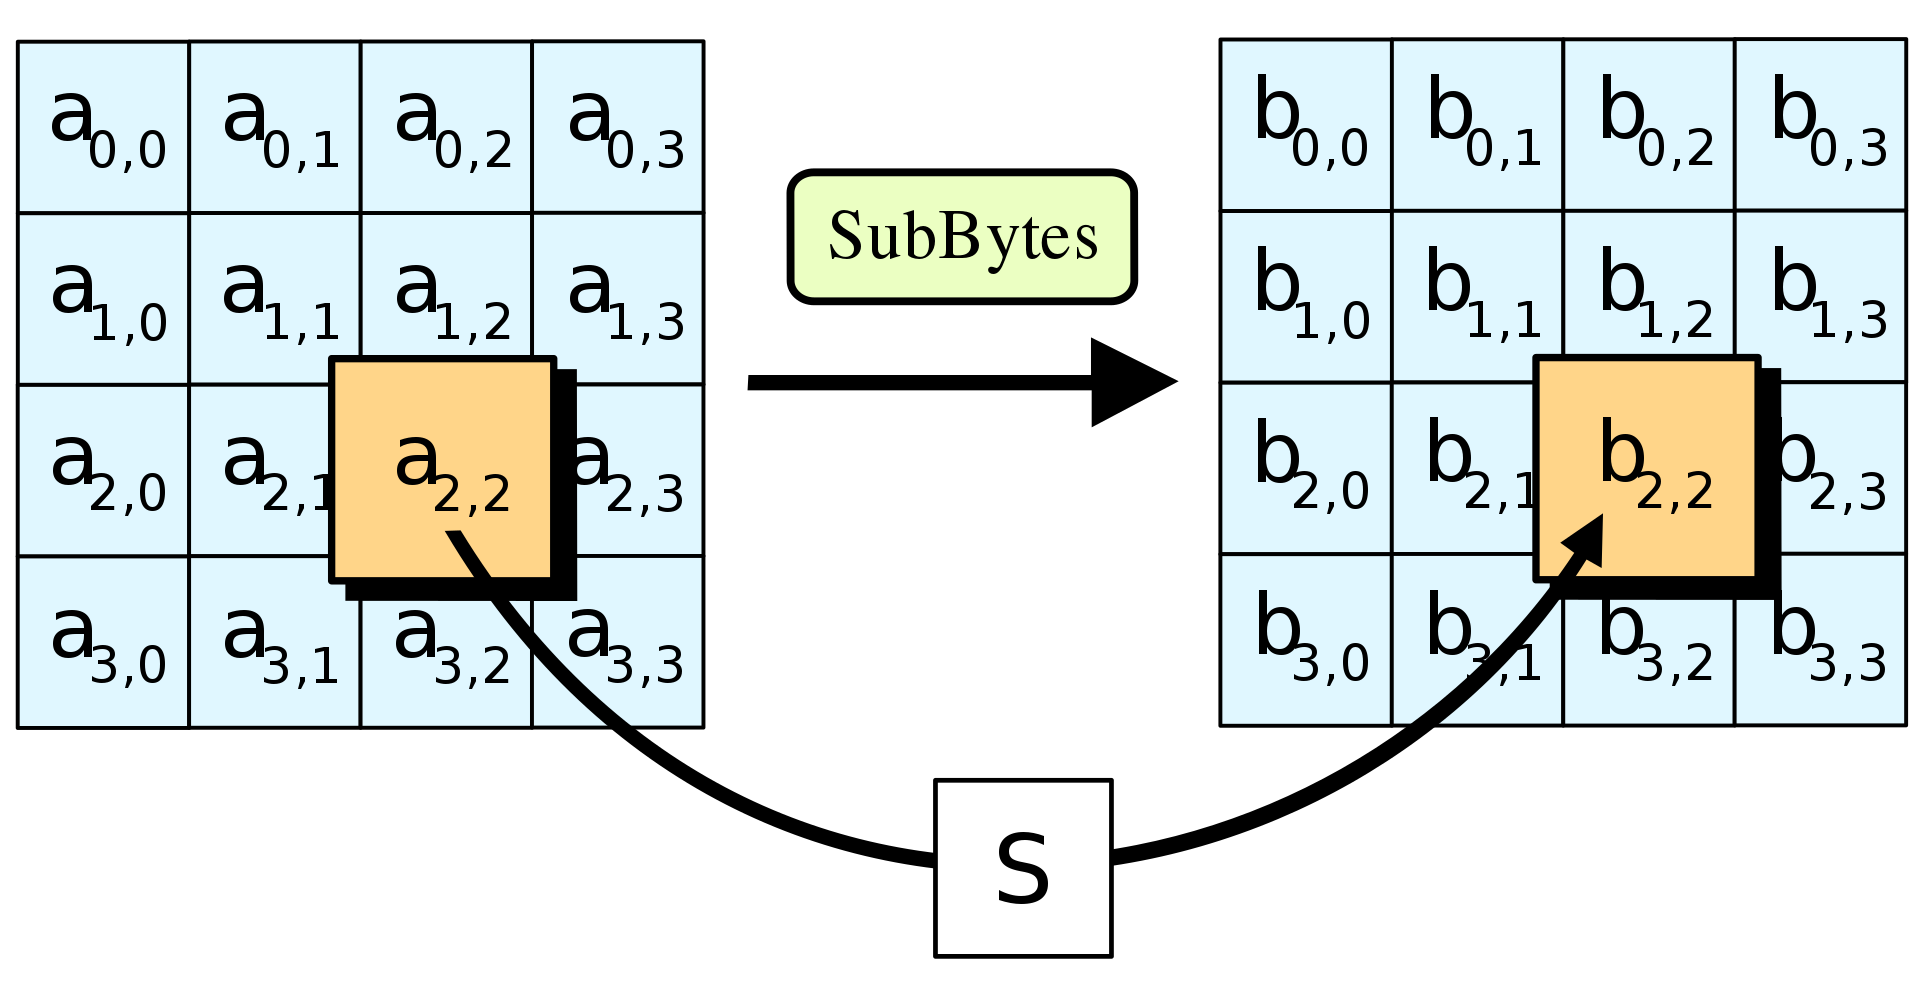
\includegraphics[width=0.45\textwidth]{images/Lec8/SubBytes.png}
	\caption{SubBytes.}
	\label{fig:subbytes}
\end{wrapfigure}

Using multiplicative inverses is known to give non-linear properties, while the affine transformation complicates the attempt of algebraic reductions.
\vspace{35mm}
\begin{figure}[H]
	\centering
	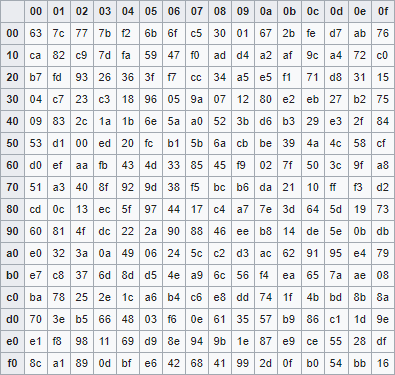
\includegraphics[scale=0.7]{images/Lec8/sbox1.png}
	\caption{Standard AES S-box.}
	\label{fig:sbox}
\end{figure}

\begin{wrapfigure}[0]{r}{0.47\textwidth}
	%\centering
	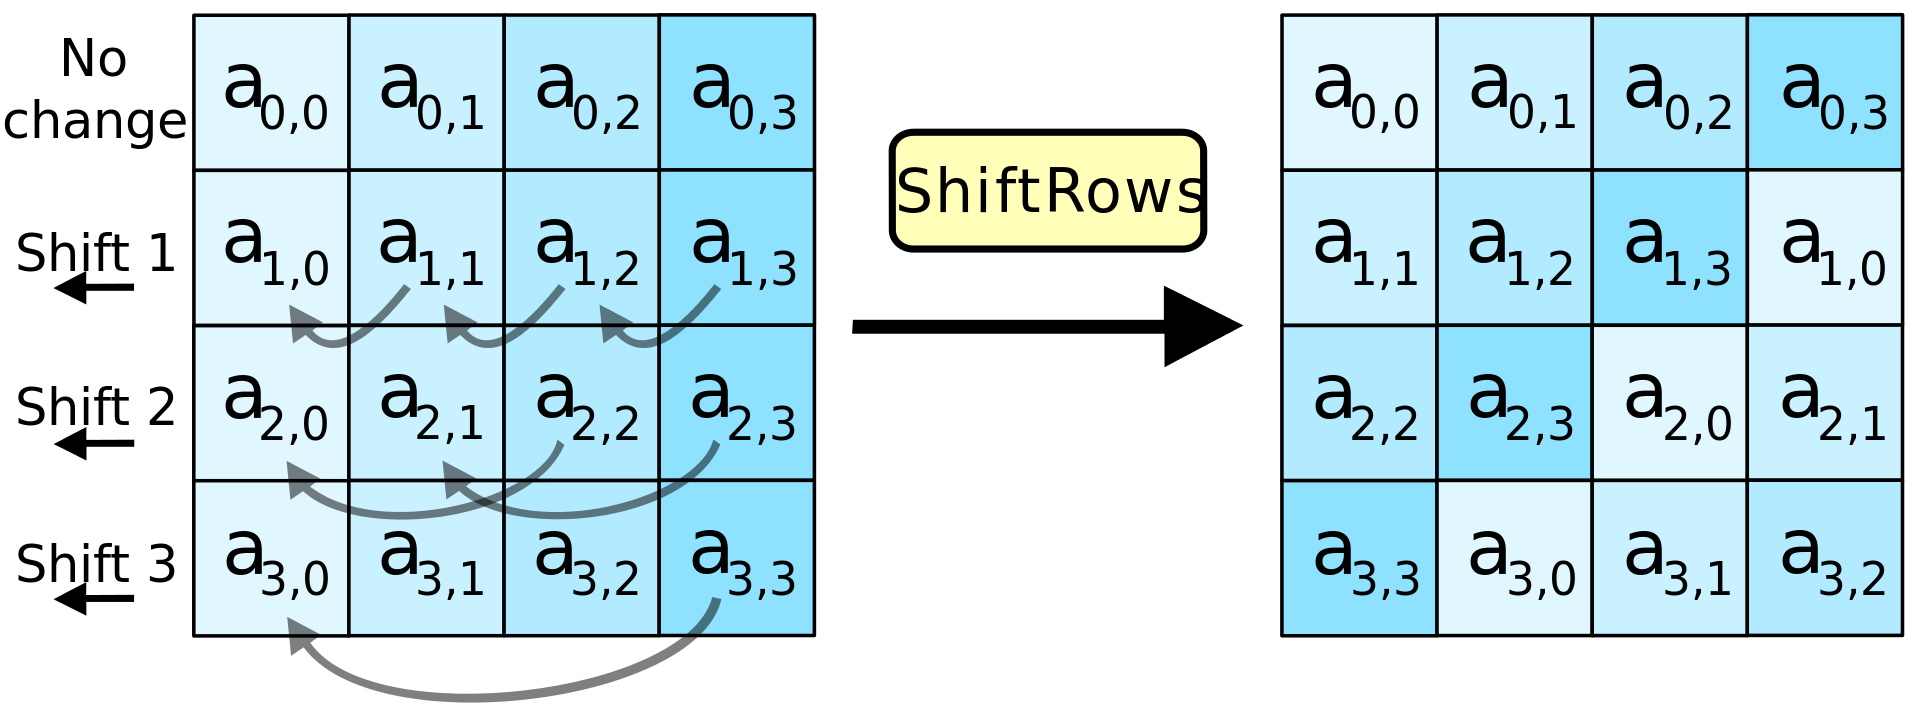
\includegraphics[width=0.45\textwidth]{images/Lec8/ShiftRows.png}
	\caption{ShiftRows.}
	\label{fig:shiftrows}
\end{wrapfigure}


\subsubsection{ShiftRows}
Rows of the block matrix are shifted to\\the left by 0,1,2,3 respectively. The shift\\is circular.
\vspace{5mm}
\subsubsection{MixColumns}
Column of the block matrix are multiplied by the following matrix:

\begin{center}	
	\[ \left[ \begin{array}{c}
	c_0 \\
	c_1 \\
	c_2 \\
	c_3
	\end{array} \right]
	=
	\left[ \begin{array}{cccc}
	2 & 3 & 1 & 1 \\
	1 & 2 & 3 & 1 \\
	1 & 1 & 2 & 3 \\
	3 & 1 & 1 & 2 \\
	\end{array} \right]
	\left[ \begin{array}{c}
	c_0 \\
	c_1 \\
	c_2 \\
	c_3
	\end{array} \right]
	\]
\end{center}
For example, the first byte of each column is computed as \[2c_0\oplus 3c_1\oplus c_2\oplus c_3\]

\begin{wrapfigure}[11]{l}{0.47\textwidth}
	%\centering
	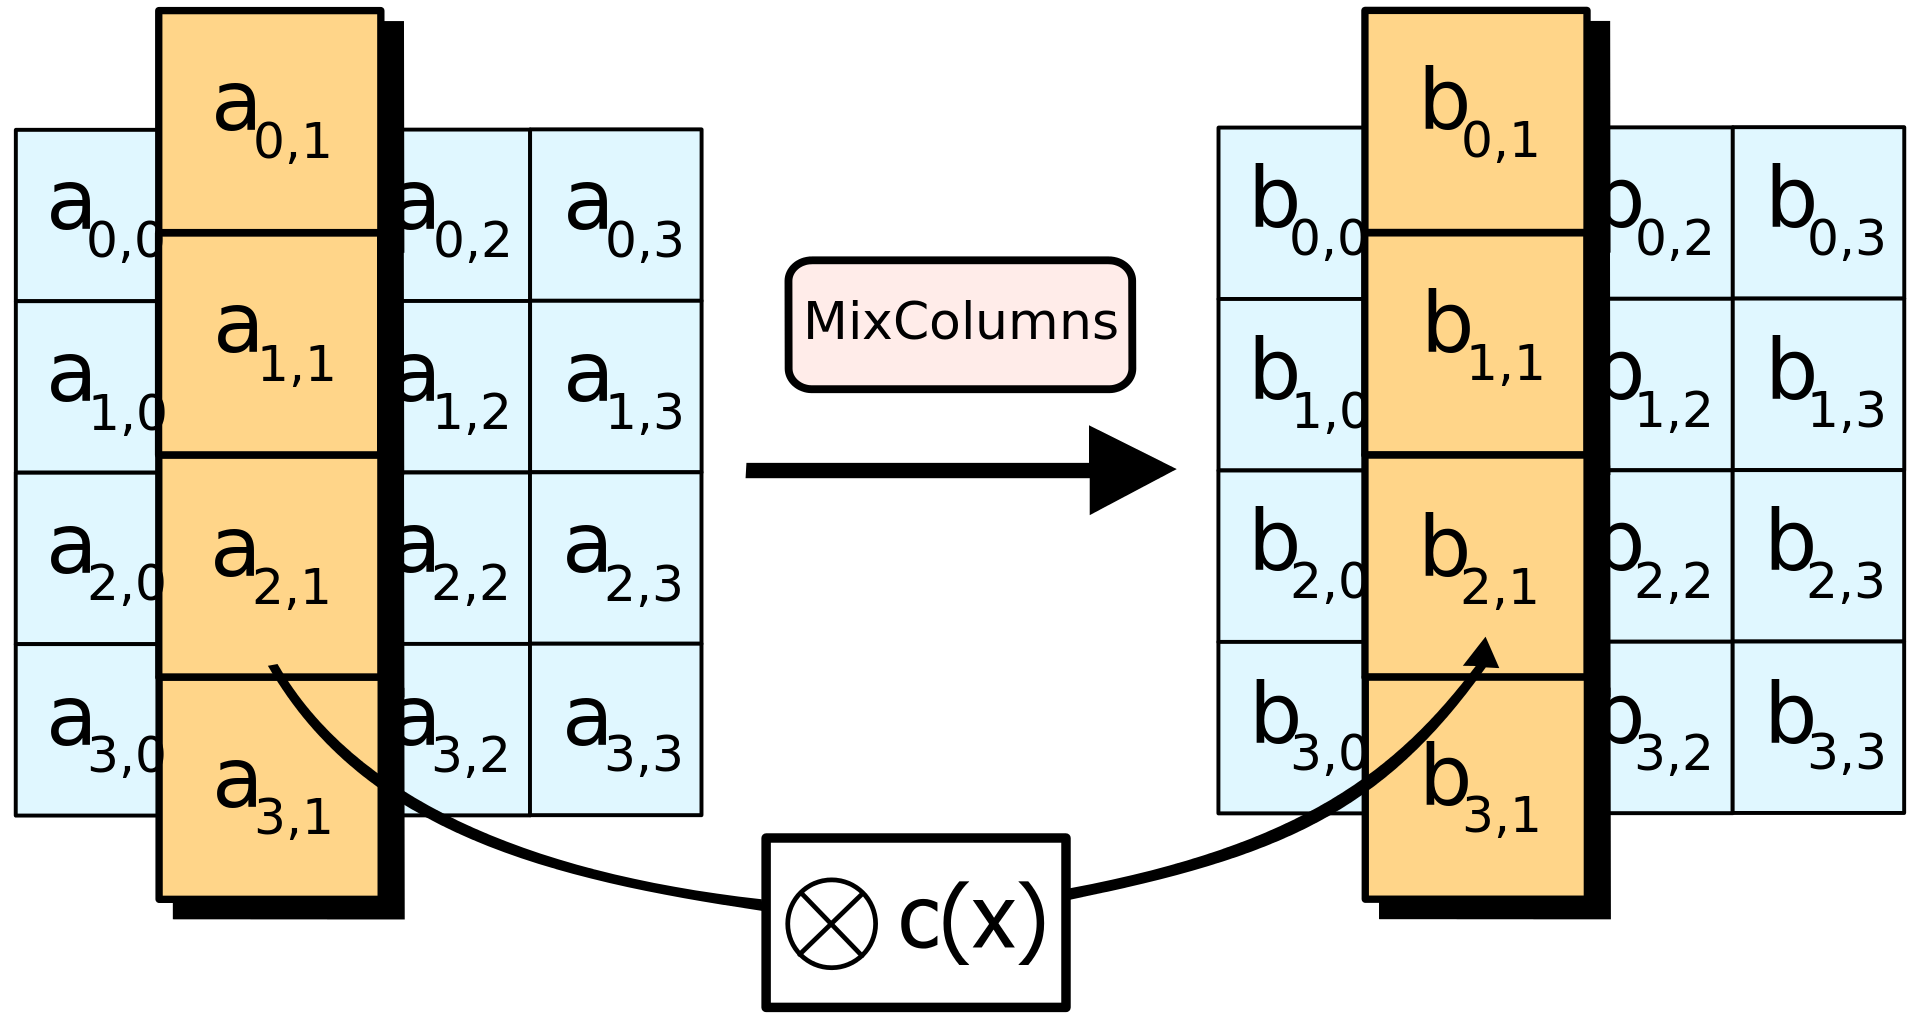
\includegraphics[width=0.45\textwidth]{images/Lec8/MixColumns.png}
	\caption{MixColumns.}
	\label{fig:mixcolumns}
\end{wrapfigure}
We have mentioned that AES uses round keys in the AddRoundKey step. These keys are in fact derived from the initial AES key as follows. Keys are represented as arrays of words of 4 bytes. So, for example, a 128 bits key will be 4 words of 4 bytes, i.e., 16 bytes.\\
This is expanded into an array of size 4*(Nr+1), where Nr is the number of rounds. In this way we obtain 4 different words of key for each round.

Here is the overall scheme for AES assuming that variable state is initialized with the 4$\times$4 matrix of the plaintext (see above) and w[] has been initialized by key expansion.

\begin{python}
	AddRoundKey(state, w[0,3])
	
	for round in range(1,Nr):
		SubBytes(state)
		ShiftRows(state)
		MixColumns(state)
		AddRoundKey(state, w[round*4,round*4+3])
	
	SubBytes(state)
	ShiftRows(state)
	AddRoundKey(state, w[Nr*4,Nr*4+3])
\end{python}

At each round a new key is generated.
\newpage
The AES decryption is compute applying inverse operations:
\begin{python}
	AddRoundKey(state, w[Nr*4,Nr*4+3])
	
	for round in range(Nr-1,0,-1):
		InvShiftRows(state)
		InvSubBytes(state)
		AddRoundKey(state, w[round*4,round*4+3])
		InvMixColumns(state)
		
	InvShiftRows(state)
	InvSubBytes(state)
	AddRoundKey(state, w[0,3])
\end{python}

InvSubBytes is computed by using the inverse substitution of the S-Box in Figure \ref{fig:inversesbox}.

\begin{figure}[H]
	\centering
	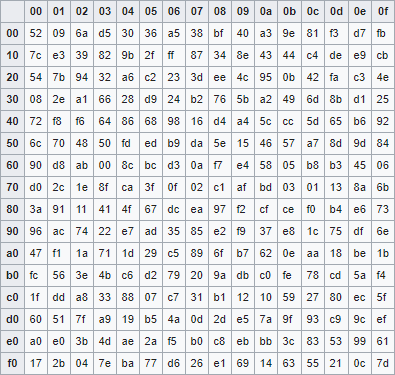
\includegraphics[scale=0.7]{images/Lec8/inversesbox.png}
	\caption{Standard AES inverted S-box.}
	\label{fig:inversesbox}
\end{figure}

InvMixColumns is given by the following operation:

\begin{center}	
	\[ \left[ \begin{array}{c}
	c_0 \\
	c_1 \\
	c_2 \\
	c_3
	\end{array} \right]
	=
	\left[ \begin{array}{cccc}
	0e & 0b & 0d & 09 \\
	09 & 0e & 0b & 0d \\
	0d & 09 & 0e & 0b \\
	0b & 0d & 09 & 0e \\
	\end{array} \right]
	\left[ \begin{array}{c}
	c_0 \\
	c_1 \\
	c_2 \\
	c_3
	\end{array} \right]
	\]
\end{center}

The algorithm for decryption is written in a form similar to the one for encryption but operations are not in the same order. It can, in fact, become the very same algorithm by noticing that SubBytes and ShiftRows commute. It does not matter if we first apply the byte-wise substitution or if we first shift the rows. The final result will be the same. Of course, the same holds for the inverse transformations InvMixColumns(state roundKey) = InvMixColumns(state) InvMixColumns(roundKey). This allows for inverting the two functions, provided that InvMixColumns is applied to all the round keys.

Call dw the array containing the round keys transformed via InvMixColumns. The final decryption algorithm is:
\begin{python}
	AddRoundKey(state, w[Nr*4,Nr*4+3])
	
	for round in range(Nr-1,0,-1):
	InvSubBytes(state)
	InvShiftRows(state)
	InvMixColumns(state)
	AddRoundKey(state, w[round*4,round*4+3])
	
	InvSubBytes(state)
	InvShiftRows(state)
	AddRoundKey(state, w[0,3])
\end{python}

This is exactly the sam as the one for encryption, but with the inverse functions. Having the same algorithm for encryption and decryption simplifies a lot implementations, especially if they are done in hardware.

\begin{exercise}
	Using the algorithm with a,b and p, multiply (x$^4$+x$^3$+1)$\times$(x$^5$+1)
	
	\begin{table}[H]
		\centering
		\begin{tabular}{|c|c|c|}
			\hline
			\textbf{a} & \textbf{b} & \textbf{p} \\ \hline
			11001 & 100001 & 0\\
			110010 & 10000 & 0$\oplus$11001=11001\\
			1100100 & 1000 & 11001\\
			11001000 & 100 & 11001\\
			110010000 & 10 & 11001\\
			(XOR) 10001011 & 10 & 11001\\
			100010110 & 1 & 11001\\
			(XOR)1101 & 1 & 11001\\
			11010 & & 11001$\oplus$1101=10100\\
			\hline
		\end{tabular}
	\end{table}
	In two steps we had a number longer than 8 bits, so we had to xor it with the irreducible polynomial.
\end{exercise}

\chapter*{Lecture 9}
As we said on the previous lecture, the security of AES also depends on the number of rounds: by 2006 the best known attack were on 7 rounds for 128-bits keys, 8 round for 192-bits keys and 9 rounds for 256-bits keys.

\section*{Block cipher modes}
When using block ciphers we have to face the problem of encrypting plaintexts that are longer than the block size. We then adopt a mode of operation, i.e., a scheme that repeatedly applies the block cipher and allows for encrypting a plaintext of arbitrary size. This can be apply to any block cipher (AES, etc.), so encryption and decryption will depend on the chosen one.


\subsubsection{Electronic CodeBlock mode (ECB)}
This is the simplest mode, it is what we have done so fare with classic ciphers: the plaintext X is split into blocks x$_1$,..,x$_n$ whose size is exactly the same as the size of the cipher block. Each block is then encrypted independently using the fixed key k.

\begin{example}
	An example is a substitution cipher applied to letters. What we do is to split the plaintext into single letters that are encrypted independently.
	\begin{figure}[H]
		\centering
		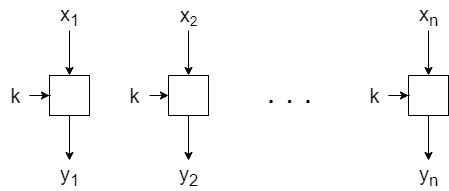
\includegraphics[scale=0.6]{images/Lec4/blockciphers.png}
		\caption{Example of ECB encryption with substitution cipher.}
		\label{fig:exampleECBEnc}
	\end{figure}
	Decryption operation is done by reversing the scheme.
	\begin{figure}[H]
		\centering
		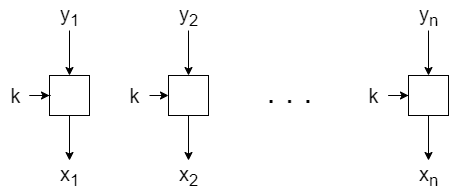
\includegraphics[scale=0.6]{images/Lec9/ECBDec.png}
		\caption{Example of ECB decryption with substitution cipher.}
		\label{fig:exampleECBDec}
	\end{figure}
\end{example}

Pros of this approach:
\begin{itemize}
	\item this scheme has the advantage of being very simple and fast, especially on multi-core computers;
	\item each single encryption/decryption can be performed independently. 
\end{itemize}

But there are a lot of cons:
\begin{itemize}
	\item the security of the scheme is poor;
	\item as monoalphabetic classic ciphers equal plaintext blocks are encrypted in the same way;
	\item this allows for the construction of a code-book mapping ciphertexts back to plaintexts;
	\item often in practice part of a plaintext is fixed due (for example) to the message format. E.g., a mail starting with "Dear Alice, ..";
	\item if we know a part of the plaintext, we know how the blocks containing that part are encrypted;
	\item we can use this information to decrypt other parts of the message, whenever we see the same block occurring;
	\item complete absence of integrity, an attacker in the middle might duplicate, swap, eliminate encrypted blocks and this would correspond to a plaintext where the same blocks are duplicated, swapped, eliminated;
	\item with information about the format of the plaintext, an attacker might be able to obtain a different meaningful plaintext;
	\item how critical is this attack depends on the applications, but it is not a good idea to leave such an easy opportunity.
\end{itemize}
	
In Figure \ref{fig:exampleImageECB} we can see that large areas with the same uniform colour maintain the same pattern when encrypted using ECB.

The weakness of this method is that we use always the same key.
\begin{figure}[H]
	\centering
	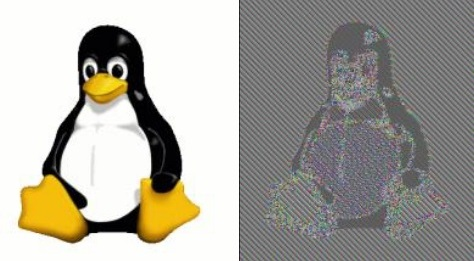
\includegraphics[scale=0.7]{images/Lec9/imageECB.png}
	\caption{Image encrypted with ECB.}
	\label{fig:exampleImageECB}
\end{figure}

\subsubsection{Cipher Block Chaining mode (CBC)}
This mode solves or mitigates all the previous issues of ECB, it prevents equal plaintexts to be encrypted the same way and, at the time, it provides a higher degree of integrity, even if it is not yet satisfactory on this aspect. The idea is to "chain" encryption of blocks using the previous encrypted block. The first block is chained with a special number called \textbf{Initialization Vector} (IV) that can be sent in clear but has to be random and has to change every time (for every cipher mode).

Encryption and decryption schemas are represented in Figure \ref{fig:encCBC} and in Figure \ref{fig:decCBC}.
\begin{figure}[H]
	\centering
	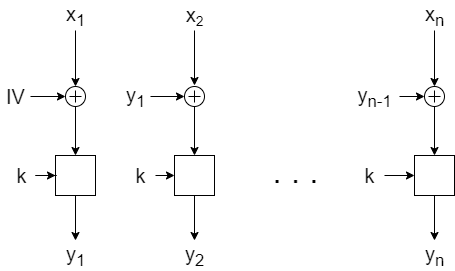
\includegraphics[scale=0.55]{images/Lec9/encCBC.png}
	\caption{Encryption schema of CBC.}
	\label{fig:encCBC}
\end{figure}

\begin{figure}[H]
	\centering
	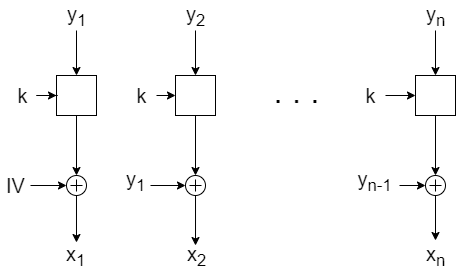
\includegraphics[scale=0.55]{images/Lec9/decCBC.png}
	\caption{Decryption schema of CBC.}
	\label{fig:decCBC}
\end{figure}

Pros of this method:
\begin{itemize}
	\item as mentioned above, CBC never encrypts the same plaintext block in the same way, preventing the code-block attack;
	\item integrity is improved, but is not yet satisfactory. If an attacker swaps, duplicates or eliminates encrypted blocks, this will result in at least one corrupted plaintext block (for example, changing y$_1$ propagates to y$_2$). Notice however that this might be unnoticed at the application level and, again, we cannot leave to the application the whole task of checking integrity of decrypted messages (the application might not check $y_1$). 
\end{itemize}

The cons are:
\begin{itemize}
	\item using xor introduces a new weakness: the attacker manipulating one bit of an encrypted block y$_i$ obtains that the same bit of plaintext x$_{i+1}$ is also manipulated (because we use a xor);
	\item at the same time x$_i$ is corrupted;
	\item we cannot do parallel computations.
\end{itemize}

\begin{exercise}
	Write the expression for CBC encryption and decryption of the i-th block and show, formally, that D$_k^{CBC}$(E$_k^{CBC}$(x$_i$))=x$_i$. To avoid defining a special expression for y$_1$, you can let y$_0$=IV.
	
	E$_k^{CBC}$(x$_i$) = E$_k$(x$_i \oplus$y$_{i-1}$);\\
	D$_k^{CBC}$(y$_i$) = D$_k \oplus$y$_{i-1}$.
	
	\setcounter{equation}{0}
	\begin{align}
		D_k^{CBC}(E_k^{CBC}(x_i)) &= D_k^{CBC}(E_k(x_i \oplus y_{i-1}))\\
		&= D_k(E_k(x_i \oplus y_{i-1})) \oplus y_{i-1}\\
		&= (x_i \oplus y_{i-1}) \oplus y_{i-1}\\
		&= x_i \oplus (y_{i-1} \oplus y_{i-1})\\
		&= x_i
	\end{align}
\end{exercise}

\subsubsection{Output Feedback mode (OFB)}
We now see two modes of operation that "transform" block ciphers into \textbf{stream ciphers}. The general idea is to use the block cipher to generate a complex key stream. Encryption is then performed by just XORing the plaintext blocks with the keys of the stream. Intuitively, this is like one-time-pad with a generated key stream, the more the stream is close to a random stream, the more the cipher will be close to a perfect one.

The encryption and decryption schemas of OFB are represented in Figure \ref{fig:encOFB} and in Figure \ref{fig:decOFB}.

Notice that the key generation is completely independent of the plaintext and ciphertext. In fact, it is possible to generate the key stream offline, having key k, and perform encryption later on, when necessary.
\begin{figure}[H]
	\centering
	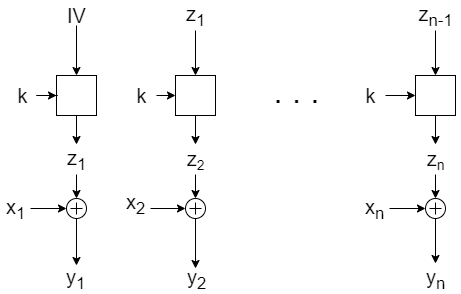
\includegraphics[scale=0.55]{images/Lec9/encOFB.png}
	\caption{Encryption schema of OFB.}
	\label{fig:encOFB}
\end{figure}

\begin{figure}[H]
	\centering
	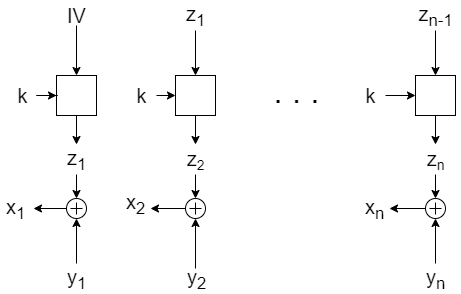
\includegraphics[scale=0.55]{images/Lec9/decOFB.png}
	\caption{Decryption schema of OFB.}
	\label{fig:decOFB}
\end{figure}

Decryption simply consists of "swapping the arrows" when performing the XOR: ciphertexts are XORed with the key stream to recover the plaintexts.

The generation of the key stream is CBC encryption of a zero plaintext, it is thus possible to reuse CBC implementations to compute it. Notice also that the plaintext blocks can be smaller than the size of the block cipher. In that case it is possible to use part of the key and use the remaining part for the next block. For example, if the size of the block is 128 bits (like in AES), and we have to encrypt a single byte, we have that one key can be slit into 128/8=16 keys of 8 bits, each used to encrypt a single byte.

Pros of this method:
\begin{itemize}
	\item This cipher is very efficient (key can be precomputed using CBC) and allows for the encryption of streams of plaintexts;
	\item key stream is generated through a block cipher which makes it very hard to be predicted
\end{itemize}  

The cons:
\begin{itemize}
	\item this stream cipher is synchronous since the key stream is independent of the plaintext;
	\item as a consequence, if we reuse the same IV with the same key, we obtain the same key stream. Since encryption is XOR, attacking the cipher is the same as attacking one-time-pad when the key is used more than once. Thus the IV must be changed any time we encrypt a new message under the same key k;
	\item moreover, an attacker in the middle can arbitrarily manipulate bits of the plaintext by swapping the corresponding bits in the ciphertext. No decrypted blocks will be corrupted. For this reason this mode should only be used in applications where integrity of the exchanged message is not an issue or is achieved via additional mechanism. An example could be satellite transmissions where an attacker is extremely unlikely to be in the middle and confidentiality is the only issue;
	\item in this setting, absence of integrity becomes useful to avoid noise propagation: an error on one bit will only affect one bit of the plaintext.
\end{itemize}

\subsubsection{Counter mode (CTR)}
It is a variation of OFB where the IV is a random number (nounce) and a counter. The random number can be sent in clear (bit should change at any new stream generation) and the counter changes value during the stream generation. It is widely used in practice.

\begin{figure}[H]
	\centering
	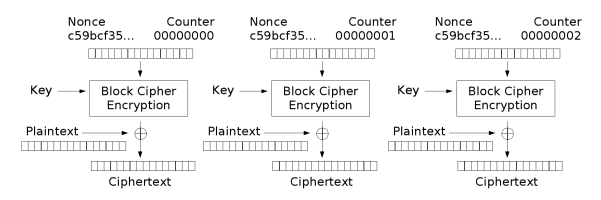
\includegraphics[scale=0.8]{images/Lec9/encCTR.png}
	\caption{Encryption schema of CTR.}
	\label{fig:encCTR}
\end{figure}

\subsubsection{Cipher Feedback mode (CFB)}
This mode mitigates the problems of OFB by making the key stream dependent on the previous encrypted element. To preserve the ability of encrypting plaintexts of size less than or equal to the size of the block of the cipher (a single byte for example), this mode uses shift register that is updated at each step. The register is shifted to the left the number of bits of previous ciphertext (8 for a byte), and such a ciphertext is copied into the rightmost bit of the register.

Encryption and decryption schemas are reported in Figure \ref{fig:encCFB} and in figure \ref{fig:decCFB}.

In decryption, as for OFB, the key stream is generated and XORed to the ciphertexts to reconstruct the plaintexts.
\begin{figure}[H]
	\centering
	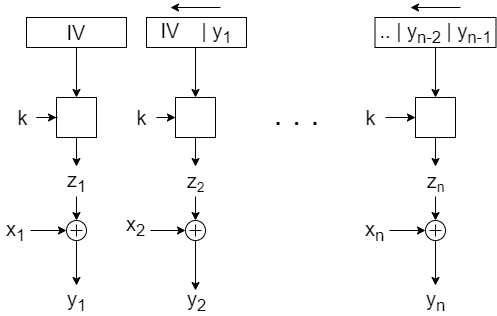
\includegraphics[scale=0.55]{images/Lec9/encCFB.png}
	\caption{Encryption schema of CFB.}
	\label{fig:encCFB}
\end{figure}

\begin{figure}[H]
	\centering
	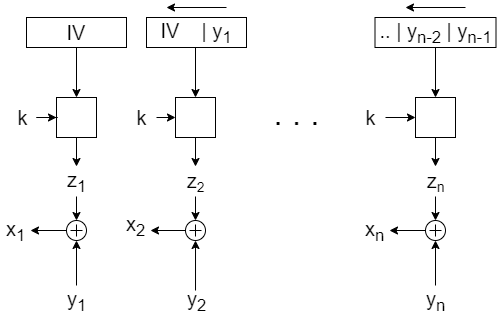
\includegraphics[scale=0.55]{images/Lec9/decCFB.png}
	\caption{Decryption schema of CFB.}
	\label{fig:decCFB}
\end{figure}

Pros:
\begin{itemize}
	\item this mode provides a higher degree of integrity with respect to OFB: whenever one bit of one ciphertext is modified, the next BSize/CSize plaintexts are corrupted, where BSize is the size of the block of the cipher (128 bytes for example) and CSize is the size of the single ciphertext (8 bits for example);
	\item for example, with AES and 8 bits of plaintext/ciphertext sizes we have 128/8=16 corrupted decryptions;
	\item this number corresponds to the number of left shifts necessary for a ciphertext to exit the shift register.
\end{itemize}

Cons:
\begin{itemize}
	\item this cipher is slower than OFB as it requires the previous ciphertext to compute the next, meaning that parallelization is impossible when encrypting;
	\item moreover, for noisy transmission (satellite, Tv, ..) it has the problem of propagating an error on a single bit over the next BSize/CSize plaintexts, which are completely corrupted.
\end{itemize}

\begin{exercise}
	Encode the plaintext "Two One Nine Two" with AES. The key is "Thats my Kung Fu".
	
	First of all we have to transform the plaintext and the key into a Hex notation, using the ASCII table.
	
	Two One Nine Two $\rightarrow$ \texttt{54 77 6F 20 4F 6E 65 20 4E 69 6E 65 20 54 77 6F}\\
	Thats my Kung Fu $\rightarrow$ \texttt{54 68 61 74 73 20 6D 79 20 4B 75 6E 67 20 46 75}
	
	Writing into matrices we have:
	\begin{center}
		\[P=\left[ \begin{array}{cccc}
			54 & 4F & 4E & 20 \\
			77 & 6E & 69 & 54 \\
			6F & 65 & 6E & 77 \\
			20 & 20 & 65 & 6F \\
		\end{array} \right] \ \ \ \ 
		K=
		\left[ \begin{array}{cccc}
			54 & 73 & 20 & 67 \\
			68 & 20 & 4B & 20 \\
			61 & 6D & 75 & 46 \\
			74 & 79 & 6E & 75 \\
		\end{array} \right]
		\]
	\end{center}

	Now we have to apply Key expansion for 10 rounds as we are using a 128-bits key.
	
	We AddRoundKey, XORing P and K, to do the XOR, we have to transform Hex to binary and then go back to represent the result:
	\begin{center}
		\[\left[ \begin{array}{cccc}
		00 & 3C & 6E & 47 \\
		1F & 4E & 22 & 74 \\
		0E & 08 & 1B & 31 \\
		54 & 59 & 0B & 1A \\
		\end{array} \right]\]
	\end{center}
	At this point we apply SubBytes, a fixed non-linear substitution, called S-Box is applied to each byte of the block.
	\begin{center}
		\[\left[ \begin{array}{cccc}
		63 & EB & 9F & A0 \\
		C0 & 2F & 93 & 92 \\
		AB & 30 & AF & C7 \\
		20 & CB & 2B & A2 \\
		\end{array} \right]\]
	\end{center}

	ShiftRows: rows of the block matrix are shifted to the left by 0,1,2,3 respectively.
	\begin{center}
		\[\left[ \begin{array}{cccc}
		63 & EB & 9F & A0 \\
		2F & 93 & 92 & C0 \\
		AF & C7 & AB & 30 \\
		A2 & 20 & CB & 2B \\
		\end{array} \right]\]
	\end{center}
	
	MixColumns: columns of the block are multiplied by the following matrix:
	
	\begin{center}	
		\[ \left[ \begin{array}{c}
		c_0 \\
		c_1 \\
		c_2 \\
		c_3
		\end{array} \right]
		=
		\left[ \begin{array}{cccc}
		2 & 3 & 1 & 1 \\
		1 & 2 & 3 & 1 \\
		1 & 1 & 2 & 3 \\
		3 & 1 & 1 & 2 \\
		\end{array} \right]
		\left[ \begin{array}{c}
		c_0 \\
		c_1 \\
		c_2 \\
		c_3
		\end{array} \right]
		\]
	\end{center}
	So:
	\begin{center}	
		\[ 
		\left[ \begin{array}{cccc}
		02 & 03 & 01 & 01 \\
		01 & 02 & 03 & 01 \\
		01 & 01 & 02 & 03 \\
		03 & 01 & 01 & 02 \\
		\end{array} \right]
		\times		
		\left[ \begin{array}{cccc}
		63 & EB & 9F & A0 \\
		2F & 93 & 92 & C0 \\
		AF & C7 & AB & 30 \\
		A2 & 20 & CB & 2B \\
		\end{array} \right]		
		=
		\left[ \begin{array}{cccc}
		BA & 84 & E8 & 1B \\
		75 & A4 & 8D & 40 \\
		F4 & 8D & 06 & 7D \\
		7A & 32 & 0E & 5D \\
		\end{array} \right]
		\]
	\end{center}
	At the end we have to XOR again our block with the new key obtained by the Key extension algorithm.
	\begin{center}	
		\[ 
		\left[ \begin{array}{cccc}
		BA & 84 & E8 & 1B \\
		75 & A4 & 8D & 40 \\
		F4 & 8D & 06 & 7D \\
		7A & 32 & 0E & 5D \\
		\end{array} \right]
		\oplus		
		\left[ \begin{array}{cccc}
		E2 & 91 & B1 & D6 \\
		32 & 12 & 59 & 79 \\
		FC & 91 & E4 & A2 \\
		F1 & 88 & E6 & 93 \\
		\end{array} \right]		
		=
		\left[ \begin{array}{cccc}
		58 & 15 & 59 & CD \\
		47 & B6 & D4 & 39 \\
		08 & 1C & E2 & DF \\
		8B & BA & E8 & CE \\
		\end{array} \right]
		\]
	\end{center}

	This is the result of one round, we have to repeat 9 other times to obtain the final matrix.
\end{exercise}

\chapter*{Lecture 10}
In addition to AES there are many other block ciphers in use, such as DES, 3-DES, IDEA, Blowfish and Twofish, RC2, RC5, RC6, ..

\section*{Data Encryption Standard (DES)}
DES is a symmetric key algorithm, the predecessor of AES. It has been published in 1975 and derives from Lucifer (IBM). It has been the most used and implemented cipher in the history and it is currently used in many applications, especially in the triple version. DES major problem is the key-length (only 56 bits) that is considered vulnerable with modern parallel computers.

The first attack known in history goes back to January 1999, when distributed.net and the Electronic Frontier Foundation collaborated to publicly break a DES key in 22 hours and 15 minutes. There are also some analytical results which demonstrate theoretical weakness in the cipher, although they are infeasible to mount in practice.

\begin{wrapfigure}[17]{r}{0.47\textwidth}
	%\centering
	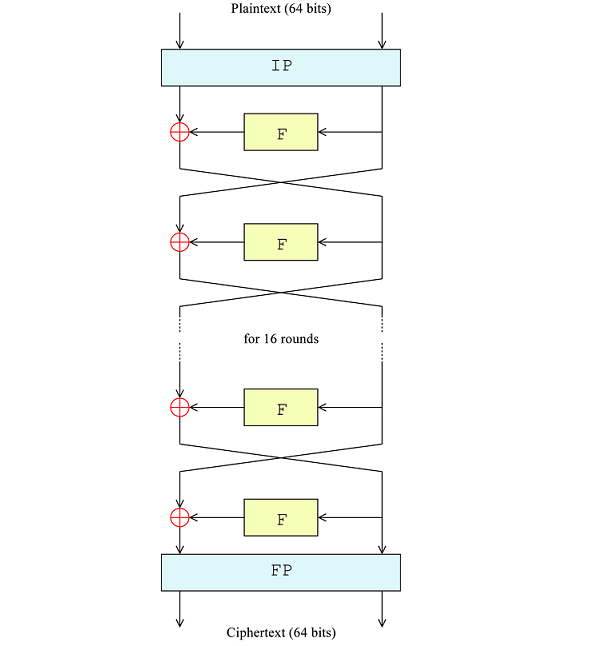
\includegraphics[width=0.45\textwidth]{images/Lec10/DESschema.png}
	\caption{DES encryption schema.}
	\label{fig:desschema}
\end{wrapfigure}
DES takes a fixed-length string of plaintext bits and transforms it through a series of complicated operations into another ciphertext bit string of the same length. The block size is 64 bits an the key length is 56 bits (8 for error correction). It has 16 identical rounds, the encryption starts with an initial permutation (IP) and ends with a final permutation (FP, inverse operation). Before the main rounds, the block is divided into two 32-bit halves and processed alternatively. This criss-crossing is known as the \textbf{Feistel scheme}.

\subsubsection{The Feistel function (F)}
Feistel function consists of different operations: Expansion (from 32 to 48 bits), Key-mixing (key schedule), Substitution S-box (results 32 bits) and Permutation. The schema of the function is represented in Figure \ref{fig:feistel}.

The alternation of substitution from the S-boxes, and permutation of bits from the P-box and E-expansion provides the so-called \textbf{"confusion and diffusion"} (Shannon).

\begin{figure}[H]
	\centering
	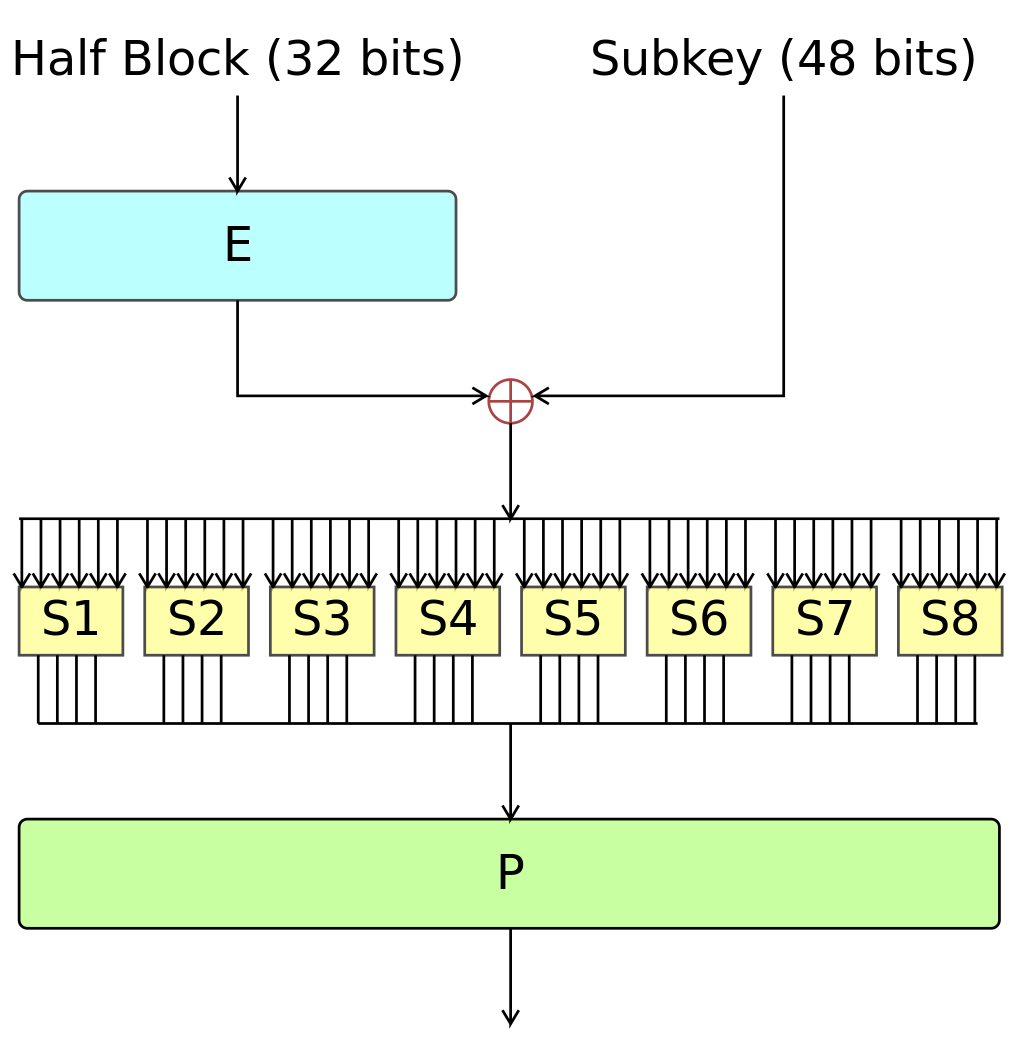
\includegraphics[scale=0.15]{images/Lec10/feistel.png}
	\caption{Feistel function.}
	\label{fig:feistel}
\end{figure}
\textbf{Confusion} is the process that drastically changes data from input to the output (e.g., by translating data through a non-linear table created from the key).

\textbf{Diffusion}: changing a single character of the input will change many characters of the output. 

\section*{International Data Encryption Algorithm (IDEA)}
IDEA was proposed in 1990 as a substitute of DES and it is currently adopted in many applications. It is not based on non-linear substitutions (S-Boxes), confusion and diffusion are obtained by a combination of three operations: xor, sum and multiplication modulo 2$^{16}$. Patent issues have reduced the popularity of this cipher. Compared to other, IDEA performance is not so high.

\section*{Blowfish and Twofish}
Blowfish has been proposed in 1993, it is very fast, compact and simple to implement, with a very highly configurable security: key length is variable up to 448 bits which allows for security/speed trade-off. As DES, it is based on xor and S-Boxes which are not fixed but computed using the cipher itself and the actual key. This key-dependent S-Boxes make brute-forcing particularly expensive: for each key, it is necessary to generate the S-Boxes which takes 522 iterations of the algorithm. Twofish is one of the finalists of AES and "successor" of Blowfish, both ciphers have been developed by Bruce Schneier.

\section*{RC2, RC5, RC6}
They are a family of ciphers developed by Ron Rivest.
\begin{itemize}
	\item RC2 (1987): it is vulnerable to a related-key attack using 2$^{34}$ chosen plaintext;
	\item RC5 (1994): it uses data dependent rotation, it is extremely simple but it requires a complex key-expansion procedure: each round is just two XORs, two sums modulo and two rotations. This cipher is highly configurable on the number of rounds, key-length and word-length, which allows for a sophisticate trade-off between security and performance;
	\item RC6 (derived from RC5): it has been one of the AES finalists. 
\end{itemize}

\section*{3DES}
3DES is a triple iteration of DES, it is implemented, for example, in SSH, TLS/SSL and it is adopted in many commercial applications. Bank circuit and credit card issuers use 3DES in smartcard-based applications and for PIN protection.

The aim of 3DES is to increase key-length. Due to the meet-in-the-middle attack, the triple key of 168 bits is, in fact, equivalent in strength to a key of 112 bits. Meet-in-the-middle is also the reason why 2DES makes no sense: the 112-bits key could be broken in a 2$^{56}$ time/space complexity brute force attack.

One technique is to strengthen ciphers in iteration. All modern ciphers are based on rounds, i.e., repetitions of the same core algorithm. What happens if we iterate a while cipher such as DES or AES? It increases the key length. DES has 56-bit key that is considered weak nowadays. If we iterate the cipher three times using different keys, we obtain (k$_1$, k$_2$, k$_3$) of 168 bits which is too hard to break.

We know that iteration make sense only if the cipher is not idempotent. The following informal argument suggests that modern ciphers are very unlikely to be idempotent. We reason on DES bu the same reasoning would apply to different block ciphers.

\subsubsection{DES is non-idempotent}
DES has a block size of 64 bits, if we list all the 2$^{64}$ possible blocks and we pick one DES key k, the cipher will map each of these blocks into a different block. Since encryption must be invertible, this mapping is injective. Thus, in any block cipher, a key corresponds to a permutation of all the possible plaintext blocks:
\begin{center}
	0 $\rightarrow$ $\rho(0)$\\
	1 $\rightarrow$ $\rho(1)$\\
	2 $\rightarrow$ $\rho(2)$\\
	...\\
	2$^{64}$-1 $\rightarrow$ $\rho(2^{64}-1)$
\end{center}
The number of permutations of 2$^{64}$ elements is 2$^{64}!$ which is enormously big compared to the 2$^{56}$ DEs keys. The way a DES key selects a specific permutation is "complex", otherwise the cipher would be weak. We can thus think of DES keys as selecting a random subset of 2$^{56}$ permutations among the 2$^{64}!$ possible ones.

The probability that the composition of two such permutations is still in this subset (i.e., DES is idempotent) is 2$^{56}$/2$^{64}!$, which is a negligible number. This means that it is really unlikely that 2 iterations of DES (and of any modern block cipher, in fact) correspond to a single encryption under a different key. Thus DES is non-idempotent (there exists also formal proofs).

\section*{Meet-in-the-middle}
Meet-in-the-middle is a known plaintext scenario, i.e., the attacker knows pair of plaintext/ciphertext (X,Y), (X',Y'), (X'',Y''), .., all encrypted under the same key k. The idea is to select one pair, say (X,Y), and try to decrypt Y with all the possible second keys k$_2$. All the resulting values Z are stored into a table together with the key, which is indexed by Z.
\begin{table}[H]
	\centering
	\begin{tabular}{|c|c|}
		\hline
		\textbf{Z} & \textbf{key}\\ \hline
		D$_0$(Y) & 0\\
		D$_1$(Y) & 1\\
		... & ...\\
		D$_{2^{56}-1}$(Y) & 2$^{56}$-1\\ \hline
	\end{tabular}
\end{table} 

Now we try to encrypt under all the possible first keys k$_1$ the plaintext X and we look the obtained value into the table. If we find a match, we test the resulting pair (k$_1$,k$_2$) on all the other plaintext/ciphertext pairs and, if all the tests succeeds, we give it as output.

The computational cost of this attack is 2$^{57}$ steps and 2$^{56}$ space. In fact, first step takes 2$^{56}$ steps to build a table which has 2$^{56}$ entries. Second step takes at most 2$^{56}$ steps to find the right key. We thus have 2$^{56}$ + 2$^{56}$ = 2$^{57}$ steps (vs brute force).

\subsubsection{False keys}
It is very important that, whenever a pair (k$_1$,k$_2$) for (X,Y) is found, it is tested against other pairs (X',Y'). It could be the case, in fact, that a key pair is fine for (X,Y) but it is not the right key pair, this can happen more frequently than expected.

To estimate the number of these false keys we assume that plaintexts are mapped to ciphertext uniformly by the possible keys. i.e., the number of keys mapping X into Y is approximatively the same as the number of keys mapping X into any other ciphertext Y'. This assumption typically holds for any good cipher for which observing Y gives very little information about the plaintext X. Having a non-uniform distribution would imply that the plaintexts
mapped by more keys into Y are more likely than the ones mapped by less keys.

Under these assumptions, we can then estimate the number of false keys as |K|/|C|, i.e., the number of keys divided by the number of ciphertexts which is, for 2DES, 2$^{112}$/2$^{64}$=2$^{48}$. This huge number of possible keys encrypting X into Y can be reduced very quickly by testing keys on more pairs.

The probability that a false key is also OK for (X',Y') is just 1 over the number of all the possible ciphertexts (we have only one good case Y' over all the possible 2$^{64}$ ciphertexts) giving 1/2$^{64}$. Thus, the number of false keys is reduced to 2$^{48}$/2$^{64}$ = 1/2$^{16}$. If we try on one more pair we get 1/2$^{80}$, and so on. In summary, with 3 available pairs of plaintext/ciphertext we can run the attack having a negligible probability of getting a false key.

\subsubsection{Lesson learned}
The cost in time is thus basically the same as the one for a single iteration of DES, for this reason 2DES is never used in practice and, instead, we have a triple iteration known as triple-DES (3DES), this gives a 168-bit triple key (k$_1$,k$_2$,k$_3$).

The meet-in-the-middle attack is still possible in 3DES but it reduces the cost in time to 2$^{112}$ with a table of size 2$^{56}$ entries. The idea is to build the table by decrypting Y under all k$_3$ and then try all the pairs (k$_1$,k$_2$).

\begin{exercise}
	Encode message M=(3,2) using the Hill cipher with key matrix
	\[K=
	\left[ \begin{array}{cc}
		3 & 1 \\
		1 & 2 \\
	\end{array} \right]
	\]
	Decode the found encrypted message.
	
	\[E_k(3,2) = (3,2) \times 
	\left[ \begin{array}{cc}
		3 & 1 \\
		1 & 2 \\
	\end{array} \right] \text{mod}26 = (9+2,3+4) \text{mod}26 = (11,7)
	\]
	Decryption:
	\[K^{-1} = \text{det}^{-1}(K)
	\left[ \begin{array}{cc}
		2 & -1 \\
		-1 & 3 \\
	\end{array} \right] \text{mod}26 =
	\text{det}^{-1}(K)
	\left[ \begin{array}{cc}
		2 & 25 \\
		25 & 3 \\
	\end{array} \right] \text{mod}26 
	\]
	\[
	\text{det}(K)=(6-1) \text{mod}26=5
	\]
	\[\text{det}^{-1}(K)=21, (21\times 5) \text{mod}26 =1\]
	\[
	K^{-1} =
	21
	\left[ \begin{array}{cc}
	2 & 25 \\
	25 & 3 \\
	\end{array} \right] \text{mod}26 =
	\left[ \begin{array}{cc}
		42 & 525 \\
		525 & 63 \\
	\end{array} \right] \text{mod}26 = 
	\left[ \begin{array}{cc}
	16 & 5 \\
	5 & 11 \\
	\end{array} \right]
	\]
	
	\[D_k(11,7) = 
	(11,7)
	\left[ \begin{array}{cc}
	16 & 5 \\
	5 & 11 \\
	\end{array} \right]\text{mod}26= (176+35, 55+77) \text{mod}26 = (211, 132) \text{mod}26 = (3,2)
	\]
\end{exercise}

\chapter*{Lecture 11}
All the ciphers we have studied so far use the same key K both for encryption and decryption, this implies that the source and the destination of the encrypted data have to share K. For this reason, this kind of ciphers are also known as symmetric-key ciphers.

\begin{wrapfigure}[12]{r}{0.47\textwidth}
	%\centering
	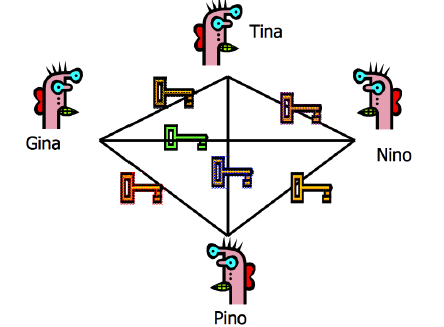
\includegraphics[width=0.45\textwidth]{images/Lec11/simmkeys.png}
	\caption{Symmetric key graph.}
	\label{fig:simmkeys}
\end{wrapfigure}

It becomes problematic if we want cryptography to scale to big systems with many users willing to communicate securely. Unless we have a centralized service to handle keys, for N users, this would require the exchange of N(N-1)/2 keys, O(N$^2$). From another point of view, this is a complete graph.
\begin{example}
	If we have N=4, we would have $\frac{4\times 3}{2}=6$ channels and 6 pairs of symmetric keys.
\end{example}

Symmetric key ciphers make sense until we have a reasonable number of users.

For example in a LAN with 1000 users, we would have $\approx500000$ keys. these keys should be pre-distributed to users in a secure way (e.g., offline) but this is totally impractical and would never scale on a wide-area network such as the Internet.

\begin{wrapfigure}[11]{l}{0.47\textwidth}
	%\centering
	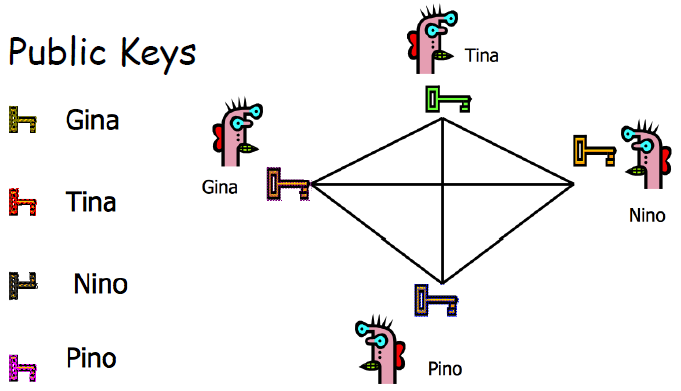
\includegraphics[width=0.45\textwidth]{images/Lec11/publickeys.png}
	\caption{Public keys idea.}
	\label{fig:publickeys}
\end{wrapfigure}

To overcome this problem, in 1976, Whitfield Diffie and Martin Hellman proposed the asymmetric-key ciphers. The idea is the following: a user A has one encrypting and one decrypting key. They are different but correlated (this is why they are called asymmetric). The encrypting key is public, the decrypting key is a secret, known only by A.

The public key is published in a public list and is known by everybody, even the attacker. Public and private keys are correlated but the knowledge of the public key does not give any information about the private key.

A schema of public key cryptography is shown in Figure \ref{fig:asymenc}. 
\begin{figure}[H]
	\centering
	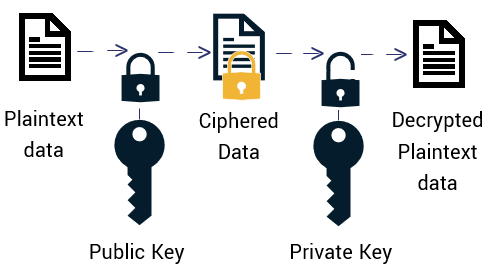
\includegraphics[scale=0.65]{images/Lec11/asymenc.png}
	\caption{Public key encryption schema.}
	\label{fig:asymenc}
\end{figure}

We define the public key of A with \textbf{PK$_A$} and the secret key of A with \textbf{SK$_A$}. If B wants to send a message to A, he sends E$_{PK_A}$(M), when A receives the messages, he decrypt it as D$_{SK_A}$(E$_{PK_A}$(M)).

Encryption and decryption algorithms are defined such that D$_{SK_A}$(E$_{PK_A}$(M)) = M holds.

\begin{definition}
	An \textbf{asymmetric-key cipher} is a quintuple (P,C,K$_S\times$K$_P$,E,D) with E:K$_P\times$P$\rightarrow$C and D:K$_S\times$C$\rightarrow$P and such that:
	\begin{itemize}
		\item it is computationally easy to generate a key-pair (SK,PK) in K$_S\times$K$_P$;
		\item it is computationally easy to compute y=E$_{PK}$(x);
		\item is is computationally easy to compute x=D$_{SK}$(y).
	\end{itemize}
\end{definition}

As said before, D$_{SK}$(E$_{PK}$(x))=x. It is computationally infeasible to to compute SK knowing PK and y. It is also infeasible to compute D$_{SK}$(y) knowing PK and y and without knowing SK.

As encryption is performed under PK while decryption under SK, the decryption key is now different from the encryption key.

What security properties do we have? We achieve secrecy because the attacker is not able to decrypt the message as it doesn't have the secret key SK. On the other hand we cannot assure authentication, everybody can send a message to A saying it is B (with symmetric keys this does not happen). For this reason we need a digital signature.

\subsubsection{One-way-trap-door functions}
\begin{definition}
	An injective, invertible function is \textbf{one-way} iff:
	\begin{itemize}
		\item y=f(x) is easy to compute;
		\item x=f$^{-1}$(y) is infeasible to compute.
	\end{itemize}
\end{definition}

\begin{definition}
	An injective, invertible family of functions f$_k$ is \textbf{one-way trap-door}, iff given k:
	\begin{itemize}
		\item y=f$_k$(x) is easy to compute;
		\item x=f$_k^{-1}$(y) is infeasible to compute without knowing the secret trap-door S(k) relative to k.
	\end{itemize}
\end{definition}

The trap-door is a hidden way to go back to the preimage x of the function, only knowing the trap-door we can compute f$_k^{-1}$(y).

\section*{The Merkle-Hellman knapsack system}
This cipher has been broken, but still gives an idea of how asymmetric-key ciphers relate to one-way-trap-door functions. It is based on the following NP-complete problem:

\textbf{The subset-sum problem}: Let s$_1$,..,s$_n$ and T be positive integers. s$_i$ are sizes while T is the target. A solution to the subset-sum problem is a subset of (s$_1$,..,s$_n$) whose sum is exactly the target T. Formally, the solution is a binary tuple (x$_1$,..,x$_n$) such that $\sum_{i=1}^{n}$x$_i$s$_i$=T.

\begin{example}
	If sizes are (4,6,3,8,1) and T=11, we have that (0,0,1,1,0) and (1,1,0,0,1) are solutions, since 3+8=11 and 4+6+1=11.
\end{example}

This problem is NP-complete in general, as a consequence, we can easily obtain a one-way function from it.\\
If we define f(x$_1$,..,x$_n$)=$\sum_{i=1}^{n}$x$_i$s$_i$ we have that f is clearly easy to compute but inverting this function amounts to finding (x$_1$,..,x$_n$) from a target T which we know to be infeasible for a big n.

How can we now introduce a secret trap-door to allow us to invert the function? The trick is to start from a specific instance of the problem that it is easy to solve.

We consider special sizes that are super-increasing, i.e., such that s$_i>\sum_{j=1}^{i-1}$s$_j$, for each i>1. This means that any s$_i$ is bigger than the sum of all the previous s$_j$. For example (1,3,5,10) is super-increasing, while (1,3,5,9) is not. In this special case there is a very efficient algorithm to solve the subset-sum problem. The idea is to start from the biggest element s$_n$ and go back to the first one: if s$_i$ fits into T, we pick it (we set x$_i$=1), and we subtract s$_i$ from T. The code for the algorithm is the following:

\begin{python}
	def subsetSum(S,T):			#assumes S is a super-increasing list of integers
		x=[]
		S.reverse()						#reverse the list to start from the biggest
		for s in S:						#iterates on all s_i (from the biggest)
			if s<=T:
				x.append(1) 			#takes the element
				T=T-s							#subtract it from T
			else:
				x.append(0)				#does not take the element
		if T==0:							#solution found
			x.reverse()
			return x						#returns the reversed tuple
		else:
			return []						#no solution found
\end{python}

\subsubsection{The cipher}
\begin{itemize}
	\item We start from a super-increasing problem (s$_1$,..,s$_n$);
	\item we choose a prime \textbf{p}>$\sum_{i=1}^{n}$s$_i$;
	\item we choose a random \textbf{a} such that 1<a<p;
	\item we transform the initial super-increasing problem into $\hat{\text{s}_1},..,\hat{\text{s}_n}$, with $\hat{\text{s}_i}$=as$_i$ mod\textit{p}. Notice that this problem is not super-increasing in general.
\end{itemize}

\begin{example}
	Let (1,2,5,12) be a super-increasing sequence, p=23 and a=6. Compute s$_i$a mod\textit{p}.
	\begin{center}
		(1*6) mod 23 = 6\\
		(2*6) mod 23 = 12\\
		(5*6) mod 23 = 7\\
		(12*6) mod 23 = 3
	\end{center}
	Thus we obtain the sequence (6,12,7,3).
\end{example}

The trap-door is composed of (s$_1$,..,s$_n$), p and a, that are kept secret.\\
The public key is ($\hat{\text{s}_1},..,\hat{\text{s}_n}$).

To encrypt we first have to translate the message from ASCII to binary obtaining x$_1$,..x$_n$ and then we can encrypt it as follows:
\begin{center}
	E$_{PK}$(x$_1$,..,x$_n$) = $\sum_{i=1}^{n}$x$_i\hat{\text{s}_i}$
\end{center}

For example, given the plaintext (1,0,0,1) and the sequence (6,12,7,3) we have E$_{PK}$(1,0,0,1) = 1*6 + 0*12 + 0*7 + 1*3 = 6 + 3 = 9.

The decryption works as follows: D$_{SK}$(y) is the solution of the super-increasing problem (s$_1$,..,s$_n$) with target a$^{-1}$y mod\textit{p}.
\begin{example}
	a$^{-1}$ is 4, since a=6, p=23, 6*4 mod 23 = 1.
	
	Given E$_{PK}$(1,0,0,1) = 9, to decrypt we have to compute the target a$^{-1}$*9 mod\textit{p} = 4*9 mod 23 = 13.
	
	We finally solve the super-increasing problem (1,2,5,12) with target 13 with target 13: subsetSum([1,2,5,12],13) = [1,0,0,1] which gives the initial plaintext (1,0,0,1).
\end{example} 

\begin{exercise}
	Let (2,7,11,21,42,89,180,354) be a super-increasing sequence, p=881 and a=588 (secret key).\\
	Compute the public key s$_i$*a mod\textit{p}.\\
	Then compute the encryption and the decryption of letter "a".
	
	Public key:
	\begin{center}
		2*588 mod 881 = 295\\
		7*588 mod 881 = 592\\
		11*588 mod 881 = 301\\
		21*588 mod 881 = 14\\
		42*588 mod 881 = 28\\
		89*588 mod 881 = 353\\
		180*588 mod 881 = 120\\
		354*588 mod 881 = 236\\
	\end{center}
	So the public key is (295,592,301,14,28,353,120,236).
	
	Letter "a" in binary is (0,1,1,0,0,0,0,1)
	Encrypting it we obtain:\\
	E$_{PK}$(0,1,1,0,0,0,0,1) = 592 + 301 + 236 = 1129.
	
	To decrypt, we need to find a$^{-1}$, it is 442, since 588*442 mod 881 = 1.
	The target is: 442*1129 mod 881 = 372.
	subsetSum([2,7,11,21,42,89,180,354],372) = [0,1,1,0,0,0,0,1] and this is the binary value of letter "a". 
\end{exercise}

\chapter*{Lecture 12}
In the previous lecture we said that to decrypt we use a$^{-1}$y mod\textit{p}. But why?

\begin{proof}
	The correctness of the above cipher can be proved as follows:
	\setcounter{equation}{0}
	\begin{align}
		E_{PK}(x_1,..,x_n) &= \sum_{i=1}^{n}x_i\hat{s}_i\\
		&= \sum_{i=1}^{n} ax_is_i \ \text{mod}p\\
		&= a\sum_{i=1}^{n} x_is_i \ \text{mod}p\\
		a^{-1}E_{PK}(x_1,..,x_n) \ \text{mod}p &= a^{-1}a\sum_{i=1}^{n} x_is_i \ \text{mod}p\\
		&= \sum_{i=1}^{n} x_is_i \ \text{mod}p\\
		&= \sum_{i=1}^{n} x_is_i
	\end{align}
	
	We can ignore mod\textit{p} since p>$\sum_{i=1}^{n}$s$_i$, meaning that the transformed target a$^{-1}$y mod\textit{p} is, in fact, the target for the initial, easy problem.\\
\end{proof}
\section*{RSA cipher}
RSA stands for Rivest-Shamir-Alderman, the authors of the cipher in 1978. RSA is a public key cipher that allows to encrypt messages using an algorithm that uses some prime numbers, it is still unviolated.

\subsubsection{The Euler function}
The Euler function $\phi$(n) return the number of numbers $\le$n that are coprime to n.

Recall: \textbf{i} and \textbf{n} are coprime iff gcd(i,n)=1, i.e., if the only common divisor is 1.

\begin{example}
	$\phi$(3)=2 since 1 and 2 are coprime to 3, $\phi$(4)=2 since only 1 and 3 are coprime to 4 and so on.
\end{example}

Some values of $\phi$(n) are reported in the following table.
\begin{table}[H]
	\centering
	\begin{tabular}{|c|c|}
		\hline
		\textbf{n} & \textbf{$\phi$(n)} \\ \hline
		1 & 1\\
		2 & 1\\
		3 & 2\\
		4 & 2\\
		5 & 4\\
		6 & 2\\
		7 & 6\\ \hline
	\end{tabular}
\end{table}

Notice that, if n is prime then $\phi$(n)=n-1. In fact, by definition, a prime number is coprime to all the numbers smaller than n.

Moreover when n = p$_1$ * ... * p$_k$ with p$_1$ $\ne$ p$_2$ $\ne$ ... $\ne$ p$_k$ and p$_i$ primes, we have that $\phi$(n) = $\phi$(p$_1$) * ... * $\phi$(p$_k$) = (p$_1$-1) * ... * (p$_k$-1).

\begin{example}
	n=3*15=15, $\phi$(15)=2*4=8?\\
	The numbers $\le$15 that are coprime to 15 are: 1,2,4,7,8,11,13,14.
\end{example}

\begin{proof}
	Proof for n=pq with p$\ne$q prime: the numbers < n that are not coprime to n are the multiples of p and q, i.e., p, 2p, ... (q-1)p, q, 2q, ..., (p-1)q that are (q-1)(p-1).
	
	Now we have that $\phi$(n) = pq-1-(q-1)-(p-1) = pq-1-q-1-p+1 = (p-1)(q-1).\\   
\end{proof}

\subsubsection{Key generation}
\begin{itemize}
	\item We generate two distinct and big prime numbers p and q;
	\item we compute n=pq and $\phi$(n)=(p-1)(q-1);
	\item we choose a small \textbf{a}, prime with $\phi$(n) and smaller than $\phi$(n);
	\item we compute the unique \textbf{b} such that a*b mod$\phi$(n)=1.
\end{itemize}

At this point we can say that PK=(b,n), SK=(a,n); we assume C=P=Z$_n$. 
\begin{itemize}
	\item Encryption of x: E$_{PK}$(x) = x$^b$ mod\textit{n};
	\item Decryption of y: D$_{SK}$(y) = y$^a$ mod\textit{n}.
\end{itemize}

\begin{example}
	We generate two distinct numbers, p and q
	
	For example p=5 and q=11 (small numbers in this example).
	
	We compute n=pq=55 and $\phi$(n)=(p-1)(q-1), $\phi$(55)=4*10=40.
	
	We choose a small a, prime with $\phi$(55) and < $\phi$(55)=40, for example a=23.
	
	We compute the unique b such that 23*b mod$\phi$(55)=1, e.g., b=7 as 23*7 mod 40 = 161 mod 40 =1.
	
	PK=(b,n)=(7,55); SK=(a,n)=(23,55). We assume C=P=Z$_{55}$.
	
	\textbf{Encryption of x}: E$_{PK}$(x) = x$^7$ mod 55\\
	For example if x=2, E$_{PK}$(2) = 2$^7$ mod 55 = 128 mod 55 = 18.
	
	\textbf{Decryption of x}: D$_SK$(y) = 18$^23$ mod 55 = 2.
\end{example}

\begin{example}
	Generate two distinct prime numbers, p=5 and q=7. Compute possible PK, SK, E$_{PK}$(x), D$_{SK}$(y) with x=2.
	
	We compute n=pq=35 and $\phi$(n)=(p-1)(q-1)=24.
	
	We choose a small a prime with $\phi$(n) and < $\phi$(n), for example a=11
	
	We compute the unique b=11 as 11*11 mod 24 = 1.
	
	PK=(11,35), SK(11,35)
	
	E$_{PK}$(2) = 2$^11$ mod 35 = 18.\\
	D$_{SK}$(18) = 18$^11$ mod 35 = 2.
\end{example}

To make the cipher secure, RSA requires a big modulus n of at least 1024 bits. However, with these sizes, implementation becomes an issue. E.g., a linear complexity O(n) is prohibitive as it could require 2$^{1024}$ steps. Every operation should in fact be polynomial with respect to the bit-size k.

Basic operations such as sum, multiplication and division can be performed in O(k), O(k$^2$), O(k$^2$) steps respectively, by using simple standard algorithms (the one we use when we compute operations by hand). Reduction modulo amounts to compute a division which is, again, O(k$^2$).

Exponentiation is used both for encryption and decryption. First notice that we cannot implement exponentiation to the power of b as b multiplications. In fact, public and private exponents can be the same size as n. Performing multiplications would then require k$^2$*2$^k$ operations, i.e., O(2$^k$) which is like brute-forcing the secret trapdoor and infeasible for k $\ge$1024. We thus need to find some smarter, more efficient ways to compute this operation.

\subsubsection{Square-and-Multiply algorithm}
The idea is: when we rise a number x to a power of 2 such as 8, instead of performing 7 multiplications, we can simply compute ((x$^2$)$^2$)$^2$=x*x*x*x*x*x*x*x which is just 3 multiplications.

If the exponent is not a power of 2, we can exploit a similar trick by performing some additional multiplications when needed.

E.g., x$^{10}$ can be done as (x$^5$)$^2$ which is (x$^4$x)$^2$ and finally (((x$^2$)$^2$)x)$^2$. Intuitively, if the exponent is even, we divide by 2 and we square, if it is odd, we get one out (which is the additional multiplication) and we proceed as above.

Dividing the exponent by 2 amounts to follow its binary representation. For example, 10 is 1010. We start from the most significant bit, at each step we square and, only when we have a 1, we multiply by x.
\newpage
\begin{exercise}
	Try to compute 2$^{10}$ where 10 is 1010, x=2.
	\begin{table}[H]
		\centering
		\begin{tabular}{|c|c|c|}
			\hline
			\textbf{r} & \textbf{bit} & \textbf{r}\\ \hline
			1*1=1 & 1 & 1*2=2\\
			2*2=4 & 0 & \\
			4*4=16 & 1 & 16*2=32\\
			32*32=1024 & 0 &\\ \hline
		\end{tabular}
	\end{table}
\end{exercise}

The Python code of the algorithm is the following:
\begin{python}
	def squareAndMultiply(x,e):
		r = 1
		b = bin(e)[2:]		#binary representation of e, removes the 0b
		for bit in b:			#for all bits of exponent
			r = (r*r)				#we always square
			if bit=='1':
				r = (r*x)			#we multiply only if bit is 1
		return r
\end{python}

The number of steps in the worst case is O(k$^2$) for the two multiplications, iterated k times, giving O(k$^3$). Thus for 1024 bits we can expect about 1 billion steps, which is still efficient on modern machines.

\chapter*{Lecture 13}
\begin{exercise}
	Perform encryption and decryption using the RSA algorithm for the following:
	\begin{center}
		p=7, q=11, a=7, x=2
	\end{center} 

	We compute n=pq=77 and $\phi$(n)=(p-1)(q-1)=60.
	
	We compute the unique b=43 as 7*43 mod 60 = 1.
	
	PK=(43,77), SK(7,77)
	
	E$_{PK}$(2) = 2$^43$ mod 77 = 30.\\
	D$_{SK}$(30) = 30$^7$ mod 77 = 2.
\end{exercise}

\begin{exercise}
	Try to compute 2$^8$ where 8 is 1000 and x=2.
	
	We can use the squareAndMultiply algorithm:
	\begin{table}[H]
		\centering
		\begin{tabular}{|c|c|c|}
			\hline
			\textbf{r} & \textbf{bit} & \textbf{r}\\ \hline
			1*1=1 & 1 & 1*2=2\\
			2*2=4 & 0 &\\
			4*4=16 & 0 &\\
			16*16=256 & 0 &\\ \hline
		\end{tabular}
	\end{table}
	The result is thus 2$^8$=256.
\end{exercise}

\section*{Correctness of RSA cipher}
We want to show that decrypting under the private key a plaintext x encrypted under the public key gives x.

\begin{theorem}[The Euler Theorem]\label{teo:eul}
	Let a and n be coprime, i.e., gcd(a,n)=1. Then a$^{\phi(n)}$mod\textit{n}=1.
\end{theorem}
\begin{proof}
	Let S=(s$_1$, ..., s$_{\phi(n)}$) be the $\phi$(n) numbers less than n and coprime with n. We consider R=(a*s$_1$mod\textit{n}, ..., a*s$_{\phi(n)}$mod\textit{n}) and we show that S=R. We need a few lemmas.
	
	\begin{lemma}\label{lem:EU1}
		Let x,y be coprime to n. Then x*y is coprime to n.
	\end{lemma}
	\begin{proof}
		This can be easily proved by considering that all divisors of x*y are products of divisors of x and/or y. Thus a common divisor of x*y and n must also divide x and/or y. Thus, gcd(x*y,n)>1 would imply that gcd(x,n)>1 or/and gcd(y,n)>1 giving a contradiction.\\
	\end{proof}

	\begin{example}
		Let's consider x=7, y=3, p=5, q=11 and n=55.
		
		x=7 and y=3 are coprime to 55, what about x*y=21? gcd(21,55) = gcd(7*3,5*11).
	\end{example}

	\begin{lemma}\label{lem:EU2}
		Let x be coprime to n. Then x mod\textit{n} is coprime to n.
	\end{lemma}
	\begin{proof}
		Since x mod\textit{n}=x-k*n, we have that any common divisor \textit{d} of x mod\textit{n} and n must divide x. In fact $\frac{x \ \text{mod} n}{d}=t=\frac{x-kn}{d}=\frac{x}{d}-kr$, that implies $\frac{x}{d}$ is an integer value.
		
		That is, d divides x mod\textit{n}, n and x. However, if x is coprime to n, then x mod\textit{n} is coprime to n.\\
	\end{proof}

	\begin{lemma}\label{lem:EU3}
		Let a*x mod\textit{n}=a*y mod\textit{n} with gcd(a,n)=1. Then x mod\textit{n}=y mod\textit{n}.
	\end{lemma}
	\begin{proof}
		We have a*x-k*n=a*x mod\textit{n}=a*y mod\textit{n}=a*y-j*n. Thus a*x-a*y=w*n (w=k-j) that implies a(x-y)/a=w*n/a and so x-y=w*n/a. Since gcd(a,n)=1, we have that a must divide w and so x-y=t*n, i.e., (x-y)mod\textit{n}=t*n mod\textit{n}=0, i.e., x mod\textit{n}=y mod\textit{n}.\\
	\end{proof}
	\begin{exercise}
		Given a=3, n=6 find x and y (different) such that a*x mod\textit{n}=a*y mod\textit{n}.
		
		For example x=1 and y=3.\\
		In this case the Lemma \ref{lem:EU3} doesn't hold because gcd(a,n)=gcd(3,6)=3$\ne$1. 
	\end{exercise}
	\begin{exercise}
		Find a coprime to n (n=6), and find x and y such that a*x mod\textit{n}=a*y mod\textit{n}.
		
		We could choose a=5, it is coprime to 6. Values for x and y are x=1 and y=7.\\
		That is x mod\textit{n} = 1 mod5 = 1 = y mod\textit{n} = 7 mod 6.
	\end{exercise}

	Putting all together:\\
	by Lemma \ref{lem:EU1} (Let x,y be coprime to n, then x*y is coprime to n) and \ref{lem:EU2} (Let x be coprime to n, then x mod\textit{n} is coprime to n) we have that all numbers in set R = (a*s$_1$mod\textit{n}, ..., a*s$_{\phi(n)}$mod\textit{n}) are coprime to n and smaller than n.
	
	Since S is the set of all numbers coprime to n and smaller than n, we obtain that R$\subseteq$S.\\
	Now, consider a*s$_i$ mod\textit{n} and a*s$_j$ mod\textit{n} in R. Since a is coprime to n (by hypothesis), by Lemma \ref{lem:EU3} we have that a*s$_i$ mod\textit{n}=a*s$_j$ mod\textit{n} implies s$_i$ mod\textit{n}=s$_j$ mod\textit{n}, which gives a contradiction. Thus we have that a*s$_i$ mod\textit{n}$\ne$a*s$_j$ mod\textit{n} for all i and j. This proves that R=S.
	
	To conclude the proof, it is enough to observe that since R=S:
	\[\prod_{i=1}^{\phi(n)}s_i = \prod_{i=1}^{\phi(n)}as_i \text{mod}n = a^{\phi(n)}\prod_{i=1}^{\phi(n)}s_i \text{mod}n.\]
	Since all s$_i$ are coprime to n, by applying many times Lemma \ref{lem:EU3} (we divide both sides by s$_1$, then s$_2$, ...), we obtain 1=a$^{\phi(n)}$ mod\textit{n}, which is what we wanted to prove.\\
\end{proof}

\begin{example}
	Let p=2, q=3. what happens if a=3 not coprime to n=2*3=6?\\
	a$^{\phi(n)}$ mod\textit{n} = 3$^{\phi(n)}$ mod6 = 3$^2$ mod6 = 3 $\ne$ 1.
	
	Let's consider a=5 (5 is coprime to 6):\\
	a$^{\phi(n)}$ mod\textit{n} = 5$^{\phi(n)}$ mod6 = 5$^2$ mod6 = 1.
\end{example}

\chapter*{Lecture 14}
\begin{exercise}
	Perform the encryption and decryption using the RSA algorithm for the following:
	\begin{itemize}
		\item p=3, q=11, a=7, x=5
		
		We compute n=pq=33 and $\phi$(n)=(p-1)(q-1)=20.
		
		We compute the unique b=3 as 7*3 mod 20 = 1.
		
		PK=(3,33), SK(7,33)
		
		E$_{PK}$(5) = 5$^3$ mod 33 = 26.\\
		D$_{SK}$(26) = 26$^7$ mod 33 = 5.
		\item p=5, q=11, b=3, x=9
		
		We compute n=pq=55 and $\phi$(n)=(p-1)(q-1)=40.
		
		We compute the unique a=27 as 27*3 mod 40 = 1.
		
		PK=(3,55), SK(27,55)
		
		E$_{PK}$(9) = 9$^3$ mod 55 = 14.\\
		D$_{SK}$(14) = 14$^27$ mod 55 = 9.
	\end{itemize}
\end{exercise}

\begin{exercise}
	Try to compute x$^{15}$ where 15 is 1111.
	
	We can use the squareAndMultiply algorithm:
	
	\begin{table}[H]
		\centering
		\begin{tabular}{|c|c|c|}
			\hline
			\textbf{r} & \textbf{bit} & \textbf{r}\\ \hline
			1*1=1 & 1 & 1*x=x\\
			x*x=x$^2$ & 1 & x$^2$*x=x$^3$\\
			x$^3$*x$^3$=x$^6$ & 1 & x$^6$*x=x$^7$\\
			x$^7$*x$^7$=x$^{14}$ & 1 & x$^{14}$*x=x$^{15}$\\ \hline
		\end{tabular}
	\end{table}
\end{exercise}

\begin{exercise}
	Assume that in our RSA public key cryptosystem the public key is (b,n)=(141,391).
	\begin{itemize}
		\item Find the deciphering key (a,n).
		\item Assume that you have received the enciphered message y=306. Decipher it.
		\item Why is this encryption not secure?
	\end{itemize}

	Since n=391 can only be obtained from 17*23, we have now the values of p and q.\\
	At this point we can compute $\phi$(n)=(p-1)(q-1)=352.\\
	We then compute the unique a=5 as 5*141 mod 352 = 1.
	
	At this point we have the secret key (a,n)=(5,391). We can decrypt 306 this way:\\
	D$_{SK}$(306)=306$^5$ mod 391 = 17.
	
	This encryption is not secure because n is too small and an attacker can simply factorize it to obtain p and q.
\end{exercise}

\begin{exercise}
	Consider a composition of this substitution cipher with this key:
	\begin{center}
		\texttt{A B C D E F G H I J K L M N O P Q R S T U V W X Y Z}\\
		$\downarrow$\\
		\texttt{Q P E O X C D N J M W H S A R Y T F B K I L G Z U V}
	\end{center}
	with a shift cipher with k=7.
	\begin{itemize}
		\item Show the encryption of the plaintext \texttt{JAVA} using the composition of the two ciphers.
		
		\begin{center}
			J $\rightarrow$ M + 7 = T\\
			A $\rightarrow$ Q + 7 = X\\
			V $\rightarrow$ L + 7 = S\\
			A $\rightarrow$ Q + 7 = X\\
		\end{center}
		\item Show that you can obtain the same encryption with a unique substitution cipher and show the new key.
		
		We can shift the substitution cipher's key by 7 obtaining the following new key:
		\begin{center}
			\texttt{A B C D E F G H I J K L M N O P Q R S T U V W X Y Z}\\
			$\downarrow$\\
			\texttt{X W L V E J K U Q T D O Z H Y F A M I R P S N G B C}
		\end{center}
		If we encrypt JAVA with this new key we obtain:
		\begin{center}
			J $\rightarrow$ T\\
			A $\rightarrow$ X\\
			V $\rightarrow$ S\\
			A $\rightarrow$ X\\
		\end{center}
	\end{itemize}
	Show the encryption of the plaintext \texttt{JAVA} using the composition of the two ciphers.
\end{exercise}

\begin{exercise}
	Consider a cipher in which plaintexts and ciphertexts are of \textbf{d} bits (|P|=|C|=2$^d$), and the keys are of e$\le$d bits (|K|=2$^e$). The encryption function is:\\
	E$_{k_0,..,k_{e-1}}$(x$_0$,...,x$_{d-1}$) = x$_0\oplus$k$_{0 \text{mod} \ e}$,..,x$_i\oplus$k$_{i \text{mod} \ e}$,...,x$_{d-1}\oplus$k$_{(d-1) \text{mod} \ e}$.
	
	\begin{itemize}
		\item Consider the case d=8 and e=1 and show the two possible encryptions of plaintext 11001011.
		
		With e=1 we have 2$^1$=2 different keys of length 1, assuming that k$_0$=0 and k$_1$=1 we obtain the following encryption:\\
		E$_{0,1}$(11001011) = 11001011
		
		On the other hand, if we consider k$_0$=1 and k$_1$=0 we will obtain:\\
		E$_{1,0}$(11001011) = 00110100.
		\item Show with a counterexample that if e<d the cipher is not perfect.
		
		We remember that a cipher is perfect iff P$p$(x|y)=P$_p$(x) for all x in P and i in C.
		
		We can take e=d-1. In this case (d-1) mod \textit{e} = 0, thus k$_0$=k$_{d-1}$
		
		Let's assume as a possible plaintext 11010100 with d=8 and P$_p$(11010100)>0. Then
		P$_p$(x|y)=P$_p$(11010100|00000000)=0 (this can never happen). For this reason it is not a perfect cipher.
	\end{itemize}
\end{exercise}

\begin{exercise}
	It is given an encryption scheme called CKC (cipher key changing) defined as follows. Given a X=x$_1$,...,x$_n$, we compute Y=y$_1$,...,y$_n$ as:
	\begin{itemize}
		\item y$_1$ = E$_k$(x$_1$);
		\item y$_i$ = E$_{y_{i-1}}$(x$_i$) for all 1<i$\le$n.
	\end{itemize}
	Draw the encryption and decryption schema of CKC and discuss its (in)security.
	\vspace{10mm}
	\begin{figure}[H]
		\centering
		\begin{subfigure}{.5\textwidth}
			\centering
			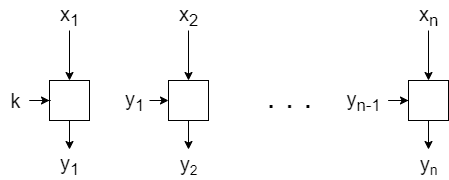
\includegraphics[width=.7\linewidth]{images/Lec14/encCKC.png}
			\caption{Encryption.}
			\label{fig:encCKC}
		\end{subfigure}%
		\begin{subfigure}{.5\textwidth}
			\centering
			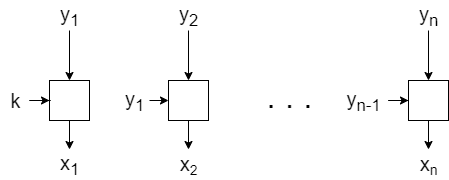
\includegraphics[width=.7\linewidth]{images/Lec14/decCKC.png}
			\caption{Decryption.}
			\label{fig:decCKC}
		\end{subfigure}
		\caption{Encryption and decryption schema of CKC.}
		\label{fig:encdecCKC}
	\end{figure}
	This cipher is insecure because with y$_i$ an attacker can decrypt y$_i+1$ and all the following blocks.
\end{exercise}

\begin{exercise}
	It is proposed an electronic voting scheme where the votes of the electors are sent to a server with a simple encryption E$_k$(v), where v is the id of a candidate. Assume an attacker can intercept messages to the server, show a simple attack scenario (similar to the codebook attack) where the secrecy of the votes is violated without finding k or cryptoanalyzing the cipher. Propose a technique that improves the security of the protocol.
	
	The number of possible candidates is limited. An attacker can send his/her vote x, see E$_k$(x) and find how many people have voted in the same way (violates the privacy). If the possible candidates are two he can know the final result in advance.
	
	To improve the security of the protocol, we can use a stream cipher with random IV, add random bytes to the name of the candidate, etc..
\end{exercise}

\chapter*{Lecture 16}
\textit{Lecture 15 is not present, as it was an exercises class in preparation for the midterm.}

\vspace{10mm}
Proven the Euler Theorem (\ref{teo:eul}), we now want to prove that, using RSA, if we decrypt and encrypted message, we go back to the initial message.

We have that D$_{SK}$(E$_{PK}$(x)) = (x$^b$ mod n)$^a$ mod n = (x$^b$)$^a$ mod n = x$^{ab}$ mod n. We want to prove that x$^{ab}$ mod n = x, that implies D$_{SK}$(E$_{PK}$(x)) = x. To prove this, we will use the Euler Theorem. Note that ab mod $\phi$(n)=1 implies ab=k$\phi$(n)+1 for some k.

\begin{proof}[Correctness of RSA]
	First of all we can notice that 
	\[x^{ab} \ \text{mod} \ n = x^{k\phi(n)+1} \ \text{mod} \ n = (x^{\phi(n)})^kx \ \text{mod} \ n.\]
	
	As we have to prove that $(x^{\phi(n)})^kx \ \text{mod} \ n = x$ and $x$ is different from 0, we can simplify it to $(x^{\phi(n)})^k \ \text{mod} \ n = 1$.
	We split the proof in two cases:
	\begin{itemize}
		\item \textbf{gcd(x,n)=1.} In this case we know that the Euler theorem holds, and we directly have that x$^{\phi(n)}$ mod n = 1, which implies (x$^{\phi(n)}$)$^k$ mod n = 1, giving the thesis;
		\item \textbf{gcd(x,n)>1.} Since x<n, and we know that n=pq, we have that either gcd(x,n)=p or gcd(x,n)=q. We assume gcd(x,n)=p (the proof for the other case is identical).
		
		We can write x=pj for some j. We have that gcd(x,q)=1 (as x<n) that, for Euler Theorem, gives x$^{\phi(q)}$ mod q = 1. 
		
		This implies x$^{\phi(q)\phi(p)}$ mod q = x$^{\phi(n)}$ mod q = 1 (since p and q are primes, x$^{\phi(n)}$ = x$^{\phi(q)\phi(p)}$, moreover 1$^{\phi(p)}$ mod q = 1).
		
		This implies (x$^{\phi(n)}$)$^k$ mod q = 1, giving (x$^{\phi(n)}$)$^k$ = wq + 1 for some w, by definition of modulus.
		
		At this point we obtain:
		\begin{align*}
		(x^{\phi(n)})^k \ x \ \text{mod} \ n &= (wq + 1)x \ \text{mod} \ n\\
		&= (wq + 1)jp \ \text{mod} \ n\\
		&= (wqjp +jp) \ \text{mod} \ n\\
		&= (wqjp + x) \ \text{mod} \ n\\
		&= (njw + x) \ \text{mod} \ n\\
		&= x. 
		\end{align*}
	\end{itemize}
	
	Thus D$_{SK}$(E$_{PK}$(x)) = x and the RSA cipher is correct.
\end{proof}

\begin{example}
	Let's see an example with p=3, q=11, x=2. PK = (b,n) = (3,33); SK = (a,n) = (7,33).\\
	$\phi$(n)=(p-1)(q-1)=2*10=20\\
	x$^{ab}$ mod n = x$^7*3$ mod 33 = x$^{21}$ mod 33 = 2$^{21}$ mod 33 = 2097152 mod 33 = 2.
\end{example}

\subsection*{Inverse modulo}
We have seen that sometimes we need to compute the inverse of a number, for example in RSA we need to compute \textit{a} and \textit{b}, that are one the inverse of the other in module $\phi$(n). Usually we choose \textit{b} and then we compute its inverse to recover \textit{a}. When gcd(b,$\phi$(n))=1, the inverse is guaranteed to exist by the Euler Theorem. In this particular case there is also an efficient algorithm to compute the inverse based on the Euclidean algorithm for computing gcd. 

\subsubsection{Euclidean algorithm}
The idea is to compute the gcd(c,d) (when d$\ne$0) as gcd(d, c mod d), since it can be easily seen that they are the same.

\begin{python}
def Euclid(c,d):
	while d != 0:
		tmp = c % d
		c = d
		d = tmp
	return c
\end{python}

\begin{example}
	Let's try to compute gcd(15,5):
	\begin{itemize}
		\item \texttt{Euclid(15,5)}
		\item d=5$\ne$0
		\item tmp=c\%d=15\%5=0
		\item c=d=5
		\item d=tmp=0
		\item return 5
	\end{itemize}
	Thus gcd(15,5)=5.
\end{example}

This algorithm has a very good complexity, it takes O(k$^3$) steps to terminate, where k is the number of bits, given that the number of iterations is O(k) and that divisions, etc. cost O(K$^2$) steps. O(k) iterations can be proved by observing that every 2 steps we at least halve the value d.

Assume that after one step this is not true, so c mod d > d/2. In the next step, we will compute d mod (c mod d) = d-(c mod d) < d/2 (i.e., d-r(c mod d), with (c mod d) > d/2 $\rightarrow$ r=1) giving the thesis.

We know that halving leads to a logarithmic complexity, i.e., linear with respect to the number k of bis.

\subsubsection{Extended Euclidean algorithm}
We now extend the algorithm so to compute the inverse modulo d whenever gcd(c,d)=1. We substitute the computation of c mod d with:
\begin{center}
	\texttt{q=c/d \#integer division}\\
	\texttt{c-qd  \#this is c\%d}
\end{center}
\begin{example}
	12 mod 5 = 2, q=12/5=2, tmp=12-2*5=2.
\end{example}

We add two extra variables \texttt{e} and \texttt{f} to the algorithm and we save the initial value of d in \texttt{d0} as follows:
\begin{python}
def EuclidExt(c,d):
	d0 = d
	e = 1
	f = 0
	while d != 0:
		q = c/d					#integer division
		tmp = c - q*d		#this is c%d
		c = d
		d = tmp
		tmp = e - q*f		#new computation for the inverse
		e = f
		f = tmp
	if c == 1:
		return e % d0		#if gcd is 1 we have that e is the inverse
\end{python}

\texttt{EuclidExt(c,d)} means that we want to compute the inverse of \texttt{c} modulo \texttt{d}.

\begin{example}
	Let's compute \texttt{EuclidExt(5,17)}:
	\begin{itemize}
		\item q=0, tmp=5, c=17, d=5, tmp=1, e=0, f=1;
		\item q=3, tmp=2, c=5, d=2, tmp=-3, e=1, f=-3;
		\item q=2, tmp=1, c=2, d=1, tmp=7, e=-3, f=7;
		\item q=2, tmp=0, c=1, d=0, tmp=-17 e=7, f=-17.
	\end{itemize}
	e\%d0=7, so e=7 is the inverse, we can see that 7*5 mod 17 = 1.
\end{example}

\begin{exercise}
	Try to compute \texttt{EuclidExt(14,17)}.
	
	\begin{itemize}
		\item q=0, tmp=14, c=17, d=14, tmp=1, e=0, f=1;
		\item q=1, tmp=3, c=14, d=3, tmp=-1, e=1, f=-1;
		\item q=4, tmp=2, c=3, d=2, tmp=5, e=-1, f=5;
		\item q=1, tmp=1, c=2, d=1, tmp=-6, e=5, f=-6;
		\item q=2, tmp=0, c=1, d=0, tmp=17, e=-6, f=17;
	\end{itemize}
	e\%d0=11, so 11 is the inverse, 11*14 mod 17 = 1.
\end{exercise}

In practice, usually the public exponent \textit{b} is fixed and takes the values of the prime number 2$^{16}$+1=65537. If we use at least 3072 bits, it is secure enough.

If an attacker knows $\phi$(n) and n, he can crack everything by solving the system of equation:
\begin{align*}
	\begin{cases}
		n = pq\\
		\phi(n) = (p-1)(q-1)
	\end{cases}
\end{align*}

\begin{exercise}
	Decrypt the following ciphertext, which was encrypted using a Shift Cipher:
	\begin{center}
		\texttt{BEEAKFYDJXUQYHYJIQRYHTYJIQFBQDUJIIKFUHCQD}
	\end{center}
	Using k=16
	\begin{center}
		\texttt{LOOK UP IN THE AIR IT S A BIRD IT S A PLANETS SUPERMAN}
	\end{center}
\end{exercise}

\begin{exercise}
	Compute \texttt{EuclidExt(17,5)}
	
	\begin{itemize}
		\item q=3, tmp=2, c=5, d=2, tmp=1, e=0, f=1;
		\item q=2, tmp=1, c=2, d=1, tmp=-2, e=1, f=-2;
		\item q=2, tmp=0, c=1, d=0, tmp=5, e=-2, f=5;
	\end{itemize}
	e\%d0=3, so 3 is the inverse, 3*17 mod 5 = 1.
\end{exercise}

\begin{exercise}
	We intercept a 'strange' ciphertext 0x000..000115E314E61F9 (i.e., lots of 0s at the beginning) that we know it has been encrypted with RSA under a key of 2048 bits long modulus. What can we immediately conclude about the cipher public key, with very high probability, and how can we trivially compute the plaintext?
	
	The fact that we have a lot of zeros makes us think that the original plaintext was much smaller than the modulus. In other words n is very big and x is so small that encrypting it we do not use the modulus as it is already <n. As we do not used the modulus, we can just do the b-th root of the ciphertext to obtain the original plaintext.
\end{exercise}

\chapter*{Lecture 17}
In RSA we need to generate the two big primes \textbf{p} and \textit{q}. How can we?

The easiest (but not so efficient) solution is to use what is called the "\textbf{Sieve of Eratosthenes}". This algorithm allows us to find all the prime numbers less or equal than \textit{N} and works as follows: we pick all numbers from 2 to \textit{N}, starting from the smallest (2, initially) that we call \textit{p}, we remove from the list all of its multiples 2\textit{p}, 3\textit{p}, ... We iterate the procedure by picking the smallest \textit{p} survived from the previous steps.

\begin{example}
	Let's consider N=10, we will have the list \{2,3,4,5,6,7,8,9,10\}.\\
	Starting from 2 we remove 4,6,8,10, obtaining \{2,3,5,7,9\}.\\
	Consider 3 and remove 9, obtaining \{2,3,5,7\}.\\
	Consider 5 and remove nothing.\\
	Consider 7 and remove nothing.
	
	Thus te the prime numbers remaining in the list are \{2,3,5,7\}.
\end{example} 

It is not needed to check every time all the multiplies, for example, if I am considering p=3, I can skip 6 as because it is a multiple of 2, it has already been deleted when I was considering p=2. For this reason I can skip all the multiplies up to \textit{p}(\textit{p}-1), so I can start checking from \textit{p}$^2$. Obviously if \textit{p}$^2$ is out of my sequence I can stop the list scanning, so the last item \textit{N} of the list will be checked from $\sqrt{N}$, that means that I stop scanning after the \textit{p}=$\sqrt{N}$ element of the list. 

A simple python implementation is the following:
\begin{python}
import sys, math

def Sieve(N):
	Ns = int(math.sqrt(N))						#square root of N
	sieve = set(range(2,N+1))					#sets are good to model the sieve
	for p in range(2,Ns+1):
		if p in sieve: 									#for all survived numbers
			for q in range(p*p,N+1,p): 		#we remove multiples bigger than p
				sieve.discard(q)
	print sieve												#sieve has only primes
\end{python}

\begin{example}
	Sieve(15)=?\\
	Ns=Int(Sqrt(15))=3, we take the lower part of the square root.\\
	sieve=\{2,3,4,5,6,7,8,9,10,11,12,13,14,15\}\\
	p=\{2,3\}\\
	p=2 in sieve, q=\{2$^2$=4,..,15\}\\
	sieve=\{2,3,5,7,9,11,13,15\}\\
	p=3 in sieve, q=\{3$^2$=9,..,15\}\\
	Sieve(15)=\{2,3,5,7,11,13\}
\end{example}

\begin{exercise}
	Sieve(22)=?\\
	Ns=Int(Sqrt(22))=4, we take the lower part of the square root.\\
	sieve=\{2,3,4,5,6,7,8,9,10,11,12,13,14,15,16,17,18,19,20,21,22\}\\
	p=\{2,3,4\}
	p=2 in sieve, q=\{2$^2$=4,..,22\}\\
	sieve=\{2,3,5,7,9,11,13,15,17,19,21\}
	p=3 in sieve, q=\{3$^2$=9,..,22\}\\
	sieve=\{2,3,5,7,11,13,17,19\}\\
	p=4 not in sieve\\
	Sieve(22)=\{2,3,5,7,11,13,17,19\}
\end{exercise}

There is a bed news, unfortunately this algorithm takes at least N steps, meaning that it takes 2$^{3072}$ steps for the smallest RSA modulus, that is too much. We can use another approach, we generate two random numbers and then we check if they are primes or not.

There are many \textit{probabilistic} efficient algorithms for primality test. In 2002, Agrawal, Kayal and Saxena proposed the first \textit{deterministic} algorithm for primality test in the paper "\textbf{PRIMALIY is in P}" published on Annals of Mathematics. This is a very important result, but the proposed algorithm is much slower with respect to existing probabilistic ones, as it costs O(k$^6$) which makes it rather slow for k>3072.

\subsubsection{Miller-Rabin test}
We illustrate one of the most famous probabilistic primality test, due to Miller and Rabin. The algorithm is a \textbf{NO-biased Montecarlo}, i.e., it is always correct for the \textit{NO} answer (meaning that the number is not prime) but can be wrong for the \textit{YES} case (the number is prime). The probability of being wrong, however, is $\le$ than a constant $\epsilon$=$\frac{1}{4}$.

We can repeat the test until the error is small enough. If we run the test \textit{r} times, the probability that it says \textit{YES} and that the number is not prime is less then $\epsilon^r=(\frac{1}{4})^r$. This means that it decreases exponentially with respect to the number of iterations. For example if we pick \textit{r}=128, we have an error with probability less than 1/4$^{128}$, which is less than brute-forcing a typical symmetric key, and so small to be negligible.

The pseudocode of the algorithm is in the following chunk.
\begin{python}
Prime(n):
	write n-1=2^k*m
	pick a random a such that 1<a<n
	b=a^m mod n
	if b==1:
		return True
	for i in range(0,k):
		if b==n-1;
			return True
		b=b*b mod n
	return False
\end{python}

We can always write n-1 as 2$^k$*m as we will not check the primality for even numbers, but only for odd ones. So if I check the primality of an odd number \textit{n}, I can write the even number \textit{n-1} as 2$^k$*m.

\begin{example}
	We want to compute \texttt{Prime(7)}:\\
	n-1=6, it is even and we decompose it as 2$^1$*3. So we have k=1 and m=3.\\
	We compute b as a$^m$ mod n, we choose a=2 (1<a<n), so b=2$^3$ mod 7=1.\\
	b=1 so the algorithm returns \texttt{True}.
	
	In case we choose a=3, we have b=3$^3$ mod 7=6 and also in this time the algorithm returns \texttt{True}, entering the loop.
\end{example}

\begin{exercise}
	Try to compute \texttt{Prime(15)}:\\
	n-1=14, we can decompose it as 2$^1$*7, having k=1 and m=7.\\
	We choose a=2 and we compute b=2$^7$ mod 15=8.\\
	We enter the loop (i=0), b is not equal to n-1 so we compute the new b as b=8*8 mod 15=4.\\
	(i=1) is already too big to stay in the loop so we exit and return \texttt{False}.
\end{exercise}

\begin{exercise}
	Try to compute \texttt{Prime(9)}:\\
	n-1=8, we can decompose it as 2$^3$*1, so k=3 and m=1.\\
	We choose a=2 and we compute b=2$^1$ mod 9=2.\\
	We enter the loop (i=0), b is not equal to n-1 so we compute the new b as b=2*2 mod 9=4.\\
	(i=1) b is different from n-1, the new b is b=4*4 mod 9=7.\\
	(i=2) b is different from n-1, the new b is b=7*7 mod 9=4.\\
	(i=3) is too big to stay in the loop so we exit and return \texttt{False}.
\end{exercise}

\begin{theorem}
	The above algorithm is always correct on False answers (NO-biased).
\end{theorem}

\begin{proof}
	Let's assume, by contradiction, that the algorithm returns False, but the number n is prime. False is only returned at the last step, which means that the algorithm "survived" all the if branches. In particular we have that a$^m$ mod n $\ne$1. Moreover a$^{m2^i}$ mod n $\ne$n-1, for i=0,...,k-1 (for k cycles b=b*b mod n and b $\ne$n-1).
	
	By the assumption that n is prime and by the Euler theorem (a and n are coprime since a<n and n is prime) we know that a$^{\phi(n)}$ mod n = a$^{n-1}$ mod n = a$^{m2^k}$ mod n=1. This is true because, as n is prime, $\phi$(n)=n-1 and we know from the algorithm that we can write n-1=2$^k$*m.
	
	In summary we have:
	\begin{align*}
		a^m mod \ n &\ne 1,n-1\\
		a^{{2^1}m} mod \ n &\ne n-1\\
		a^{{2^2}m} mod \ n &\ne n-1\\
		&...\\
		a^{{2^{k-1}}m} mod \ n &\ne n-1\\
		a^{{2^k}m} mod \ n &= n-1\\		
	\end{align*}
	The last condition is given by the Euler theorem.
	
	It is easy to show that, if n is prime, then the only square roots of 1 modulo n are n-1 and 1.
	
	In fact, r is a square root of 1 iff r$^2$ mod n=1, i.e., r$^2$=z*n+1 for some z, meaning that r$^2$-1=(r+1)(r-1)=z*n which implies (r+1)(r-1)/n=z. Since n is prime, we have that n must divide either (r-1) or (r+1) and so r=-1,1 mod n.
	
	Notice that, if n is not prime there might be square roots of 1 different form 1 and (n-1). For example, for n=8, we have that 5$^2$ mod 8=1, meaning that 5 is a square root of 1 modulo 8.
	
	It is now sufficient to notice that each of the above values is the square root of the preceding one. Since the last one (a$^{m2^k}$) is equal to 1, we have that the previous (a$^{m2^{(k-1)}}$) is a square root of 1 modulo n, i.e., it is 1 or n-1.
	
	Now we know that it is different from n-1 which implies that it is 1. We iterate backward this on all the values until we got a$^m$ mod n=1 which gives a contradiction.
	
	This proves that the algorithm can never return \texttt{False} if n is prime.

\end{proof}

A working python implementation is the following:
\begin{python}
def Prime(n):
	m = n-1
	k = 0
	while (m&1 == 0): 		#while m is even
		m = m>>1
		k += 1
	a = random.randrange(2,n)
	b = squareAndMultiply(a.m,n)
	if b == 1:
		return True
	for i in range (k):
		if b == n-1:
			return True
		b = b*b % n
	return False
\end{python}

So, how can we generate big primes? We simply generate them at random and we test their primality. This takes about ln(n) steps, where n is the upper bound of the interval we choose from. It can be proved, in fact, that about 1 out of ln(n) numbers less than n are prime. For example, if we want 512 bits of size (for a modulus 1024), we have that ln(n) = log$_2$(n)*ln(2) $\approx$ 512*0.7 $\approx$ 358. Thus, on average, after 358(716) attempts we should find a prime number of size 512 (1024) bits. 

Notice that, the Miller-Rabin algorithm should be iterated to lower as needed the probability of error in case of successful answer. In the original paper, the probability is bounded by 1/4, in a subsequent paper it has been shown that the algorithm is much more precise than that. In practise the suggested number of iterations from NIST are 7,4 and 3 for 512, 1024 and 1536 bits, with an error probability of 2$^{-100}$ , meaning that the test requires very few iterations to give a prime with high probability.

\subsubsection{Case study: OpenSSL}
\begin{wrapfigure}[11]{r}{0.4\textwidth}
	%\centering
	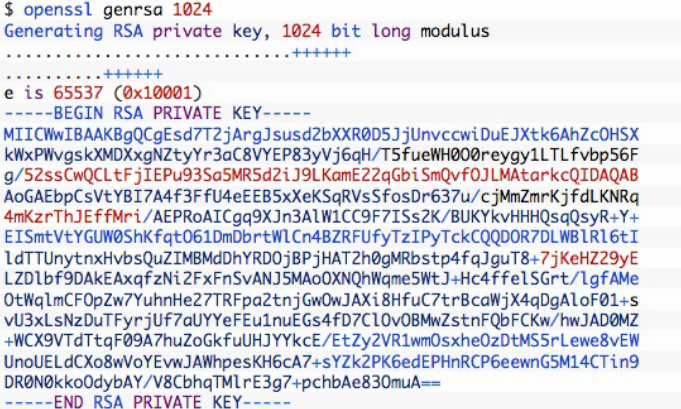
\includegraphics[width=0.37\textwidth]{images/lec17/openssl.png}
	\caption{Generation of a Private Key using OpenSSL.}
	\label{fig:openssl}
\end{wrapfigure}

\textbf{OpenSSL} is a software library for applications that need to secure communications over the internet widely used against eavesdropping and to be sure of the identity of the party at the other end. It contains an open source implementation of the SSL and TLS protocols. It supports a lot of different cryptographic algorithms: \textit{ciphers} (such as AES, Blowfish, DES, IDEA, ..), \textit{cryptographic has functions} (MD5, SHA-1, ...) and \textit{public-key cryptography} (RSA, DSA, ...).

In Figure \ref{fig:openssl} we can see the generation of a Private Key using OpenSSL. It uses a number of iterations slightly bigger than the one suggested above. For a 1024 key as in figure we have 6 occurrences of '+', which represent 6 iterations of the Miller-Rabin test.

\chapter*{Lecture 18}
As already said, security of RSA is based on the secrecy of $\phi$(n)=(p-1)(q-1). We know that if n is big enough, its factorization is a hard problem so that the attacker cannot go back to p and q. It is however trivial to see that computing $\phi$(n) is at least as difficult as factoring n. Given an algorithm that computes $\phi$(n), to compute p and q it is enough to solve the system of equations:
\begin{align*}
\begin{cases}
	n = pq\\
	\phi(n) = (p-1)(q-1)
\end{cases}
\end{align*}

We can make another observation: it could be possible, in principle, to compute the private exponent without necessarily computing $\phi$(n). It can be proved that this would allow to factorize n.

\begin{theorem}
	Given an algorithm that computes the exponent \textit{a}, we can write a probabilistic "Las Vegas" algorithm that factorizes \textit{n} with probability at least 1/2.
\end{theorem} 

As for Monte Carlo algorithms, we can iterate a Las Vegas algorithm as needed. This proves that if an exponent is leaked, then \textit{n} is compromised, thus breaking a private key is as difficult as factorizing. Notice also that, once we leak a private key, the modulus is no more secure. This implies that n should never be reused for different key pairs: any time we generate a key pair, we need to generate a new modulus n.

We have already observed that implementations of RSA use small encryption exponents (typically 2$^{16}$+1=65537) to improve the performance of encryption function. We will now discuss some attacks that are possible if we choose an excessively small exponent such as 3.

\subsection*{Attack 1: same message encrypted under different modules}
Suppose the same message m is sent encrypted under at least three different public keys (3,$n_1$), (3,n$_2$), (3,n$_3$) giving the three ciphertexts c$_1$, c$_2$, c$_3$, such that c$_i$ = m$^3$ mod n$_i$. Notice that, modules n$_1$, n$_2$, n$_3$ are very likely to be coprime as they will not share their prime factors.

\begin{theorem}
	Chinese Remainder Theorem: Let n$_1$, ..., n$_k$ be integers >1, and N=n$_1$*n$_2$*...*n$_k$. If the n$_i$ are pairwise coprime, and if a$_1$, ..., a$_k$ are integers such that 0$\le$a$_i\le$n$_i$ for every i, then there is one and only one integer x such that 0$\le$x$\le$N and x mod n$_i$=a$_i$ for every i. 
\end{theorem}
 
The Chinese Remainder Theorem applies and proves that there exists a unique x<n$_1$*n$_2$*n$_3$, such that x mod n$_i$=c$_i$, with an efficient way to compute it. In our case x will be m$^3$.

Notice that m<n$_i$, which implies m$^3$<n$_1$*n$_2$*n$_3$. By definition of c$_i$ we also have c$_i$=m$^3$ mod n$_i$. Thus, the unique x given by the Chinese Reminder Theorem must be equal to m$^3$. It is now enough to compute (x)$^{1/3}$ to get m.

\begin{example}
	Let's consider m=2, n$_1$=3, n$_2$=5, n$_3$=7.\\
	c$_1$ = m$^3$ mod n$_1$ = 8 mod 3 = 2\\
	c$_2$ = m$^3$ mod n$_2$ = 8 mod 5 = 3\\
	c$_3$ = m$^3$ mod n$_3$ = 8 mod 7 = 1\\
	
	The attacker sees the three ciphertexts 2,3,1.
	
	The Chinese Reminder Theorem tells us that $\exists$x: x<3*5*7\\
	Moreover it is true that 0$\le$c$_i$<n$_i$ for all i. Thus it is true that there exists a unique x such that x mod n$_i$=c$_i$.
	
	We will get that x=8, thus x=m$^3$=8, so m=$\sqrt[3]{8}$=2 that is our message.
\end{example} 

We can say that, in general, \textit{b} encryptions of the same message m, under different keys are enough to recover m. Picking \textit{b}=65537 makes this attack quite unlikely.

Moreover the attack can be prevented by a randomized padding scheme such as \textbf{PKCS1} which transforms message m into a k-bits long message
\begin{center}
	\texttt{EM=0x00||0x02||PS||0x00||m},
\end{center}
where PS is a sequence of random bytes different from 0. In this way any time we encrypt m, in fact we encrypt a different plaintext. Notice that PKCS1 enables padding-oracle attacks and is superseded by the more secure Optimal Asymmetric Encryption Padding (OAEP).

\subsection*{Attack 2: small messages}
Padding is also needed because of the following trivial attack on \textit{small messages} encrypted under small exponents (1 message here is enough). Consider a small message m encrypted with exponent 3. we have then y=m$^3$ mod n and it might be the case that m$^3$<n meaning that y=m$^3$ mod n=m$^3$. To decrypt it is enough to compute y$^{1/3}$. Padding prevents this attack by making the size of m$^3$ close to the size of the modulus n.

\subsection*{Partial information}
It could be possible that an attacker is able to partially recover the plaintext. This attack has stronger assumptions but so it is a bit harder to run. Let y=E$_{PK}$(x).

Examples of partial information are:
\begin{itemize}
	\item parity(y): returns the parity of the plaintext;
	\item half(y): tells if the plaintext is less than half of the modulus n.
\end{itemize}

We can define them as:
\[
parity(y)=
\begin{cases}
	0 & \text{if}\  x \ \text{is even}\\
	1 & \text{otherwise}
\end{cases}
\]
\[
half(y)=
\begin{cases}
0 & \text{if} \ 0\le x\le n/2\\
1 & \text{otherwise}
\end{cases}
\]

We claim that if an attacker knows these information, he is able to decrypt the ciphertext. First, we show that the latter can be defined based on the former. This means that an attacker needs only one of the two information to decrypt the message.

The result exploits the following fundamental property of RSA.

\begin{theorem}
	RSA multiplicative property: RSA cipher is such that E$_{PK}$(x$_1$)E$_{PK}$(x$_2$) mod n=E$_{PK}$(x$_1$x$_2$ mod n).
\end{theorem}

\begin{proof}
	It is enough to apply the definition of encryption:
	\begin{align*}
		E_{PK}(x_1)E_{PK}(x_2) \text{ mod n} &= x_1^bx_2^b \text{ mod n}\\
		&= (x_1x_2)^b \text{ mod n}\\
		&= (x_1x_2 \text{ mod n})^b \text{ mod n}\\
		&= E_PK(x_1x_2 \text{ mod n})
	\end{align*}
\end{proof}

We can now prove that
\begin{center}
	half(y)=parity(E$_{PK}$(2)y mod n).
\end{center}
\begin{proof}
Notice that, parity(E$_{PK}$(2)y mod n)=parity(E$_{PK}$(2)E$_{PK}$(x) mod n)=parity(E$_{PK}$(2x mod n)) for the previous property.

If half(y)=0, by definition we have 0$\le$x<n/2 which implies 0$\le$2x<n, thus 2x mod n=2x which is certainly even, i.e., parity(E$_{PK}$(2)y mod n)=parity(E$_{PK}$(2x mod n))=0 (by definition of parity).

If half(y)=1, then n/2$\le$x<n, which implies n$\le$2x<2n, thus 2x mod n=2x-n which is certainly odd since 2x is even and n is odd (it cannot be a multiple of 2). As a consequence parity(E$_{PK}$(2)t mod n)=parity(E$_{PK}$(2x mod n))=1.

\end{proof}

At this point, the following holds:
\begin{theorem}
	Given al algorithm that computes half(y) or parity(y), it is possible to compute the whole plaintext x.
\end{theorem}

\begin{proof}
	Since half(y) can be defined in terms of parity(y), it is sufficient to prove that having half(y) we can compute x.
	
	It is enough to do a binary search, each time multiplying by E$_{PK}$(2) the ciphertext, and getting the left/right interval, depending on the value of half.
	
	It is obvious that this works for the first step (definition of half exactly tells us whether x belongs to the first half or the second half of the interval).
	
	Then think of half(yE$_{PK}$(x)). It is 0 when 2x mod n<n/2 which happens when 0$\le$x<n/4 or n/2$\le$x<3n/4, since we respectively obtain 0$\le$2x<n/2 and n$\le$2x<3n/2, the latter implying n mod n$\le$2x mod n<3n/2 mod n, i.e., 0$\le$2x mod n<n/2.
	
	This reasoning can be applied, similarly, to next steps until a single solution survives. Since each time the interval is split in two, the number of steps is $\lceil$log$_2$(n)$\rceil$. 
\end{proof}

\chapter*{Lecture 19}
We will now see a \textit{chosen ciphertext attack} to RSA, it is a simple attack in which the attacker can ch	oose ciphertexts to decrypt. The challenge is to decrypt a ciphertext y' by asking for decryptions of different ciphertexts y$_1$,...,y$_n$. The attack proceeds as follows: she picks a random r such that 1<r<n and is invertible modulo n.

The inverse can be computed using the extended Euclidean Algorithm (if it fails, we pick another random r). The attacker asks for decryption of y$_1$=y'E$_{PK}$(r) mod n. She obtains the plaintext x$_1$=x'r mod n, where x' is the decryption of y'. It is now sufficient to multiply this number by r$^{-1}$ mod n to get x'.

\begin{exercise}
	Try with n=pq=3*7=21, public key (17,21).
	
	First of all we need to compute the secret key, we need to find a such that a*b mod $\phi$(n)=1, so a*17 mod 12=1, we have a=5, so the secret key is (5,21).
	
	Now we need to choose r: 1<r(=11)<21. We have to check if it is invertible: r*r$^{-1}$ mod 21=1, 11*r$^{-1}$ mod 21=1, r$^{-1}$=2 is the inverse.
	
	The encryption of our r is E$_{PK}$(r)=E$_{PK}$(11)=11$^{17}$ mod 21=2.\\
	Let us assume we want to find x'=2, thus y'=2$^{17}$ mod 21=11.\\
	So y$_1$=y'E$_{PK}$(r) mod n=11*2 mod 21=1. Thus x$_1$=1$^5$ mod 21=1.\\
	The attacker gets x'=x$_1$r$^{-1}$ mod 21=1*2 mod 21=2.
\end{exercise}

\section*{Digital signatures}
Asymmetric key cryptography is also employed to develop \textit{digital signature schemas} (i.e., a digital counterpart of classic signature on paper). There are some important features of classic signature that deserve to be discussed in order to understand which are the basic expected properties of any good signature scheme.

Classic signature is physically part of the signed document. We should avoid that a signature can be cut-and-pasted to a different document. So, the signature will depend on the signed document: two different documents signed by the same entity will have different signatures.

Classic signature is verified by comparing it to an official reference signature. This is not possible in the digital world since signature of different documents should always be different. We need a mechanism to verify a signed document with respect to an entity (the signer).

Document signed on paper cannot be easily copied. In the digital world we can trivially cut-and-paste bytes so any signed document can be replicated many times. In certain applications (e.g., e-commerce) signature needs to be integrated with mechanisms to avoid uncontrolled replicas.

Imagining that Bob wants to send a message to Alice, signed using the digital signature, we want that:
\begin{itemize}
	\item to sign you need to know the private key;
	\item to verify you need the public key.
\end{itemize}
We remember that only Bob knows his private key and everyone knows Bob's public key.

\begin{definition}
	A digital signature scheme consists of two functions:
	\begin{itemize}
		\item Sig$_{SK}$(x) generates the signature of x using a private key SK;
		\item Ver$_{PK}$(x,y) checks the validity of signature y on message x using a public key. It returns true if the signature is valid and false otherwise.
	\end{itemize}
\end{definition}

We now discuss how the RSA cipher can be used to implement a digital signature scheme. We let:
\begin{align*}
	Sig_{SK}(x) &= D_{SK}(x)\\
	Ver_{PK}(x,y) &= 
	\begin{cases}
	true & \text{if}\  E_{PK}(y)=x\\
	false & \text{otherwise}
	\end{cases}
\end{align*}
Note that, encryption and decryption of RSA are the same function:
\begin{itemize}
	\item Sig$_{SK}$(x)=D$_{SK}$(x)=x$^a$ mod n;
	\item Ver$_{PK}$(x,y)=true if E$_{PK}$(y)=y$^b$ mod n=x.
\end{itemize}

Note that it is impossible to copy the signature without knowing SK and it is possible to check the signature knowing PK.

\begin{example}
	Consider p=7, q=13, PK=(5,91), SK=(29,91) and x=35.
	
	Sig$_{SK}$(35)=35$^{29}$ mod 91= 42.
	
	We check the signature by computing Ver$_{PK}$(35,42)=42$^{5}$ mod 91=35.
	
	Thus the signature is valid.
\end{example}

This scheme is not yet satisfactory as it does not satisfy the security property that without knowing the private key it is computationally infeasible to find a message x and a signature y such that Ver$_{PK}$(x,y) holds, i.e., y is a valid signature for x. We show different ways to find x and y such that Ver$_{PK}$(x,y) holds.

\subsection*{Problems and attacks}
\subsubsection{Forging a "random" message}
We (in the middle) pick an arbitrary signature y, we compute the corresponding signed message as E$_{PK}$(y) and we forward this to the receiver instead of x. Since Ver$_{PK}$(E$_{PK}$(y),y)=true, by definition, the receiver does not notice anything wrong, but what he should have received is x and not E$_{PK}$(y) (so he is just checking something wrong).

\subsubsection{Multiplying signed messages}
If we have two signed message x$_1$, x$_2$ with signatures y$_1$, y$_2$, then y$_1$*y$_2$ mod n is the signature of a message x$_1$*x$_2$ mod n. If the expected message is just a number with no particular format or padding, this attack might be very effective.

In addition to the discussed forging attacks, the above defined signature has different drawbacks, for example, the size of the signature is at least the same as the size of the message, meaning that we have to send at least double the size of signed data.

The properties we would like to have are:
\begin{itemize}
	\item \textbf{authenticity}: the origin of the message is correctly identified;
	\item \textbf{non-repudiation}: the sender cannot deny the transmission of a message;
	\item \textbf{integrity}: the information can be modified only by the authorized entities.
\end{itemize}

Can we assure integrity? If a message is bigger than the RSA modulus, we would need to split it into blocks, in this way the attacker may remove blocks.

The solution to all these issues, including the problem of forging, is the adoption of \textbf{cryptographic hash functions}.
\begin{definition}
	A hash function h: X$\rightarrow$Z is a function taking an arbitrarily long message x and giving a digest z of fixed length.
\end{definition} 

When used in cryptography, these functions are required to satisfy specific properties that we discuss below through our running-example.

We modify our proposed signature scheme based on RSA so to prevent all of the discussed problems. Let h be a hash function:
\begin{align*}
	Sig^h_{SK}(x) &= D_{SK}(h(x))\\
	Ver^h_{PK}(x,y) &= 
	\begin{cases}
	true & \text{if}\  E_{PK}(y)=h(x)\\
	false & \text{otherwise}
	\end{cases}
\end{align*}

Thus, to sign x we decrypt its hash under the private key, to check the signature, we encrypt the signature under the public key, we recompute the hash on x and we compare the two results.

Since the hash is of fixed length, it is enough to take it smaller than the RSA modulus to solve all the issues related to the size of the signature and the necessity of encryption modes.

Let's consider the simplest attack (in the scheme without hash) where, given an arbitrary signature y, we compute the corresponding signed message as E$_{PK}$(y). In the hash-based scheme, E$_{PK}$(y) would provide the hash of the signed message, so if we are able to find an x such that h(h)=E$_{PK}$(y), we will have that Ver$^h_{PK}$(x,y)=true. this leads to our first property for cryptographic has functions.

\begin{definition}
	A hash function h is preimage resistant (or one-way) if given z it is infeasible to compute x such that h(x)=z. 
\end{definition}  

\begin{example}\label{ex:hashxor}
	Let's consider a simple hash function h(x) that splits the message x into blocks x$_1$, x$_2$, .., x$_n$ of a fixed size k and computes the bit-wise xor of all blocks:
	\begin{align*}
	h(x)=x_1 \oplus x_2 \oplus .. \oplus x_n.
	\end{align*}
	
	This function is clearly not preimage resistant, given a digest z we can easily find preimages:\\
	E.g., z, z||0, z||x||x, z||x||y||x$\oplus$y, .. here 0 denotes the block of k zeros and || the concatenation of blocks, all are correct preimages of z.
\end{example}

Notice that preimage resistance also prevents forging based on RSA multiplicative property. If we have two signed messages x$_1$, x$_2$ with signatures y$_1$ and y$_2$, then y$_1$*y$_2$ mod n is the signature of a message whose hash is the same as z=h(x$_1$)*h(x$_2$) mod n. Finding such message x means that we can compute a preimage x of h such that h(x)=z, but this is ruled out by preimage resistance.

It appears that adopting hash-based RSA signature scheme in which the hash function is preimage resistant solves all the issues. Unfortunately, we also have to consider potential problems deriving from the adoption of hashes. Since a has summarizes messages as fixed-length digests, it can of course occur that different messages have the same hash. For example we might have different x$_1$ and x$_2$ such that h(x$_1$)=h(x$_2$). Then, Sig$^h_{SK}$(x$_1$)=Sig$^h_{SK}$(x$_2$), so the two messages have the same signature.

Consider an attack in which, given a message x$_1$ and its signature y$_1$, the attacker computes a x$_2$ such that h(x$_1$)=h(x$_2$). Then y$_1$ is a valid signature for x$_2$, meaning that the attacker has forged a signature for a message of its choice.

\chapter*{Lecture 20}
We remember that in a chosen-plaintext attack, the adversary can (possibly adaptively) ask for the ciphertexts of arbitrary plaintext messages. The adversary can interact with an encryption oracle, viewed as a black box.

\begin{example}
	During World War II, US Navy cryptoanalysts understood that Japan was planning to attack location "AF". They thought that "AF" could have stand for "Midway Island" as Hawaii Islands started with "A". To prove this, they asked the US forces at Midway to send a plaintext message about low supplies. The Japanese intercepted the message and reported to their superior thath "AF" was low on water, confirming the Navy's hypothesis and allowing them to position their force to win the battle.
\end{example}

\begin{definition}
	A hash function is second-preimage resistant if given x$_1$, it is infeasible to compute x$_2$ such that h(x$_1$)=h(x$_2$).
\end{definition}

If we assume the attacker is allowed to ask for signatures (similarly to what happens in a chosen-plaintext attack), it might still happen that he chooses two different messages x$_1$ and x$_2$ (both of them) with the same hash and asks for a signature on x$_1$. In this way he obtains a valid signature for x$_2$.

\begin{example}
	Suppose the attacker manages to generate two messages that look the same, but one (x$_2$) gives more advantage than the other (x$_1$), such as in two contracts with different prices. The attacker convinces the other party to sign x$_1$ which looks reasonable but obtains a signature on x$_2$ that has an outrageous price in it. For this reason, we need a new property for hash functions.
\end{example}

\begin{definition}
	A hash function is collision resistant if it is infeasible to compute different x$_1$ and x$_2$ such that h(x$_1$)=h(x$_2$). 
\end{definition}

Differently from second-preimage resistance, here the attacker can choose both x$_1$ and x$_2$ and he is not given an x$_1$ that he has to find a second-preimage of. Thus, this latter property implies the previous one, i.e., if a has is collision resistant, it is also second-preimage resistant.

We need our has function to be collision resistant. It is possible to prove that collision resistance also implies preimage resistance. Thus, if a hash function is collision resistant, it has all of the above mentioned properties. This holds under the assumption that the number of messages we can hash is at least twice as the number of digests.

\begin{theorem}
	Let h:X$\rightarrow$Z be a collision resistant hash function such that |X|$\ge$2|Z|. Then h is also preimage resistant.
\end{theorem}
We prove the following equivalent fact: if h is not preimage resistant, then h is not collision resistant.

To do so, we show that given an algorithm Invert(z) for inverting h (that breaks preimage resistance), we can write a Las Vegas probabilistic algorithm that finds a collision. The algorithm is, in fact, rather simple: we pick a random message, we compute its hash and we invert it using the given algorithm Invert(z). If we find a different message we are done, otherwise, if we are unlucky and get the initial message, we fail. the pseudocode of the algorithm is the following:
\begin{python}
FindCollisions:
	choose a random x1 in X
	z=h(x1)
	x2=Invert(z)
	if x1 != x2:
		output(x1,x2)
	else:
		FAIL
\end{python}

If I fail, I run again the algorithm, picking another x1.

Correctness of solution is obvious since x1 and x2 have the same hash, meaning that they have a collision. We now prove that failure happens with probability at most 1/2.

\begin{proof}
	Since we have |Z| possible digests, we have that Invert(z) returns exactly |Z| preimages, one for each digest, and these are the unlucky cases, i.e., the messages that once hashed will be mapped back to themselves. 
	
	Thus, the good cases are exactly |X|-|Z| and the probability of success is
	\[\frac{|X|-|Z|}{|X|}\ge\frac{|X|-1/2|X|}{|X|}=\frac{1/2|X|}{|X|}=\frac{1}{2}.\]
	
	As a consequence, we fail with probability $\le$ 1/2. As any Las Vegas algorithm, this can be iterated as needed. For r iterations we have that the probability of failure is $\le$1/2$^r$.
\end{proof}

In the example \ref{ex:hashxor}, we showed that that hash function is not preimage resistant, since given a digest z, we can easily find preimages. Thus, it is also clearly not collision and second preimage resistant. Given x=x$_1$,x$_2$,..,x$_n$, we have for example that x$_2$,x$_1$,..,x$_n$ has the same digest, we can swap blocks as xor is commutative. Moreover, we can add zero blocks, add whatever block twice, add a block and then add it xored with the original message, and so on.

\begin{example}
	We consider another simple hash function g(x)=E$_{h(x)}$(0), i.e., we use the previous hash (the one with the xor) to obtain a key for a cipher and we encrypt the constant 0 under that key. This hash function is preimage resistant if the adopted cipher is resistant to known-plaintext attacks. In fact, finding h(x) from g(x) corresponds to breaking the cipher (h(x) is the key), knowing the plaintext 0 and the ciphertext g(x). However, it is neither collision resistant nor second preimage resistant, as collision on h (found given the xor) are collisions on g and we have shown above that h is not collision resistant.
\end{example}

\subsection*{The birthday attack}
We have discussed important properties of hash functions that are needed, for example, when developing a hash-based signature scheme. Collision resistance is the strongest of such properties: it is important that hash functions are carefully designed so to make the computation of collisions infeasible. As for cryptography, the attacker can try to break a function by brute force.

For the case of hash function, brute forcing is much simpler than expected, thanks to the so-called \textbf{Birthday Attack}. This funny name comes from an analogy to the famous birthday paradox: \textit{given a group of 23 people, with probability 1/2 there are at least two of them with the same birthday (day and month, not year). With a group of 41, the probability is already around 90\%}. This fact is so counter-intuitive to be called paradox.

The analogy with cryptographic hash functions is immediate: birthday can be seen as a hash function from any person to a fixed-size set of 365 days of the year. Two people having the same birthday represent a collision on the hash function. The fact collisions are so likely means that brute-forcing a hash function might be much easier than expected, and we will give a precise estimate of this.

We assume people being mapped to birthdays in a uniform way. This assumption fits very well with cryptographic hashes as they usually behave that way to make the find of a collision or a preimage as much hard as possible. We will now compute the probability that in a group of k people, none share the birthday.

For the first person, any birthday is fine. Thus, we have probability 1 of success. The second person should not share the birthday with the first one, meaning that we have probability 364/365 of success, and so on. We require that these events all occur together, giving a probability of $\prod_{i=0}^{k-1}\frac{365-i}{365}$. So, the probability of a collision is 1-$\prod_{i=0}^{k-1}\frac{365-i}{365}$. The following python code compute this probability.
\begin{python}
from decimal import *
def Birthday(k):
	r=1
	for in in range(k):
		r = r*(365-1)
	return 1 - (Decimal(r)/Decimal(365**k))
\end{python}

It is now useful to find a relation between the number giving probability 1/2 (in this case 23) and the number of digests, as this will allow us to estimate the cost of a brute force attack. We let n be the number of digests (365 for the birthday paradox). We reason as follows: the probability that we do not find a collision is \[\prod_{i=0}^{k-1}\frac{n-i}{n} = \prod_{i=0}^{k-1}\left(1-\frac{i}{n}\right).\]
Now from analysis we know that, for small x, 1+x$\approx$e$^x$ (note that from Taylor series e$^x$=1+x+$\frac{x^2}{2!}$+$\frac{x^3}{3!}$+...).

If 1+x $\approx$ e$^x$, then 1-1/n=e$^{-1/n}$. Thus, the probability of finding a collision is:
\[\epsilon \approx 1-\prod_{i=0}^{k-1}e^{-\frac{i}{n}} = 1-e^{-\frac{(k-1)k}{2n}}.\]
Thus 1-$\epsilon \approx e^{-\frac{(k-1)k}{2n}}$ and so we get ln(1-$\epsilon$)$\approx -\frac{(k-1)k}{2n}$. Thus 2$n$ ln(1/(1-$\epsilon$)) $\approx k^2-k$ (as log x$^n$ = n log x, here n=1).\\By a further approximation (disregarding k), we get k $\approx\sqrt{2n \ \text{ln}(1/(1-\epsilon))}$.

For $\epsilon$=1/2, this gives k$\approx$1.17$\sqrt{n}$. Thus, a brute-force attack on a hash function with n digests, finds a collision with probability 1/2 after about $\sqrt{n}$ attempts. For example, if a hash function returns digests of 128 bits, it takes about $\sqrt{2^{128}}=2^{64}$ trials to break it. So, to have the same security we have with a 128 bits cipher, we need double the length, i.e., 256 bits of hash.

\subsection*{Commonly used hash functions}
One of the most famous cryptographic hash function is \textbf{MD5} (Message Digest 5), by Ron Rivest (the 'R' of RSA). It is a 128-bits hash used in many applications. Recently, it has been shown to be not collision resistant, moreover the relatively small size allows for a birthday attack in only 2$^{64}$ steps. There exists a \textit{collision attack} that can find collisions within seconds on a computer with a 2.6 GHz Pentium 4 processor (complexity of 2$^{24.1}$). There is also a chosen-prefix attack that can produce a collision for two inputs with specified prefixes within hours, using off-the-shelf computing hardware (complexity 2$^{39}$).

The most common alternative to MD5 is \textbf{SHA} (Secure Hash Algorithm). On 2/23/2017, Google announced the SHAttered attack, in which they generated two different PDF files with the same SHA-1 hash in roughly 2$^{63.1}$ SHA-1 evaluations. It is 100.000 times faster than brute forcing a SHA-1 collision with a \textit{birthday attack}, which is estimated to take 2$^{80}$ SHA-1 evaluations. The attack required "the equivalent processing power as 6.500 years of single-CPU computations and 110 years of single-GPU computations". The second generation SHa (SHA-2) has a variable digest size from 224 to 512 bits. It is not vulnerable to the collision attacks and the length makes birthday attack infeasible. The NIST has selected SHA-3, with a process similar to the one for selection AES. SHA-3 is the one that we should use in practice.
\end{document}


